% Use only LaTeX2e, calling the article.cls class and 12-point type.

\documentclass[12pt]{article}

% Users of the {thebibliography} environment or BibTeX should use the
% scicite.sty package, downloadable from *Science* at
% http://www.sciencemag.org/authors/preparing-manuscripts-using-latex 
% This package should properly format in-text
% reference calls and reference-list numbers.

\usepackage{scicite}

\usepackage{times}

\usepackage{graphicx,float}

%setup for commenting during editing
\usepackage{xcolor}
\newcommand{\tom}[2]{{\color{red}{#1}}\footnote{\textit{\color{red}{#2}}}}
\newcommand{\josh}[2]{{\color{blue}{#1}}\footnote{\textit{\color{blue}{#2}}}}

% for adjusting the sizes of tables
\usepackage{adjustbox}
% for setting up equations
\usepackage{amsmath}

% The preamble here sets up a lot of new/revised commands and
% environments.  It's annoying, but please do *not* try to strip these
% out into a separate .sty file (which could lead to the loss of some
% information when we convert the file to other formats).  Instead, keep
% them in the preamble of your main LaTeX source file.


% The following parameters seem to provide a reasonable page setup.

\topmargin 0.0cm
\oddsidemargin 0.2cm
\textwidth 16cm 
\textheight 21cm
\footskip 1.0cm


%The next command sets up an environment for the abstract to your paper.

\newenvironment{sciabstract}{%
\begin{quote} \bf}
{\end{quote}}



% Include your paper's title here

\title{Microbial symbionts buffer hosts from the consequences of environmental stochasticity} 


% Place the author information here.  Please hand-code the contact
% information and notecalls; do *not* use \footnote commands.  Let the
% author contact information appear immediately below the author names
% as shown.  We would also prefer that you don't change the type-size
% settings shown here.

\author
{Joshua C. Fowler,$^{1\ast}$ Shaun Ziegler,$^{2}$ Kenneth D. Whitney,$^{2}$\\
	 Jennifer A. Rudgers,$^{2}$ Tom E. X. Miller $^{1}$\\
\\
\normalsize{$^{1}$Rice University, Department of BioSciences, Houston, TX, 77005}\\
\normalsize{$^{2}$University of New Mexico, Department of Biology, Albuquerque, NM, 87131}\\
\\
\normalsize{$^\ast$To whom correspondence should be addressed; E-mail:  jcf3@rice.edu.}
}

% Include the date command, but leave its argument blank.

\date{}



%%%%%%%%%%%%%%%%% END OF PREAMBLE %%%%%%%%%%%%%%%%



\begin{document} 

% Double-space the manuscript.

\baselineskip24pt

% Make the title.

\maketitle 


% Place your abstract within the special {sciabstract} environment.

\begin{sciabstract}
	ABSTRACT: 
    The ability to cope with the negative consequences of environmental stochasticity will be critical to species' persistence in increasingly variable future climates. 
	Practically all organisms host microbiota that may promote host resilience in the face of climate stress. 
	Yet, how microbial symbionts modify host responses to environmental stochasticity is poorly understood, because the long-term data necessary to detect such an influence is rarely available. 
	Using stochastic demographic models parameterized from a unique 14-year symbiont-removal experiment with seven grass species and their \emph{Epichlo\"{e}} fungal endophytes, we show, for the first time, that microbial symbiosis elevates host fitness by dampening year-to-year fluctuations in demographic performance. 
	This effect is stronger in host species with ``fast'' life histories that lack the intrinsic buffering provided by longevity. 
	Model simulations revealed that increasing environmental stochasticity, as expected under global change, amplifies the importance of variance buffering as a pathway of host-symbiont mutualism, surpassing the mean fitness benefits that are the focus of most previous studies. 
	The stabilizing influence of microbial symbiosis is an important but cryptic mechanism of host resilience to global change.\tom{}{The abstract is limited to 125 words. This is over the limit.} 

\end{sciabstract}


\subsubsection*{One sentence summary suggestions:}
Microbial symbionts buffer hosts against negative effects of environmental variability.

% In setting up this template for *Science* papers, we've used both
% the \section* command and the \paragraph* command for topical
% divisions.  Which you use will of course depend on the type of paper
% you're writing.  Review Articles tend to have displayed headings, for
% which \section* is more appropriate; Research Articles, when they have
% formal topical divisions at all, tend to signal them with bold text
% that runs into the paragraph, for which \paragraph* is the right
% choice.  Either way, use the asterisk (*) modifier, as shown, to
% suppress numbering.

\section*{Main Text}

Global climate change is driving increases in the variability of precipitation patterns and the frequency of extreme weather events \cite{IPCC2012managing,seneviratne2012changes,stocker2013technical}. 
The consequences of this increased variability have received less attention than effects on mean climate conditions. 
Incorporating variability into forecasts of population dynamics is a key step towards improved predictions of the future.
Classic theory predicts that long-term population growth rates (equivalently, population mean fitness) will decline under increased environmental variability due to negative effects of bad years that outweigh the positive effects of good years (a consequence of nonlinear averaging) \cite{lewontin_population_1969,tuljapurkar_population_1982}.
For example, in unstructured populations, the long-term stochastic growth rate in fluctuating environments ($\lambda_s$) will always be lower than the growth rate averaged across environments ($\overline{\lambda}$) by an amount proportional to the environmental variance ($\sigma^2$): 
\begin{equation}
	 log(\lambda_s)  \approx log(\overline{\lambda}) - \frac{\sigma^2}{2\overline{\lambda}^2}
\end{equation}

\noindent Populations structured by size or stage similarly experience costs of variability \cite{cohen1979comparative,tuljapurkar2013population}.
Thus, there are two pathways to increase population viability in a variable environment: increase the mean growth rate and/or dampen temporal fluctuation in growth rates, also called variance ``buffering''.

Both the characteristics of species and the properties of their environment can buffer demographic fluctuations, including life history traits such as longevity \cite{pfister1998patterns, morris2008longevity}, correlations among vital rates \cite{compagnoni2016effect}, transient shifts in population structure \cite{ellis2013role}, the magnitude of environmental variability \cite{rodriguez2021limits}, or the degree of environmental autocorrelation \cite{tuljapurkar1980population,fieberg2001stochastic}. 
These characteristics determine the risks of population extinction faced by species \cite{menges2000applications} and underlie conservation management strategies promoting ecosystem resilience \cite{kuparinen2016fishing}. 
Yet little is known about how biotic interactions alter demographic variability \cite{hilde_demographic_2020}. 

Most multicellular organisms host symbiotic microbes that impact growth and performance \cite{rodriguez2009fungal,mcfall2013animals}, and many of these are transmitted via reproduction from maternal hosts to offspring \cite{funkhouser2013mom}.
The process of vertical transmission links the fitness of hosts and symbionts, which selects for mutual benefits \cite{ewald1987transmission,fine1975vectors}.
Many heritable microbes have been observed to be mutualistic and protect hosts from environmental stresses including drought, extreme temperatures, or natural enemies \cite{russell2006costs,brownlie2009symbiont,kivlin2013fungal,corbin2017heritable,hoadley2019host}. 
However, these protective mutualisms are context-dependent: the magnitude of benefits depends on environmental conditions \cite{chamberlain2014context} and thus will vary temporally in a stochastic environment \cite{jordano1994spatial,billick2003relative}.
We hypothesized that context-dependent benefits from symbionts may buffer hosts against variability through strong benefits during harsh periods, and neutral or even costly outcomes during benign periods, reducing the impacts of host exposure to extremes and dampening inter-annual variance relative to non-symbiotic hosts.
Variance buffering is a previously unexplored mechanisms by which symbionts may act as mutualists to their hosts, in addition to elevating average fitness, which may come to be of increasing importance in a more variable future \cite{rudgers2020climate}

We tested the hypothesis that context-dependent benefits of symbiosis buffer hosts from the negative fitness consequences of environmental variability using data from a long-term symbiont-removal experiment in the field. 
We  (i) quantified the effects of symbiosis on the mean and variance of host vital rates (survival, growth and reproduction), (ii) evaluated the relative contribution of mean and variance effects on long-term population growth rates ($\lambda_s$), (iii) projected the consequences of variance buffering to population growth under increased variability using simulations, and (iv) investigated the relationship between host life history traits and symbiont-mediated variance buffering.

Initiated in 2007 in south-central Indiana, USA with seven grass species that host \emph{Epichlo\"{e}} fungal endophytes, the experiment consisted of annually censused populations founded with either naturally symbiotic plants (S+) or those which have had their symbionts experimentally removed  via a heat treatment (S-) (See SM for a full list of species and experimental methods).
\emph{Epichlo\"{e}} fungi are specialized symbionts growing intercellularly in the aboveground tissue of  $\sim30$\% of cool-season (C3) grass species \cite{leuchtmann1992systematics}.
The fungi are primarily transmitted vertically from maternal plants through seeds \cite{cheplick2009ecology,rudgers2009fungus}.
They produce a variety of alkaloids that can protect host plants from herbivory \cite{brem2001epichloe} and drought stress \cite{cheplick2004recovery,kannadan2008endophyte,decunta2021systematic}.

The unique data from this long-term experiment are distinctly suitable for detecting fitness benefits of microbial symbiosis that arise through variance buffering. 
We collected annual demographic data on the vital rates (survival, growth, and reproduction) of all plants within replicated S+ and S- plots. 
Each census year is a sample of interannual climatic variation (n = 14 years).
We fit hierarchical Bayesian generalized linear mixed models to the vital rate data using RStan \cite{rstan2022}, which allowed us to isolate endophyte effects on vital rate means and variances, borrow strength across species for some variance components, and propagate uncertainty from the individual-level vital rate to our population model \cite{elderd2016quantifying}. 
We then parameterized stochastic matrix population models for each of the seven grass host species from the vital rate regressions to comprehensively quantify endophyte effects on stochastic population growth rates ($\lambda_s$) and decompose the overall effect of the symbiosis into contributions through mean vital rates, variance in vital rates, and their interaction (Supplemental Material describes the statistical methods in full).

Across seven host species, eight vital rates, 14 years, and 16,789 individual plants, we found that endophyte symbiosis consistently altered the mean and inter-annual variance of host vital rates. 
Endophytes had a positive effect on the mean for $64$\% ($36$/$56$) of host species--vital rate combinations (average Cohen's D for effects on vital rate mean: $0.15$), and benefits were particularly strong for host survival, plant growth and germination (Fig. 1A).
Endophytes also reduced inter-annual variance for the majority of host species and vital rates ($37$ / $56$; Fig. 1A), providing the first empirical support for the hypothesis of symbiont-mediated variance buffering (average Cohen's D for effects on vital rate standard deviation: $-0.15$).
The relative magnitude of symbiont effects on means versus variances differed among grass species and their vital rates.
For example, endophytes modestly increased mean adult survival (Fig. 1C) and reduced variance in survival (Fig. 1D) for \emph{Festuca subverticillata}, while for \emph{Poa alsodes}, variance buffering was more apparent in seedling growth and in inflorescence production (Fig 1E). 
Interestingly, there were also certain vital rates that showed costs of endophyte symbiosis. 
Symbiotic individuals of \emph{A. perennans} grew larger between censuses than those without endophytes (Fig. 1B), yet endophytes also reduced this species' mean germination rates (Fig. 1A). 
Similarly, endophyte symbiosis increased variance in seedling growth for \emph{Elymus villosus} and \emph{Festuca subvertcillata} (Fig. 1B).
 
We used stochastic matrix models with plant size (tiller number) as the integer-valued state variable to integrate the diverse effects on vital rates described above into comprehensive measures for the mean and variance of the annual \tom{population growth rate}{I think there is some strategy regarding whether we call this fitness or population growth. These are not realized population growth rates, and that may get us into some trouble.} ($\lambda$), because not all vital rates contribute equally to population growth.
On average across host species, endophyte-symbiotic populations had \tom{$9$\%}{would like to discuss} greater mean growth rates, $\overline{\lambda}$, than endophyte-free populations (Fig. 2A). 
Our hierarchical Bayesian analysis, which propagates uncertainty from the underlying data through model predictions, indicated $>92$\% confidence that endophytes increased $\overline{\lambda}$.
The coefficient of variation of $\lambda$, reflecting inter-annual variability in population growth, was $40$\% lower in endophyte-symbiotic populations than endophyte-free populations, (with $>86$\% confidence that the endophyte effect was dampening) (Fig. 2B).
For some host species, the coefficient of variation was reduced by as much as $170$\% (\emph{P. alsodes},\emph{F. subverticillata}), while for others, effects were substantially smaller ($6$\% - \emph{E. villosus}, $16$\% - \emph{A. perennans}), or even positive ($27$\% increase - \emph{E. virginicus}).
When the two mechanisms are considered together, none of the host-symbiont pairings were antagonistic (i.e., with endophytes that both decreased mean and increased variance) (Fig. 2C), \tom{suggesting that variation the across host species in mean and variance effects may reflect alternative life history strategies that yield similar benefits of endophyte symbiosis}{This seems to tie directly to the life history trait analysis, which is why I think this is the most natural place for those results}. 

Reduced sensitivity to drought, as has been reported for some \emph{Epichlo\"{e}} symbioses \cite{decunta2021systematic}, is a candidate mechanism that could generate a signature of variance buffering.
Accordingly, analysis of a climate-explicit population model indicated that for five out of seven taxa, symbiotic populations were less sensitive to annual or growing season drought (12 or 3 month SPEI) \cite{vicente2010multiscalar}) than symbiont-free populations (Fig. S24-S25; Table S3) (Supplemental Methods).
However, we did not find a strong relationship between the magnitude of variance buffering effects and relative drought sensitivities, suggesting that other climatic factors or other aspects of the abiotic or biotic environment may elicit benefits of endophyte symbiosis. 
Identifying the potentially complex relationships between vital rates and environmental drivers remains a \tom{key challenge}{I think there is an Ehrlen-Morris paper you could cite here.} for accurate forecasts of the ecological impacts of environmental stochasticity.

Having documented significant benefits of endophyte symbiosis to fitness via mean benefits and variance buffering, we next evaluated the relative importance of these pathways of host-symbiont mutualism for the stochastic growth rate \tom{$\lambda_{S}$}{Sometimes you capitalize S and sometimes it is lowercase.}.
We decomposed the overall effect of the symbiosis on $\lambda_{S}$ using stochastic simulations of four versions of population models that included both mean and variance buffering effects, mean effects alone, variance effects alone, and neither mean nor variance effects. 
We ran each simulation for 1000 years by randomly sampling from the annual transition matrices observed over the 14 year experiment\tom{, discarding the first 100 years to remove transient dynamics}{Save for SM? Also, this does not ``remove'' transient dynamics.}. 
Sampling observed transition matrices leads to models which realistically capture inter-annual variation by preserving correlations between vital rates \cite{metcalf2015statistical}.
%We calculated $\lambda_{S}$ for each host species as the mean of annual growth rates during each simulation.  
The full effect of symbiosis on $\lambda_{S}$, averaging across host species, provided strong evidence of grass-endophyte mutualism (100\% certainty of a positive total effect on $\lambda_{S}$) (Fig. 3; see Fig. \# individual host species).
Contributions to the total effect on $\lambda_{S}$ derived from both mean and variance buffering effects, as well as a slightly negative interaction (the combined influence of mean and variance effects was lower than the sum of their individual effects). 
Effects on the mean were four times greater, on average across species, than contributions from variance buffering, suggesting that, under the regime of environmental variability represented by our 14-year study, dampened fluctuation is a far less important element of the benefits of symbiosis than elevated mean S+ fitness. 
%Yet, for two species (\emph{A. perennans}, \emph{P. sylvestris}) contributions from variance buffering exceeded mean effects (Fig. S21). 

We next used simulations to project how contributions from mean fitness effects and variance buffering may change under increased environmental variability, \tom{a key prediction of climate change forecasts}{cite?}.
%Under the regime of environmental variability observed over the course of this study, endophyte effects on mean population growth rates were the primary contribution to mutualistic outcomes.
To simulate increased variability, we repeated the decomposition of $\lambda_{S}$ under two additional scenarios, randomly sampling a subset of transition matrices from the six or two most extreme years experienced by each species. 
Model simulations that sampled the six and two most extreme years increased the standard deviation of yearly growth rates by $1.3$ and $2.1$ times, respectively, relative to the ambient scenario inclusive of all 14 years, while maintaining equivalent mean growth rates ($<2.3$\% difference between simulation treatments)(See SM; Fig. S22).
On average across host species, increased variability elicited stronger mutualistic benefits of endophyte symbiosis (Fig. 3) than ambient variability (overall effect of the symbiosis increased by $>130 $\%).
This increase was driven by increased contributions from the variance buffering mechanism (from a $24$\% contribution in ambient scenario to a $66$\% contribution in the most variable scenario). 
In fact, in the most variable scenario, the relative importance of mean and variance effects reverses, with variance buffering contributions that are \# times greater than contributions from mean benefits. 
This result suggests that mutualism with microbial symbionts, and their variance buffering effects in particular, will take on increased importance for grasses in a more variable climate future.

Life history variation is a potential explanation for differences in strategy across plant-endophyte symbiota.
Long-lived species, those on the slow end of the slow-fast life history continuum, are expected to be less sensitive to environmental variability \cite{murphy1968pattern}, a pattern which has empirical support across plants \cite{compagnoni2021herbaceous} and animals \cite{le2022life}.\tom{}{add Morris reference here?} 
Therefore, we predicted that host species with slower life histories (producing fewer, larger offspring that persist through environmental variability) would benefit less from the variance buffering effects of endophytes than species with fast life histories (producing many smaller offspring with low per-capita chance of success) \cite{rees1996evolutionary,moles2004seedling}.
We calculated demographic life history traits (generation time, longevity, and net reproductive rate) from matrix models for symbiont-free populations using the Rage package \cite{jones2022rcompadre} and we collated other traits from the literature (seed length) and from the experimental plots (99th percentile of maximum observed age). 
We used Bayesian phylogenetic mixed-effects models to assess the relationship between these traits and the variance buffering effect of symbiosis, propagating uncertainty associated with estimated variance buffering effects (Supplemental Methods).
In general, symbiota with trait values representing faster life history strategies experienced greater variance buffering from endophytes (Fig. 4) than those with fast life histories, as predicted. 
For example, variance buffering was stronger for host species with smaller seeds (Fig. 4E; 74\% probability of positive relationship) and shorter longevity (Fig. 4C; 64\% probability of positive relationship).
Other life history traits similarly showed positive but weaker support for the prediction that \tom{slower life traits}{I don't think R0 is a slow life history trait.} would correlate with stronger variance buffering (Fig. S27).
Additionally, in our study, the three host species for which the overall mutualism was weakest (\emph{Elymus villosus}, \emph{Elymus virginicus}, and \emph{Poa sylvestris}) (Fig. 2C) were the only hosts for which we observed stromata, fungal fruiting bodies capable of horizontal (contagious) endophyte transmission (Table S2), in line with theoretical expectations for strict vertical transmission to drive the evolution of symbiotic mutualisms \cite{fine1975vectors,afkhami2008symbiosis}.
Conclusions about life histories are limited by traits spanning a relatively narrow range of values due to the number of species in our experiment and, all being cool-season grasses, their shared evolutionary histories. 
Our understanding of the role of symbiosis in life history theory would be improved by testing for variance buffering effects across a wide span of taxonomic groups \cite{jeschke2009roles}.

Ecologists increasingly recognize the importance of symbiotic microbes for their effects on host organisms and on the populations, communities, and ecosystems in which their hosts reside.
Despite widespread awareness of these ubiquitous interactions, long-term studies of microbial symbiosis are rare. 
Our analysis of a 14 year field experiment manipulating the presence/absence of fungal symbionts demonstrated that heritable microbes can commonly benefit hosts not only through improved mean fitness -- the focus of most previous studies -- but also as a buffer against environmental variance. 
%Our novel approach integrated individual-level measurements into demographic models within a framework of Bayesian mixed models to newly account for context-dependent biotic interactions that vary through time.
%Our results deeply inform understanding of organisms' strategies to cope with environmental stochasticity because we identified a role for microbial symbiosis in demographic variance buffering, for the first time. 
This variance buffering mechanisms may be similarly relevant to the diverse host-microbe symbioses across the tree of life.
Our results provide a novel and important step to improve forecasts on the responses of populations (and symbiota) to increasingly variable environments under global environmental change, reveal that mutualist-mediated variance buffering is likely to become an increasingly significant component of benefits of symbiosis in future environments.


% Your references go at the end of the main text, and before the
% figures.  For this document we've used BibTeX, the .bib file
% scibib.bib, and the .bst file Science.bst.  The package scicite.sty
% was included to format the reference numbers according to *Science*
% style.

%BibTeX users: After compilation, comment out the following two lines and paste in
% the generated .bbl file. 



\bibliography{endo_stoch_demo}

\bibliographystyle{Science.sty}





\section*{Acknowledgments}
We thank the many individuals who contributed to field data collection.

%Here you should list the contents of your Supplementary Materials -- below is an example. 
%You should include a list of Supplementary figures, Tables, and any references that appear only in the SM. 
%Note that the reference numbering continues from the main text to the SM.

\section*{Supplementary materials}
%\textbf{This pdf contains the following supplementary material:}\\
Materials and Methods\\


Figs. S1 to S10\\
Tables S1 to S3\\
References \textit{(51-62)}


\section*{Material and Methods}
\paragraph*{Study site and species}
This study was conducted at Indiana University's Lilly Dickie Woods (39.238533, -86.218150) in Brown County, Indiana, USA. 
This site is part of the Eastern broadleaf forests of southern Indiana where the ranges of many cool-season grass species overlap. 
The experiment focused on seven of these grasses which host \emph{Epichlo\"e} endophytes (\emph{Agrostis perennans}, \emph{Elymus villosus}, \emph{Elymus virginicus}, \emph{Festuca subverticillata}, \emph{Lolium arundinaceum}, \emph{Poa alsodes}, and \emph{Poa sylvestris}) (Table S1). 


\paragraph*{Endophyte removal, plant propagation, and planting methods}
Seeds from naturally symbiotic populations of the seven focal host species were collected during the 2006 growing season from Lilly Dickie Woods (39.238533, -86.218150) and the Bayles Road Teaching and Research Preserve (39.220167, -86.542683) in Brown County, Indiana, USA. 
To generate symbiotic (S+) and symbiont-free (S-) plants that shared the same genetic lineage, the collected seeds from each species were sterilized with a heat treatment (as described in Table S1) or left untreated. 
The heat treatment is intended to create symbiont-free plants by bringing seeds to temperature at which the fungus becomes inviable but the host seeds can successfully germinate.
Both heat-treated and untreated seeds were surface sterilized with bleach and cold stratified for {\color{red}up to 4 weeks}, then germinated in a growth chamber before being transferred to the greenhouse at Indiana University and allowed to grow for {\color{red}8 weeks}. 
We confirmed the endophyte status of these plants using microscopy of leaf peels, where tissue from the leaf sheath is stained with aniline blue dye and examined for the presence of fungal hyphae at 100X magnification \cite{bacon2018stains}. 
Then, we established the experimental plots with \tom{vegetatively propagated clones of similar sizes from the plants}{not sure this happened}. 
By starting the experiment with plants of similar sizes, we aimed to limit potential negative side effects of heat treatments on the growth of plants in our experiment \cite{rudgers2009benefits}.

During the fall of 2007 and spring of 2008, we established 10 3x3 m. plots for \emph{A. perennans}, \emph{E. villosus}, \emph{E. virginicus}, \emph{F. subverticillata}, and \emph{L. arundinaceum}  and 18 plots for \emph{P. alsodes} and \emph{P. sylvestris}.
For each species, five (or nine, for \emph{P. alsodes} and \emph{P. sylvestris}) plots were randomly assigned to be planted with either symbiotic (S+) or with symbiont-free (S-) plants.
Each plot was planted with 20 evenly spaced S+ or S- individuals and each plant received a unique aluminum tag staked into the ground. 
\josh{In XXXX, we placed fencing around each plot to limit herbivory and disturbance in the plots, and replaced fencing for all plots in XXXX.}{}

\paragraph*{Long-term demographic data collection}
Each summer starting in 2008 through 2021, we censused all individuals in each plot for survival, growth and reproduction. 
We censused each species during its flowering period (May: \emph{Poa alsodes}, \emph{Poa sylvestris}; June: \emph{Festuca subverticillata}; July: \emph{Elymus villosus}, \emph{Elymus virginicus}, \emph{Lolium arundinaceum}; September: \emph{Agrostis perennans}), such that the censuses were pre-breeding and marked new recruits from the previous years' recruitment .
Leaf litter was cleared out of each plot prior to the census, to aid in locating all tagged individuals and new recruits.
For each plant remaining from the previous year, we marked its survival, measured its size as a count of the number of tillers, and collected reproductive data by counting the number of reproductive tillers, and then counting the number of seed-bearing spikelets on up to three of those reproductive tillers. 
In each plot, we also searched for and tagged any unmarked individuals, which are recruits from the previous years' seed production, for which we collected the same demographic data.
New recruits typically have one tiller and are non-reproductive. 
In 2008 and 2009, we took additional counts of seeds per inflorescence for all reproducing individuals in the plots. 
For \emph{Agrostis perennans}, we also collected seed counts in 2010.
In 2018, we ceased data collection  for \emph{Lolium arundinaceum} which had very high survival in the experimental plots and consequently very low variation across years.
For each individual plant in the experiment, we have data recording their transitions in size and reproduction from one year to the next. 
In total across 14 years, the dataset includes demographic information for 16789 individual host-plants making up 31,216 individual transition years.

We typically expect plots to maintain their endophyte status (S+ or S-) because the fungal symbionts are almost entirely vertically transmitted and plots are {\color{red}spaced at least 5 m apart}, limiting the possibility of dispersal between plots or horizontal transmission of the symbiont. 
Seeds from reproductive individuals were taken opportunistically from reproducing plants throughout the experiment. 
These seeds were scored with microscopy for their endophyte status  (100X magnification with analine blue dye).  
Overall, these scores reflect a 97.5\% faithfulness of recruits to their expected endophyte status across species and plots (Fig. S23; Supplement data). 
Additionally, over the course of the experiment, we have rarely observed fungal stromata, the fruiting bodies by which \emph{Epichlo\"e} are potentially transmitted horizontally. 
For \emph{A. perennans}, \emph{F. subverticillata}, \emph{L. arundinaceum}, and \emph{P. alsodes}, we have never observed stromata. 
We have observed stromata only infrequently for \emph{E. villosus}, and even more rarely for \emph{E. virginicus} and \emph{P. sylvestris} (Table S2). 
For these species, stromata have only been observed on 35, 4, and 6 plants respectively, making up less than 0.3\% of all censused plants (Supplemental data).
These stromata observations occurred irregularly across years; in most years there were no stromata, and in a few years several plants produced stromata during the census. 

\paragraph*{Vital rate modeling}
Equiped with this demographic data, we next fit statistical models for survival, growth, flowering (yes or no), fertility of flowering plants (no. of flowering tillers),  production of seed-bearing spikelets (no. per inflorescence), the average number of seeds per spikelet, and the recruitment of seedlings from the preceeding year's seed production (Fig. S1 - S10).  
We fit these vital rates as generalized linear mixed models, including a random year effect, with separate estimates of variance for symbiotic and symbiont-free plants, to quantify the effect of endophytes on interannual variance (Fig. S11 - S18).
These random effects and other predictors as described below were given vague priors.
We ran each vital rate model for 2500 warm-up and 2500 MCMC sampling iterations with three chains using RStan \cite{rstan2022}. 
We assessed model convergence with trace plots of posterior chains and checked for $\hat{R}$ values less than 1.01, indicating low within- and between-chain variation \cite{brooks1998general,gelman2006data}. 
For those models that showed poor convergence, we extended the MCMC sampling to include 5000 warm-up and 5000 sampling iterations, which was only necessary for seedling growth. 
For each of these vital rate models, we graphically checked model fit with posterior predictive checks comparing simulated data from 500 posterior draws with the observed data (Fig. S19-S20)

\emph{Survival} - We modeled survival as a Bernoulli process, where the survival ($S$) of an individual $i$ in census year $t$ was predicted by the plot-level endophyte status ($e$), its host species ($h$), its size in the preceding census ($x$), and the plants origin status (whether it was initially transplanted or was naturally recruited into the plot) .

\begin{subequations}
	\label{eq:survival}
	\begin{align}
	    S_{i,p,(e),h,t} \sim Bernoulli(\hat{S}_{p,(e),h,t})\\
	    logit(\hat{S}_{p,(e),h,t}) = \beta_{0(e),h} + \beta_1*origin_{i} + \beta_2*x_{i} + \beta_3*x_{i}*species_{h} + \tau_{(e),h,t} + \rho_{p}\\
	    \tau_{(e),h,t} \sim Normal(0,\sigma^2_{\tau_{(e),h}})\\
	    \rho_{p} \sim Normal(0,\sigma^2_{\rho})
	\end{align}
\end{subequations}

Here, $\hat{S}$ is the survival probability, $\beta_{0(e),h}$ is an intercept specific to each host species and endophyte status, $\beta_1$ is the effect of the plant's recruitment origin, $\beta_2$ and $\beta_3$ define the size-dependent slope for each species, $\tau_{(e),h,t}$ is a normally distributed year effect for each species and endophyte status with variance $\sigma^2_{\tau_{(e),h}}$ for each species and endophyte status, and 
$\rho_{p}$ is a normally distributed plot effect for each plot $p$ with variance $\sigma^2_{\rho}$ shared across species.
We separately modeled the survival of newly recruited seedlings, which were typically one tiller and non-reproductive, with a similar model ommitting size structure and the effect of the plant's origin status.


\emph{Growth} - We modeled plant size in census year $t$ ($G$) with the same predictors as described for survival.
Because we measured size as positive integer-valued counts of tillers, we modeled it with a zero-truncated Poisson-inverse Gaussian distribution.
This distribution includes an additional shape parameter $\lambda_G$ to account for overdispersion in the data.
We additionally modeled the growth of newly recruited seedlings separately with a model omitting size structure and the plants' origin status as with seedling survival. 

\emph{Flowering} - We modeled whether or not a plant was flowering during the census ($P$) as a Bernoulli process, in a similar manner as described above except that size structure for reproductive vital rates was determined by the individual's size during the census as opposed to the size during the preceding census.

\emph{Fertility} - For a plant that was flowering during the census, its fertility was the number of reproductive tillers produced ($F$), which we modeled with a Poisson-Inverse Gaussian distribution, parameterized as described above. 

\emph{Spikelets per Inflorescence} - We fit data on spikelet production ($K$) which is recorded as integer counts on up to three inflorescences per reproducing plant with a negative binomial distribution, parameterized as described above. 

\emph{Seed Production} - For individuals with recorded counts of seed production, we calculated the number of seeds per spikelet from our counts of seeds and spikelets per inflorescence, and then modeled seeds per spikelet ($D$) as normally distributed averages for each species and endophyte status. 
Because we had less detailed data across years and plants for seed production than for other reproductive vital rates, we omitted both plot and year random effects. 

\emph{Seedling Recruitment} - Finally, we used a binomial distribution to model the recruitment of new seedlings ($R$) into the plots from seeds produced in the preceding year. 
We included  an intercept specific to each host and endophyte status and the same random effects structure as in other models. 
We estimated the number of seeds per plot in the preceding year by multiplying the number of reproductive tillers for each plant by the mean number of spikelets per inflorescence and by a sample from the posterior distribution of mean number of seeds per spikelet ($D$).
For plants with missing fertility or spikelet data, we used the expected number of reproductive tillers ($F$) or of spikelets per infloresce from ($K$), drawing from the full posteriors of our models. 
We rounded this value to get the estimated seed production for each individual, and finally summed across all reproductive plants in each year and plot to get the total number of seeds produced. 

\paragraph*{Stochastic population model}
Using the fitted vital rate models, we parameterized stochastic matrix population models for each species including two state variables: $r_{h,t}$ (the number of newly recruit individuals in year $t$), and $\textbf{n}_{h,t}$ (a vector including all non-seedling individuals of sizes $x\in\{1,2,...U_h\} $, ranging from one tiller up to the maximum size $U_h$. 
The total number of recruits in year $t+1$ is given by:

\begin{equation} 
	\label{eq:MPM_F}
	\begin{aligned}
		r_{h,t+1} = \sum_{x=0}^{U_{h}} P(x; \pmb{\tau}_{P})F(x; \pmb{\tau}_{F})K(x; \pmb{\tau}_{K})DR(\pmb{\tau}_{R}) n_{x_{h,t}}\\
	\end{aligned}
\end{equation}
The total number of seeds produced by a maternal plant of size $x$ is the product of the size-specific probability of flowering $P$, the number of reproductive tillers $F$, the number of spiklets per inflorescence $K$, and the number of seeds per spikelet $D$. 
Multiplying by the probability of transitioning from seed to seedling $R$ gives a per-capita rate of seedling production for each species $h$, which is multiplied by the number of plants of size $x$ ($n_{x_{h,t}}$, the $x$\textsuperscript{th} element of $n_{h,t}$) and summed.  
Each function also depends on the intercept parameter specific to each endophyte status and species, as well as the endophyte-specific year random effects  ($\pmb{\tau}$) for that vital rate. 

Survival and growth determine the rest of the population dynamics of the new seedlings and larger plants. 
The number of y-sized plants is given by:
\begin{equation} 
	\label{eq:MPM_T}
	\begin{aligned}
		n^y_{h,t+1} = Z(y)B(y; \pmb{\tau}_{B})R_{t}  + 
		\sum_{x=0}^{U_{h}} S(x; \pmb{\tau}_{S})G(x,y; \pmb{\tau}_{G})\\
	\end{aligned}
\end{equation}
where $n^y_{h,t+1}$ is the $y$\textsuperscript{th} element of vector $\textbf{n}$ for species $h$.
The survival ($Z$) and growth ($B$) of seedling recruits, where $Z(y)$ is the size distribution of recruits that survive their first year is the first term on the right hand side of Eqn. \ref{eq:MPM_T}. 
This is added to the survival of $x$-sized plants and the growth of survivors from size $x$ to $y$, summed over all $x$. 
To avoid predictions of unrealistic growth outside of the observed size distribution, we set a ceiling on the growth function for plants above the 97.5\textsuperscript{th} percentile in the observed size distribution \cite{williams2012avoiding}.
Each of the functions in Eqns. \ref{eq:MPM_F} and \ref{eq:MPM_T} have separate intercepts and year random effects for symbiotic and symbiont-free populations, allowing us to calculate the effect of endophyte symbiosis on the mean and variance of population growth rates, $\lambda$, the dominant eigenvalue of the projection matrix.

\paragraph*{Mean-variance decomposition and simulation experiment}
To calculate stochastic population growth rates for each host species, $\lambda_s$, we simulated population dynamics for 1000 years by randomly sampling from the annual transition matrices observed over the course of the experiment, discarding the first 100 years to remove transient dynamics. 
We tallied the total population size at each time step as  $N_{[h,t]} = r_{[h,t]} + \sum_{o}^{U_h}n_{x[h,t]}$ and calculated the stochastic growth rate as $log(\lambda_s) = E[log(\frac{N_{t}}{N_{t+1}})]$ \cite{caswell2001matrix,rees2009integral}.
To calculate the total effect of endophyte symbiosis and attribute this effect to the mean and variance buffering mechanisms, we ran this simulation for populations with endophyte effects on the mean and variance, on the mean alone, on the variance alone, and for symbiont-free populations without either endophyte effect. 
We repeated these simulations and propagated uncertainty from the vital rate models for 500 draws from the posterior of model parameters. 
The contributions are then the difference in long-term growth rates between models with the mean and variance. 
There is also an interaction between mean and variance effects, which makes sense in light of Eqn. 1. 
The variance penalty to stochastic growth is proportional to the mean value of annual growth rates such that variance is more detrimental for populations with low average growth rates. 

To create scenarios of increased variance relative to that observed during the study period, we repeated the stochastic growth rate decomposition sampling only a subset of observed annual transition matrices. 
We created two scenarios by altering the sampled transition matrices .
We sampled the six, or two transition matrices associated with the lowest and highest growth rates for symbiont-free populations. 
As the number of years sampled for the simulations decreased, the mean value of growth rates remained similar (less than 2.3\% difference in the mean of annual growth rates) (Fig. S22A), while the standard deviation more than doubled on average across species (Fig. S22B).
We performed the same decomposition for these scenarios as for the ambient conditions for all host species, and then calculated the mean across species for the different contribution elements.   

\paragraph*{Estimating climate drivers of environmental context-dependence}
To connect the variance buffering effects of endophytes with interannual climatic variability, we built climate-explicit stochastic matrix population models from the vital rate data.
To do this, we first downloaded temperature and precipitation data from the weather station in Bloomington, IN,  approx. 27 km from our study site, using the rnoaa package \cite{chamberlain2022package}. 
Compared to other weather stations in the area, the measurements from Bloomington contain the most complete climate record across the study period, and are correlated with more local measurements from Nashville, IN (total annual precipitation: $R^2$ = .60; mean annual temperature: $R^2$ = .62).
The mean annual temperature across the study period was is 11.9 $C^o $ (SD: 1.05 $C^o $) and the average annual precipitation was 1237.9 mm/year (SD: 204.89 mm/year)
Given endophytes known role in drought tolerance, we calculated the Standardised Precipitation-Evapotranspiration Index for 3 and 12 months preceding each annual censuses, reflecting drought during the growing season and across the year \cite{vicente2010multiscalar}.

We repeated the process of fitting statistical models for each vital rate as described above with the inclusion of a slope parameter describing the relationship with the climate driver. 
We fit separate vital rate models incorporating either the growing season or annual drought index for each vital rate, except for the model describing the mean number of seeds per inflorescence. 
This model was fit without climate effects because the data came from only a few years.
Initial analyses indicated similar model fits for models including only a linear term and those with both linear and  quadratic terms describing the relationship between the climate driver and the vital rate response, and so we proceeded with models including only the linear term.
We expected that including annual climate predictors into the models would explain some interannual variance in vital rates, shrinking the variance associated with the fitted year random effects.
We assessed model fit with graphic posterior predictive checks and convergence diagnostics as described for the climate-implicit analysis. 
Finally, we next built matrix projection models incorporating the climate-dependence to assess the response of symbiotic vs symbiont-free populations to drought. 
The model is as described above with the inclusion of parameters describing the slope of the relationship with SPEI. 

These drought indices did not explain the full extent of interannual variability experienced by the focal populations.
However, we compared the sensitivity to either annual or season SPEI of symbiotic growth rates ($\frac{\Delta\lambda_{S+}}{\Delta SPEI}$) with those of symbiont-free populations ($\frac{\Delta\lambda_{S-}}{\Delta SPEI}$)(Fig. S25; Table S3).
Most species were slightly more responsive to growing season rather than annual drought conditions, and had sensitivities suggesting that symbiotic populations are less sensitive to drought conditions. 
\emph{Festuca subverticillata} and \emph{Poa sylvestris} benefited more from symbiosis under wet rather than dry conditions (Fig. S25; Table S3).


\paragraph*{Life History Analysis}
We collected metrics describing each host's life history to test the relationship between pace of life and variance buffering (Table S3). 
Using the Rage package, we calculated $R_0$, longevity, and generation time from the matrix models for symbiont-free plants. 
We recorded seed length measurements as the average lemma length from the Flora of North America \cite{FloraNAonline}. 
We also calculated the maximum observed age and the 99th percentile of maximum observed age for each species of symbiont-free plants.
Next, we fit Bayesian phylogenetic mixed-effects models using the 'brms' package \cite{Burkner2017brms} to test the relationship between each life history trait and the estimated effect of symbiosis on the coefficient of variation from the population model while controlling for phylogenetic non-independence in the hosts (Fig. 4) and the symbiont (Fig. S26).
We pruned larger species-level phylogenies of plants\cite{zanne2014three} and \emph{Epichlo\"{e}} fungi \cite{leuchtmann2014nomenclatural} to include the focal species.
Agrostis perennans was not included in the tree, and so we used a congeneric species. 
We defined separate phylogenetic covariance matrices for each pruned tree.
We propagated uncertainty in the estimated variance buffering effect with a measurement error model and used weakly informative priors to aid model convergence.
Each prior was centered at zero, except for the overall standard deviation, which we centered at the standard deviation of the estimated variance buffering effect, $.04417872$.
Thus the model for the variance buffering effect $B$ was given by:


\begin{subequations}
	\begin{align}
		B_{estimated,i} \sim Normal(\mu_i,\sigma)\\
		\mu = \alpha + \beta*trait + \pi \\
		B_{posterior\ mean,i} \sim Normal(B_{estimated,i}, B_{posterior\ sd,i})\\
		\alpha \sim Normal(0,.5)\\
		\beta \sim Normal(0,.1)\\
		\sigma \sim Half-Normal(.04417872,.01)\\
		\pi \sim Normal(0,\sigma_{\pi}*\mathbf{A})\\
		\sigma_{\pi} \sim Half-Normal(0,.1)
	\end{align}
\end{subequations}

Here, the model includes an intercept parameter ($\alpha$), and a slope parameter ($\beta$) defining the relationship between the variance buffering effect and the life history trait. 
The overall standard deviation is given by ($\sigma$). 
The phylogenetic random effect ($\pi$) has a standard deviation ($\sigma_{\pi}$) which is structured by the covariance matrix \textbf{A}.
We ran each MCMC sampling chain for 8000 warmup iterations and 2000 sampling iterations. 
We assessed model convergence as described for the vital rate models.
 





% For your review copy (i.e., the file you initially send in for
% evaluation), you can use the {figure} environment and the
% \includegraphics command to stream your figures into the text, placing
% all figures at the end.  For the final, revised manuscript for
% acceptance and production, however, PostScript or other graphics
% should not be streamed into your compliled file.  Instead, set
% captions as simple paragraphs (with a \noindent tag), setting them
% off from the rest of the text with a \clearpage as shown  below, and
% submit figures as separate files according to the Art Department's
% instructions.



\clearpage


\begin{figure}
	\centering
	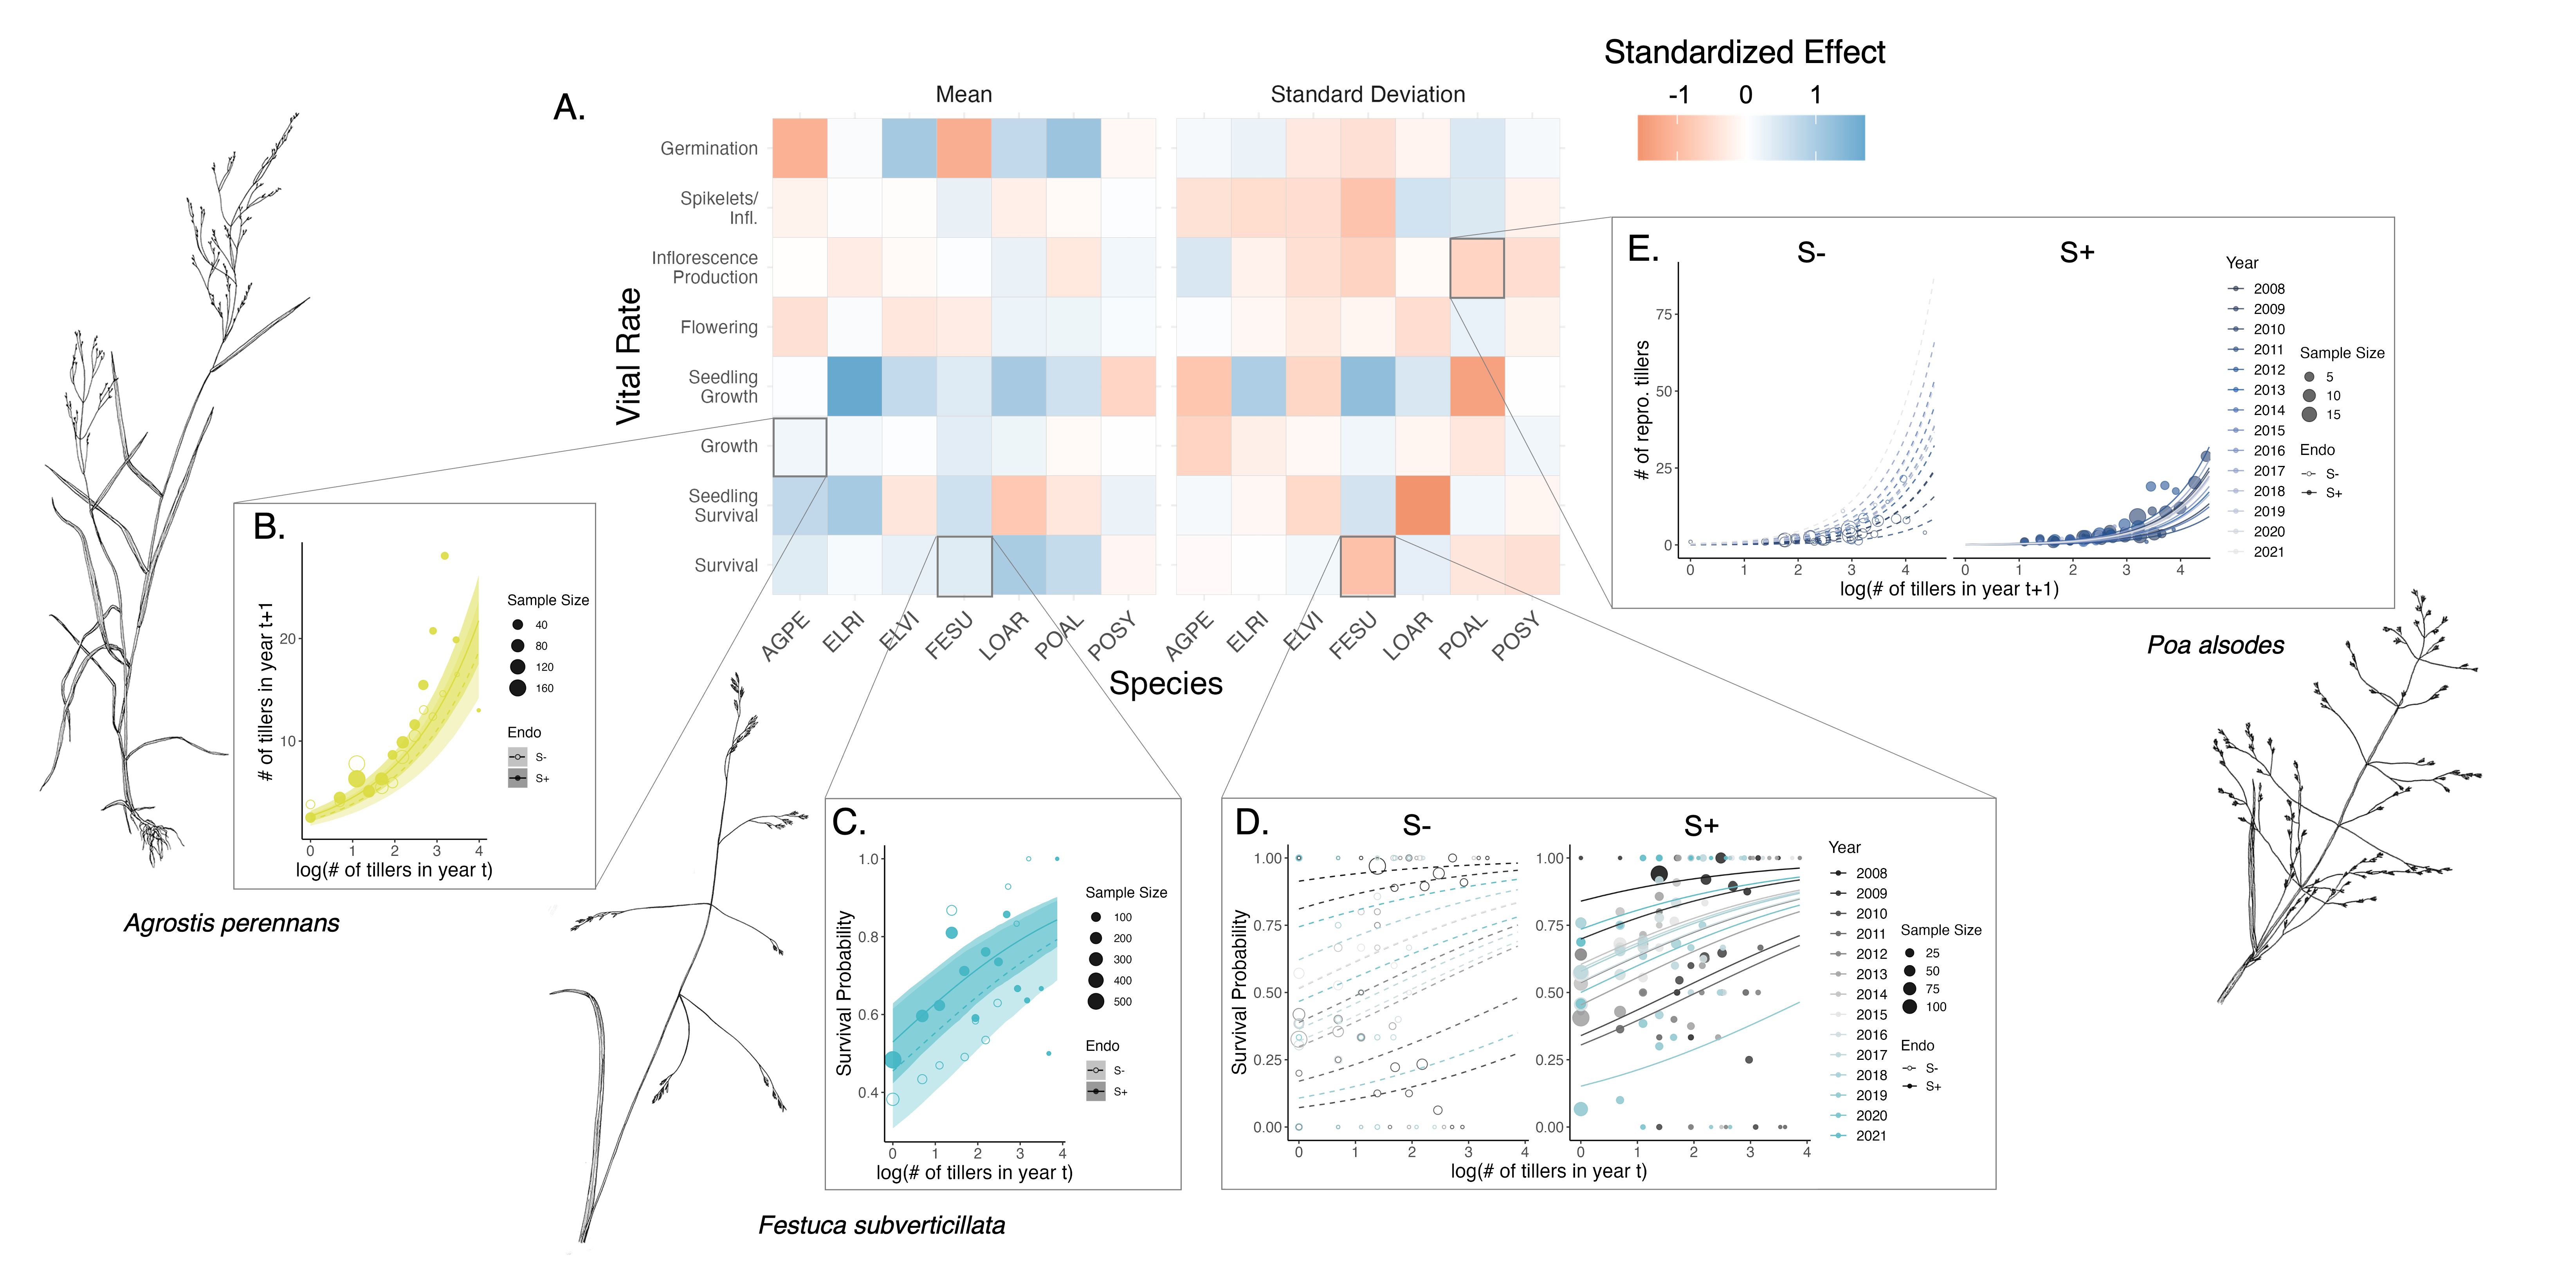
\includegraphics[width=\linewidth]{StochDemo_fig1.png}
\end{figure}
\noindent {\bf Fig. 1.} \textbf{Endophyte symbiosis altered host vital rates.} (A) Shading represents the posterior mean standardized effect size (Cohen's D) of endophyte symbiosis on mean or standard deviation of host vital rates (blue indicates that symbiosis increased the mean or standard deviation and red indicates a reduction). Endophyte presence increased (B) the mean growth rate of \emph{A. perennans} and (C) the survival probability of \emph{F. subverticillata}. Endophyte presence reduced interannual variance in (D) the survival of \emph{F. subverticillata} and (E) the fertility of \emph{P. alsodes}. Organism silhouettes modified from "Festuca subverticillata" by Cindy Roché and "Agrostis hyemalis" and "Poa alsodes" by Sandy Long © Utah State University)
\newpage

\begin{figure}
	\centering
	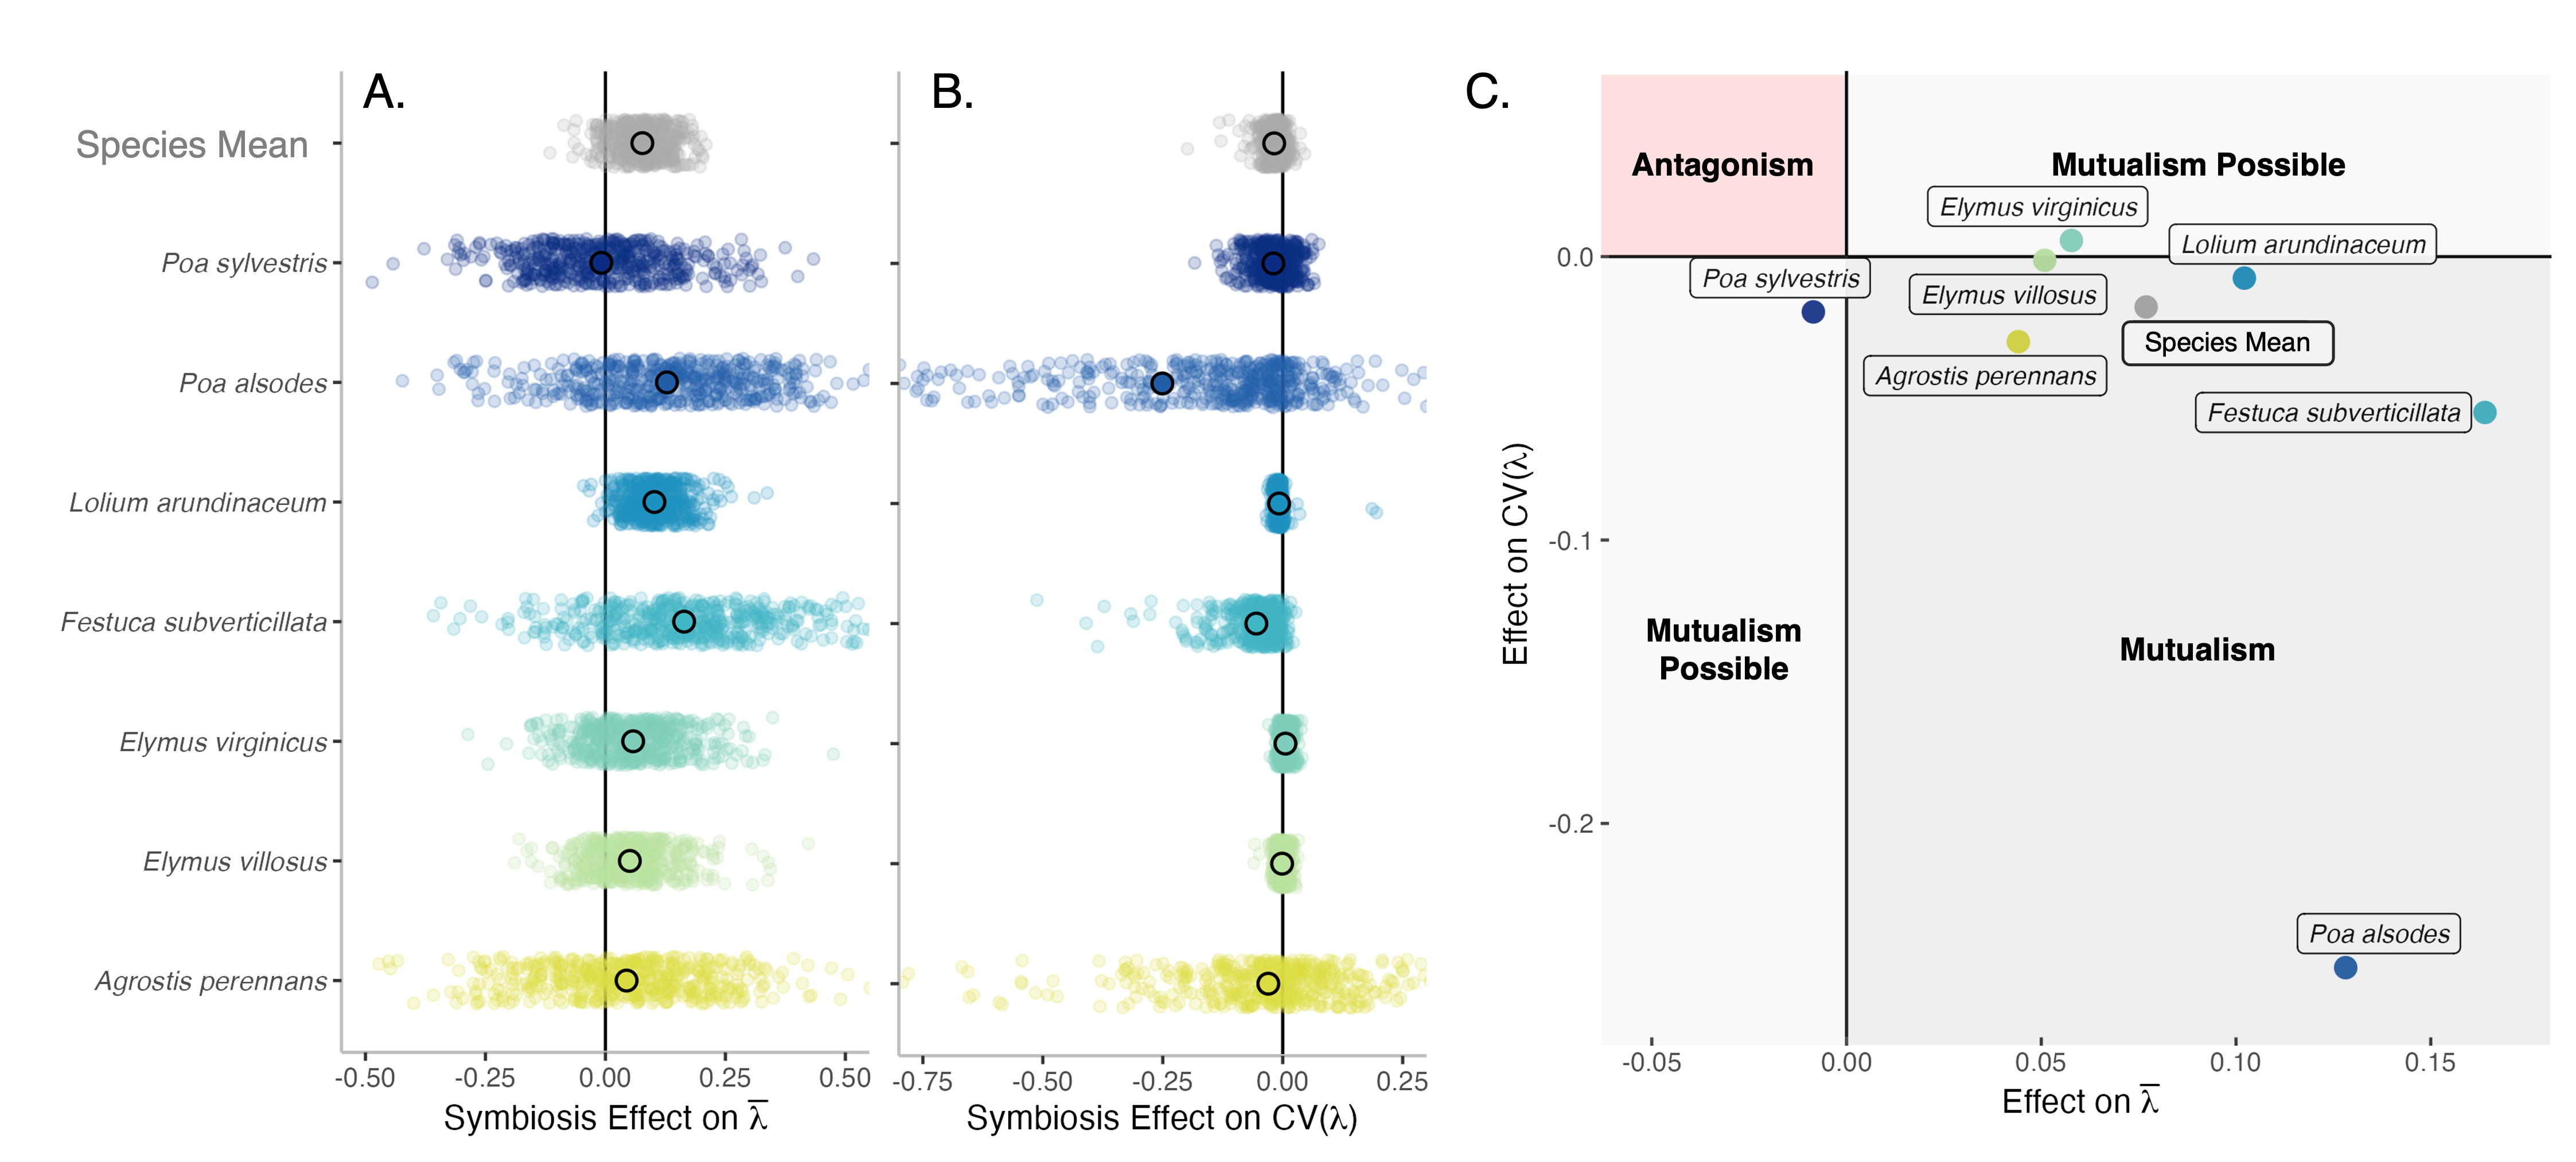
\includegraphics[width=\linewidth]{StochDemo_fig2.png}
\end{figure}
\noindent {\bf Fig. 2.} \textbf{Mean and variance-buffering effects on population growth rates.} Black circles indicate the average effect of endophytes along with 500 posterior draws (smaller colored circles) on the (A) mean and (B) coefficient of variation in population growth rates $\lambda$ for each host species as well as a cross species mean. (C) For all hosts, endophyte either reduce variance, increase the mean, or both, and consequently when considering stochastic environments, the interactions are always at least potentially mutualistic.
\newpage

\begin{figure}
	\centering
	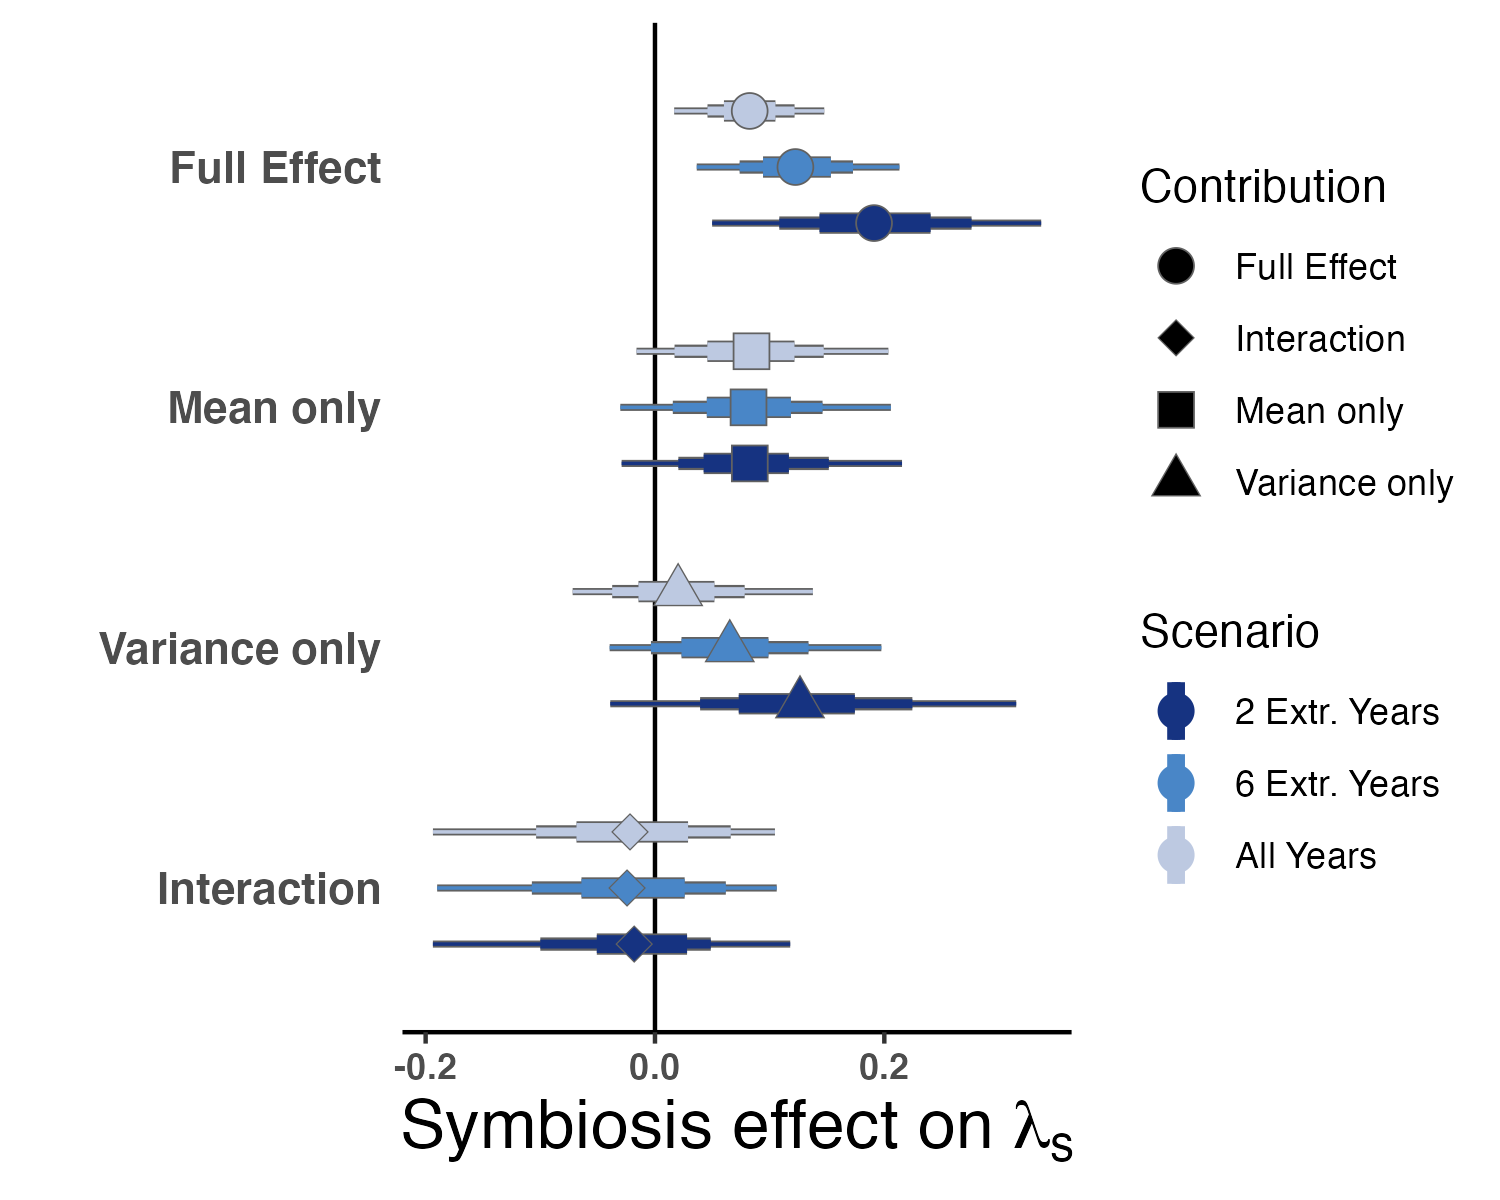
\includegraphics[width=.8\linewidth]{StochDemo_fig3.png}
\end{figure}
\noindent {\bf Fig. 3.} \textbf{Endophyte contributions to stochastic growth rates under observed and elevated variance.} Endophyte symbiosis contributes to the total effect of mutualism through benefits to mean growth rates and through variance buffering as well as the interaction between mean and variance effects. Shapes indicate the posterior mean of each contribution averaged across the seven focal symbiota, along with bars for the 50, 75 and 95 \% credible intervals.  The full effect of the symbiosis (circles) becomes more mutualistic under scenarios of increased variance (represented by color intensity). Relative to a scenario sampling transition matrices for all 14 years during the study period, simulations increased variance by sampling the most extreme six or two years, leading to increased contributions from variance buffering effects (triangles) and a constant contribution from mean effects (squares).
\newpage


\begin{figure}
	\centering
	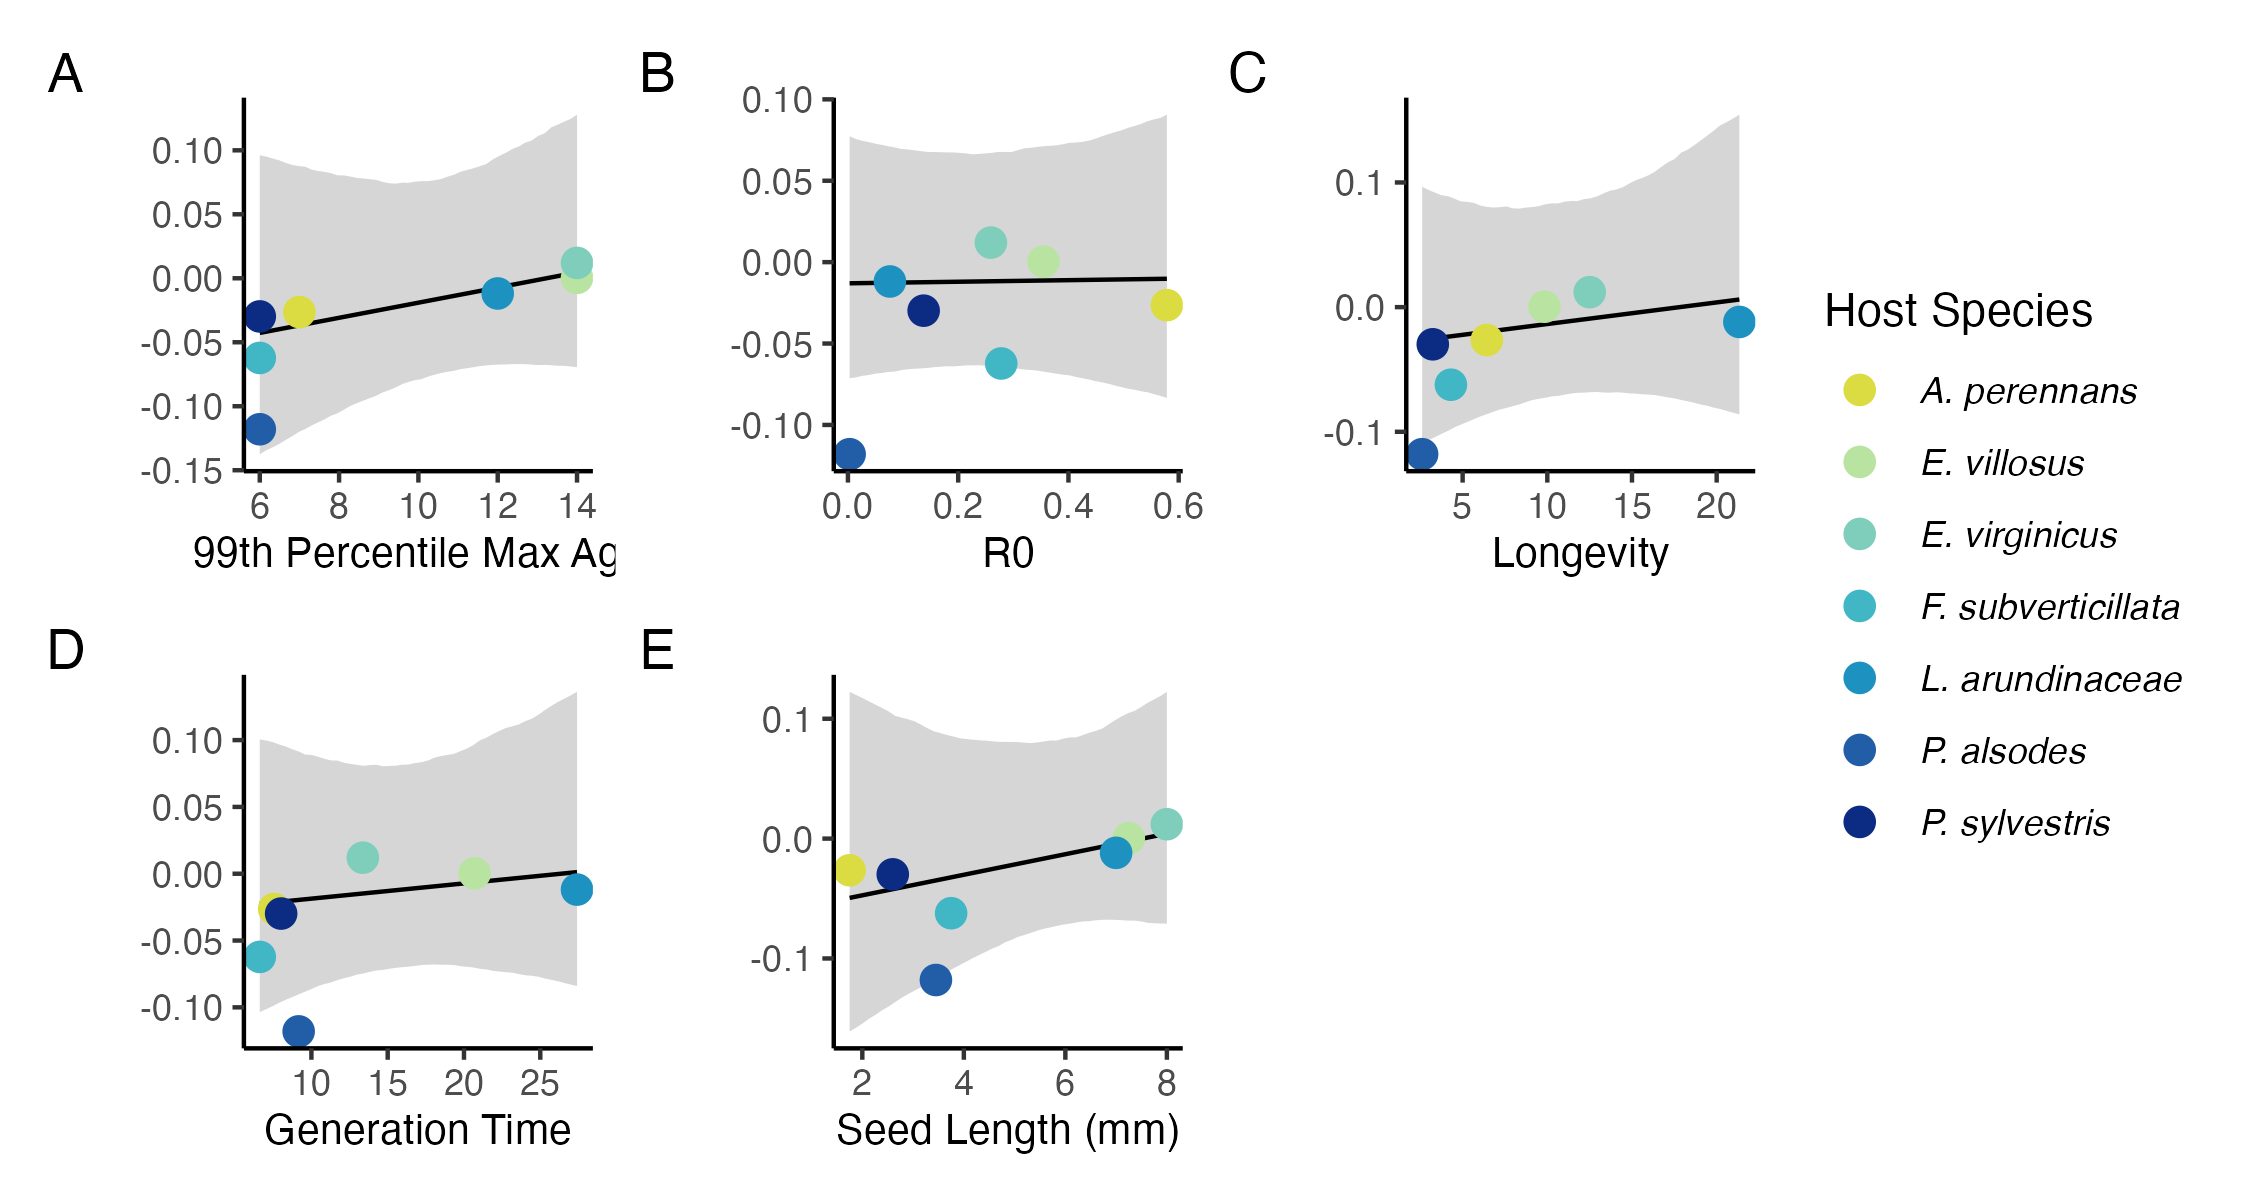
\includegraphics[width=\linewidth]{StochDemo_fig4.png}
\end{figure}
\noindent {\bf Fig. 4.} \textbf{Host species with faster life history traits experience stronger effects of symbiont-mediated variance buffering.} Regressions between life history traits describing the fast-slow life history continuum ((A) Maximum age observed during long term censuses; (B) 99th percentile maximum age during demographic censuses; (C) Net reproductive rate; (D) Longevity; (E) Mean life expectancy; (F) Generation time; (G) Seed size; (H) Rate of imperfect transmission) and the effect of endophyte symbiosis on the coefficent of variation in population growth rate ($\lambda$). Each panel shows the fitted mean relationship (line) along with with the 95\% credible interval.
\newpage


\begin{figure}[H]
	\centering
	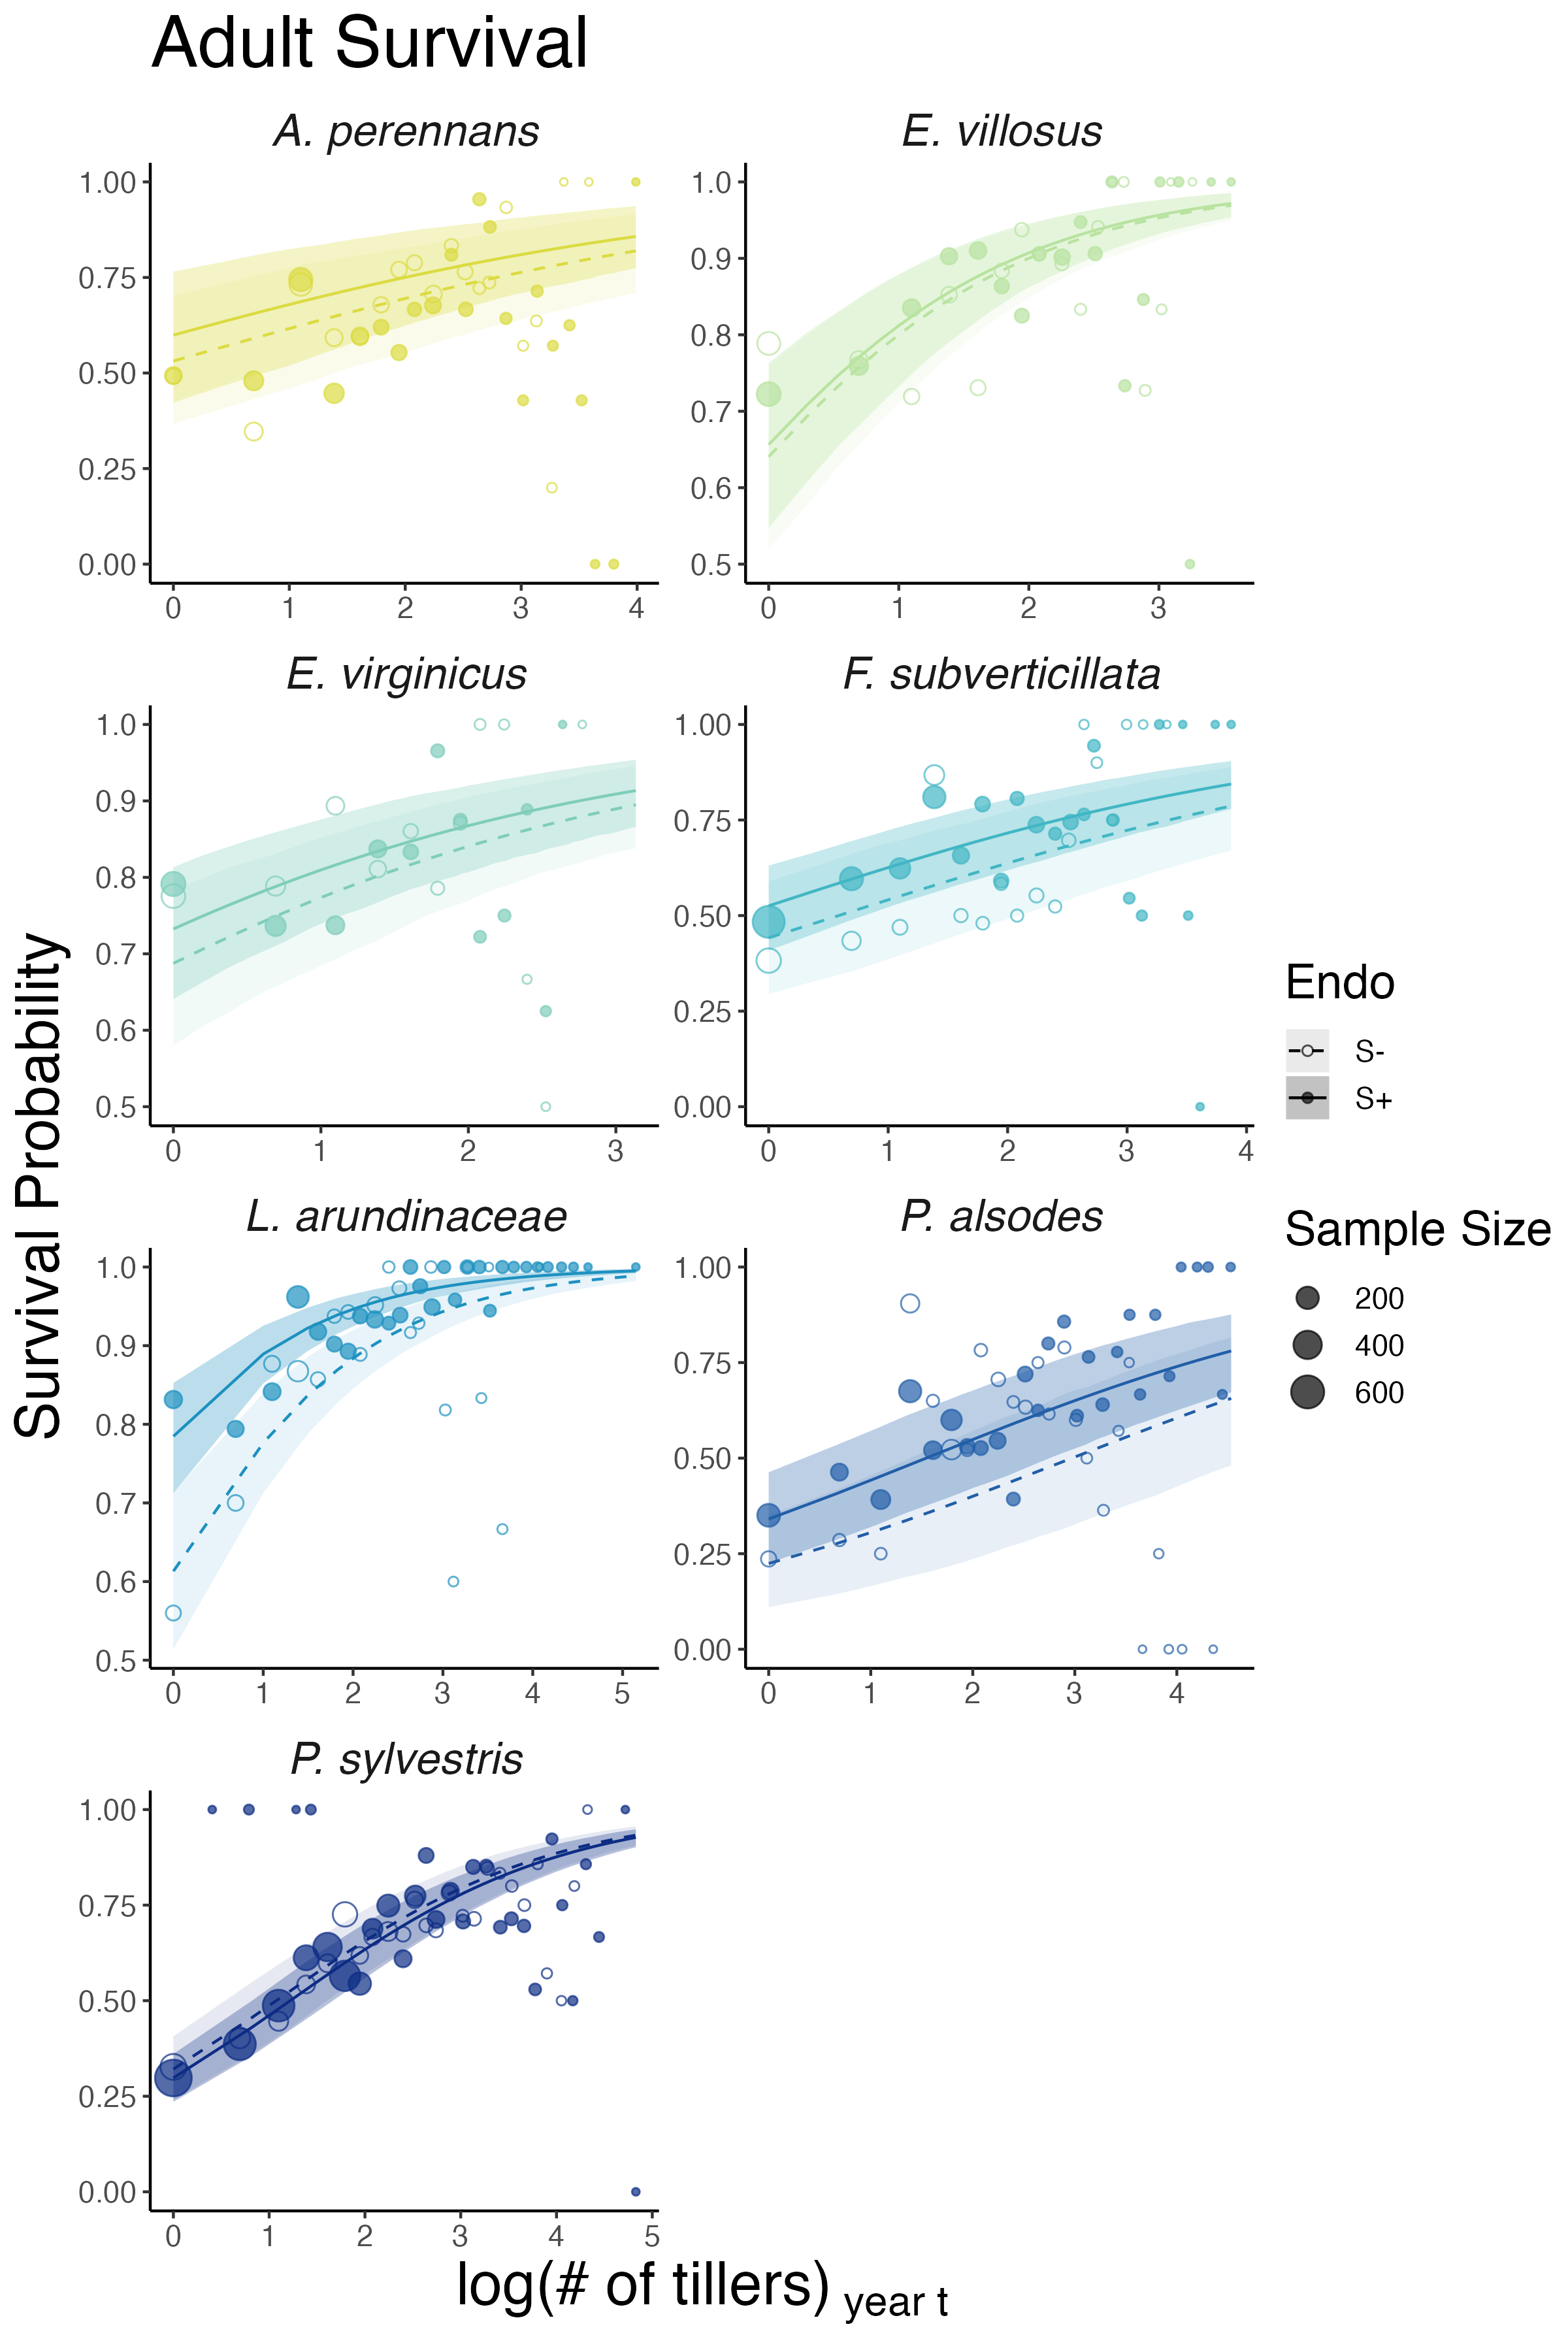
\includegraphics[width=.8\linewidth]{surv_meanplot.png}
\end{figure}
\noindent {\bf Fig. S1.} \textbf{Effect of endophyte symbiosis on the mean value of adult survival.} Fitted curves represent the size-specific mean survival probability along with data binned by size shown as open circles with a dashed line for symbiont-free (S-) plants , while the solid line and filled circles represent symbiontic (S+) plants. 80\% credible intervals are shown with dark shading for  S+, or light shading for S-.
\begin{figure}[H]
	\centering
	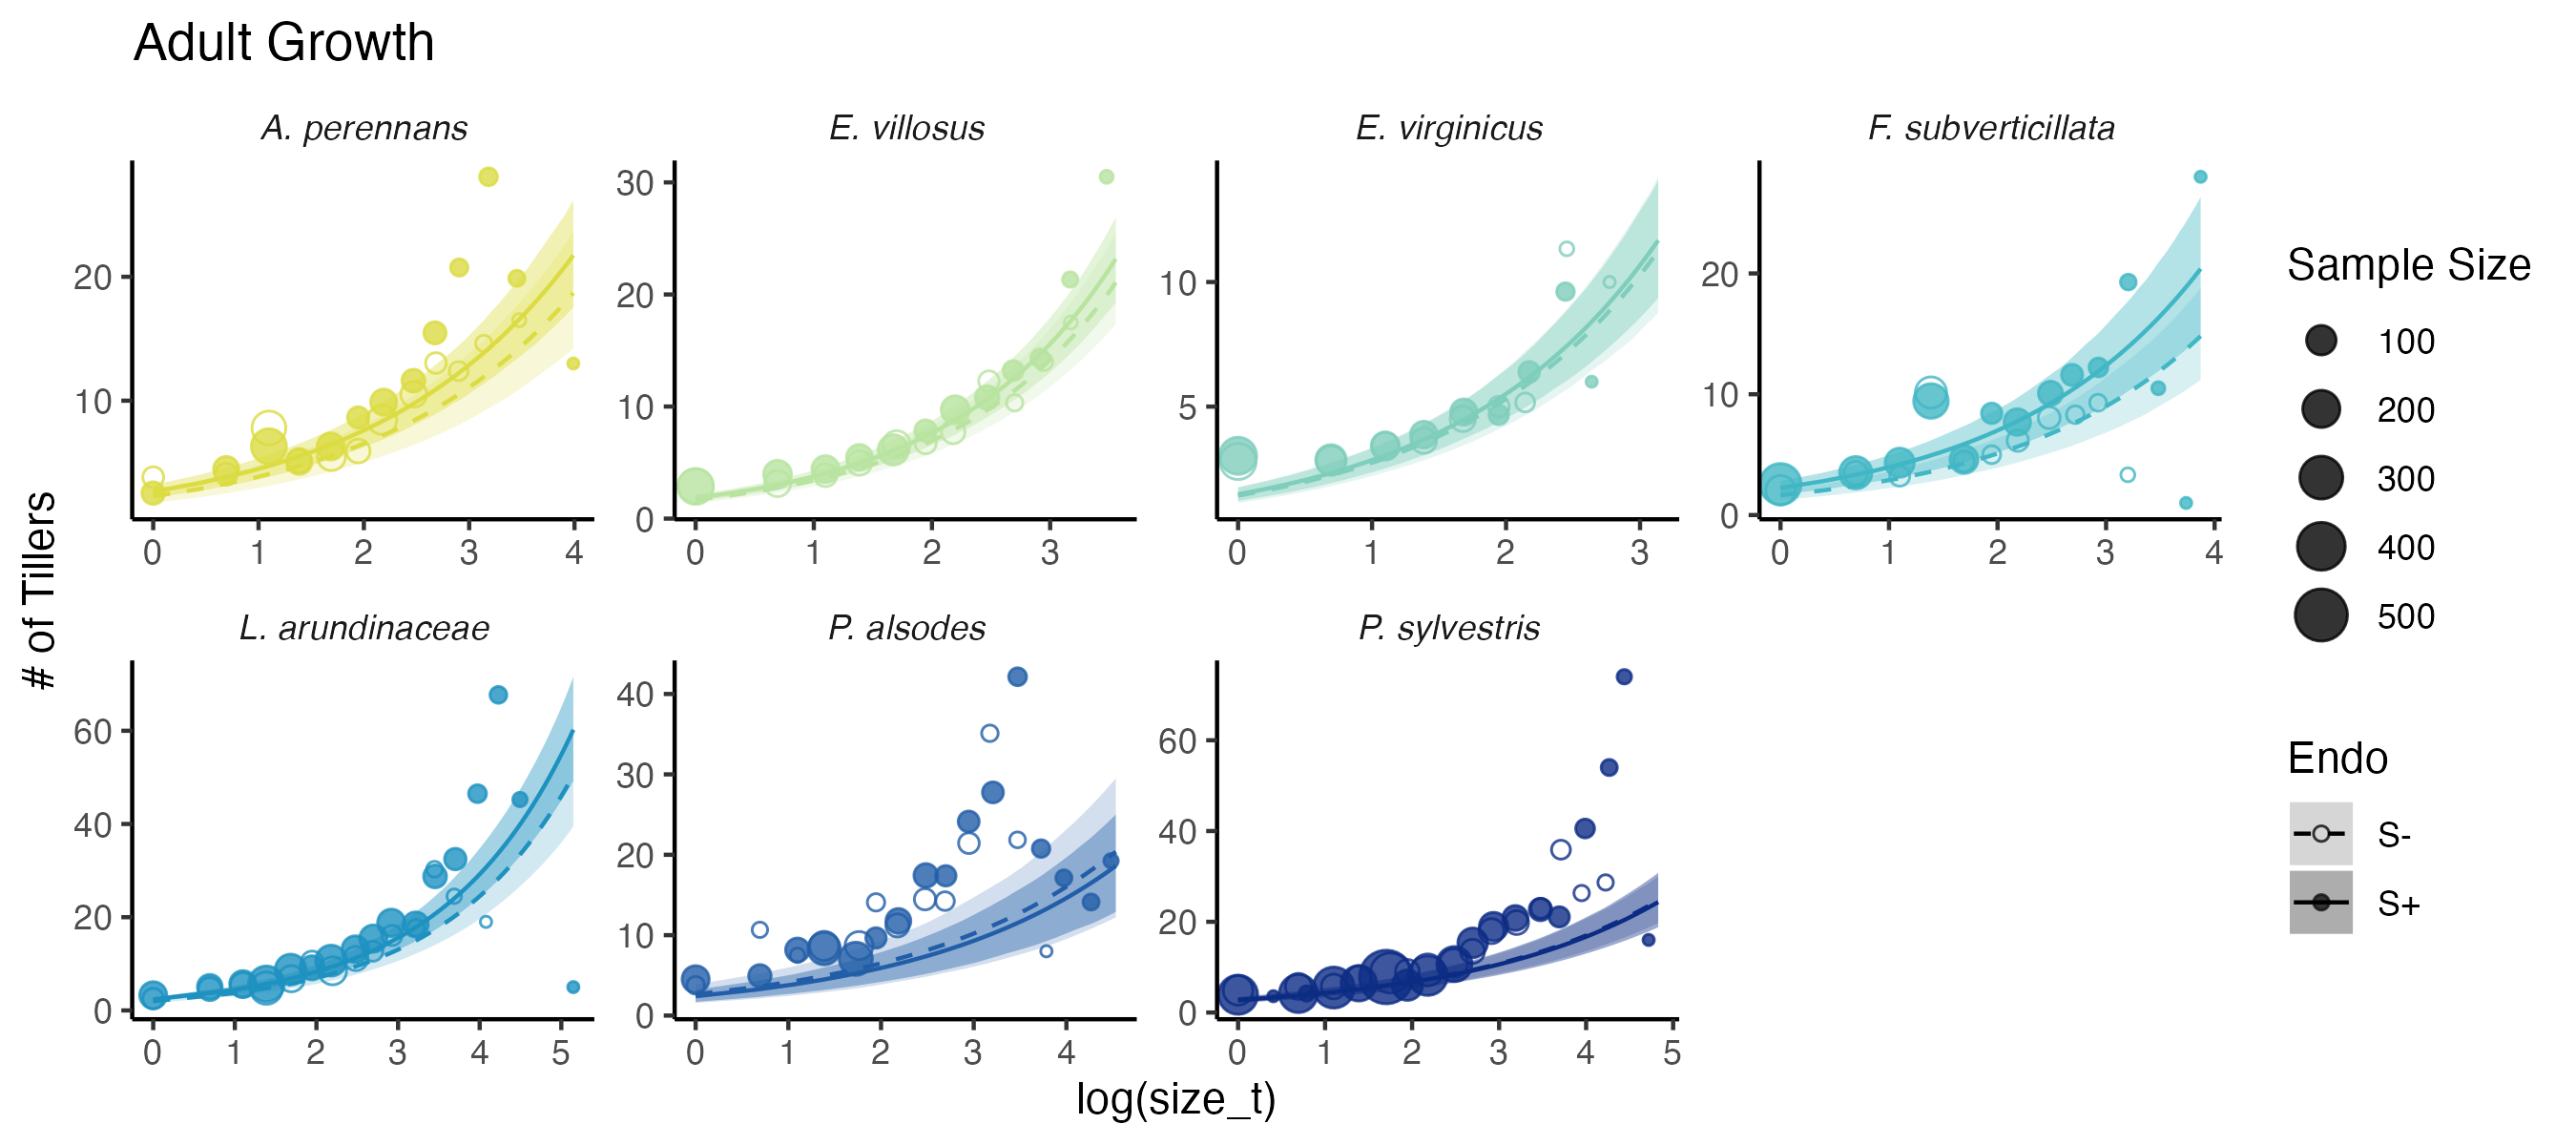
\includegraphics[width=.8\linewidth]{grow_meanplot.png}
\end{figure}
\noindent {\bf Fig. S2.} \textbf{Effect of endophyte symbiosis on the mean value of adult growth.} Fitted curves represent the size-specific mean expected plant size along with data binned by size shown as open circles with a dashed line for symbiont-free (S-) plants , while the solid line and filled circles represent symbiontic (S+) plants. 80\% credible intervals are shown with dark shading for  S+, or light shading for S-.
\newpage

\begin{figure}[H]
	\centering
	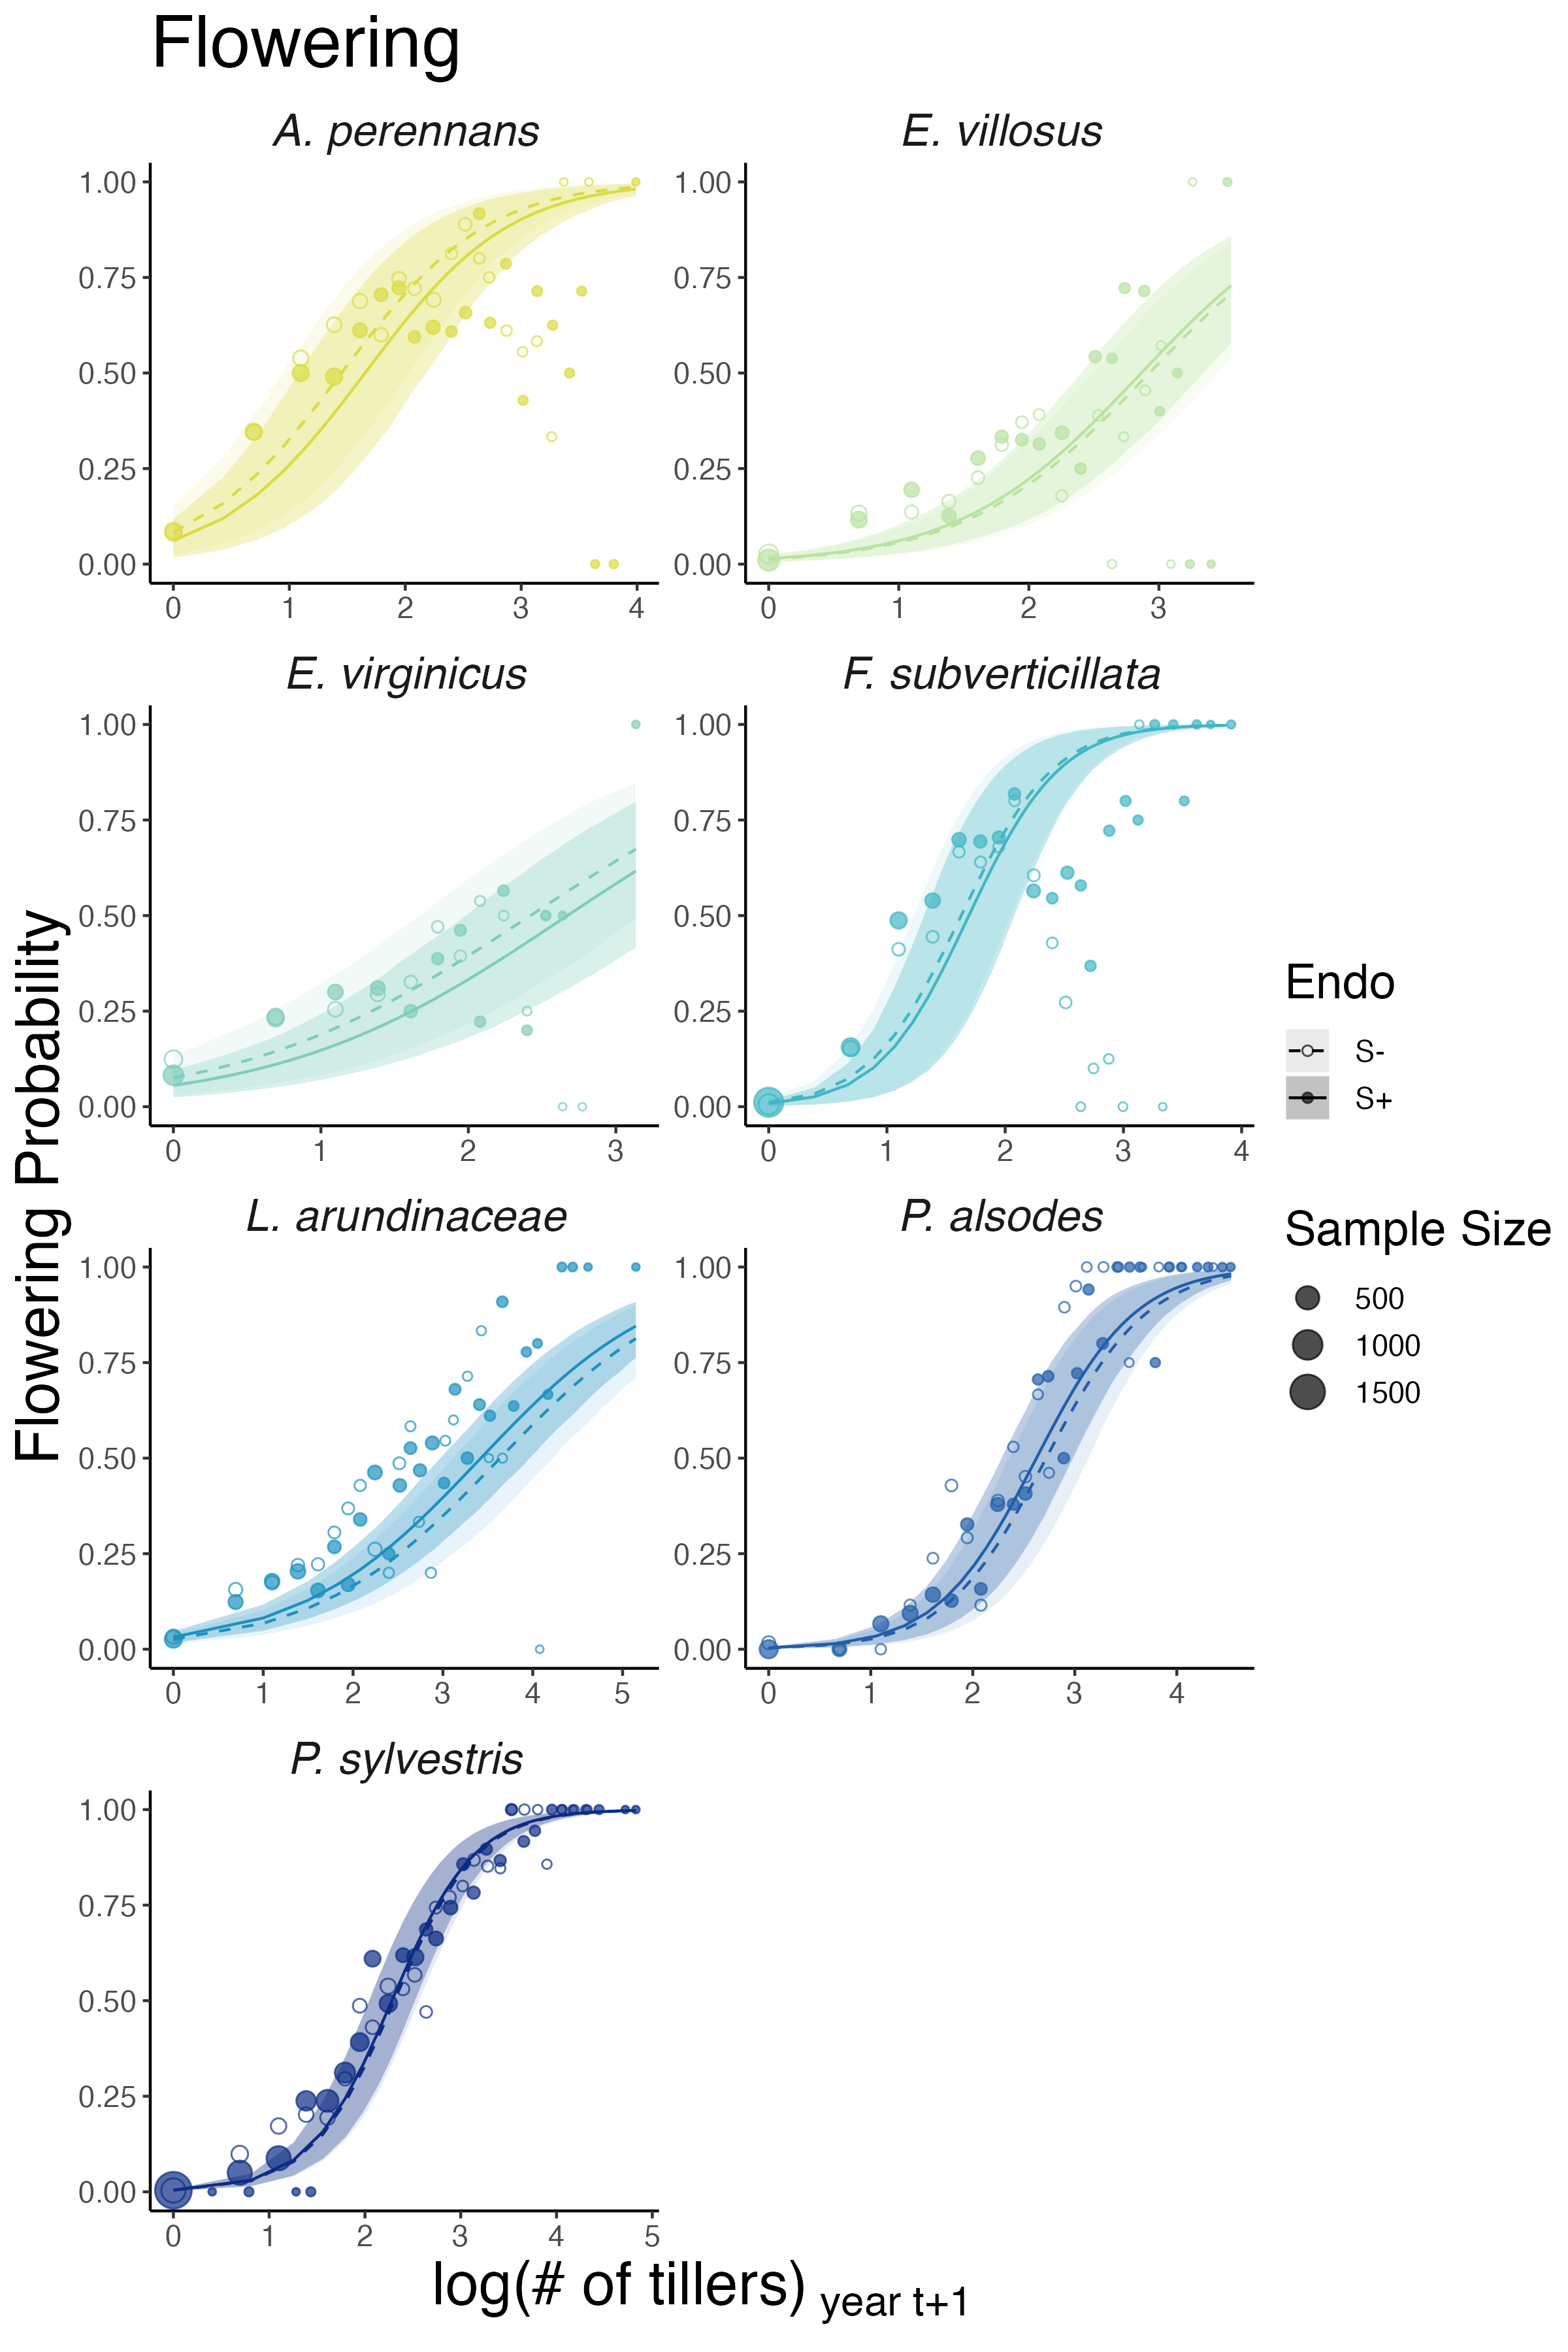
\includegraphics[width=.8\linewidth]{flw_meanplot.png}
\end{figure}
\noindent {\bf Fig. S3.} \textbf{Effect of endophyte symbiosis on the mean value of flowering} Fitted curves represent the size-specific mean flowering probability along with data binned by size shown as open circles with a dashed line for symbiont-free (S-) plants , while the solid line and filled circles represent symbiontic (S+) plants. 80\% credible intervals are shown with dark shading for  S+, or light shading for S-.
\begin{figure}[H]
	\centering
	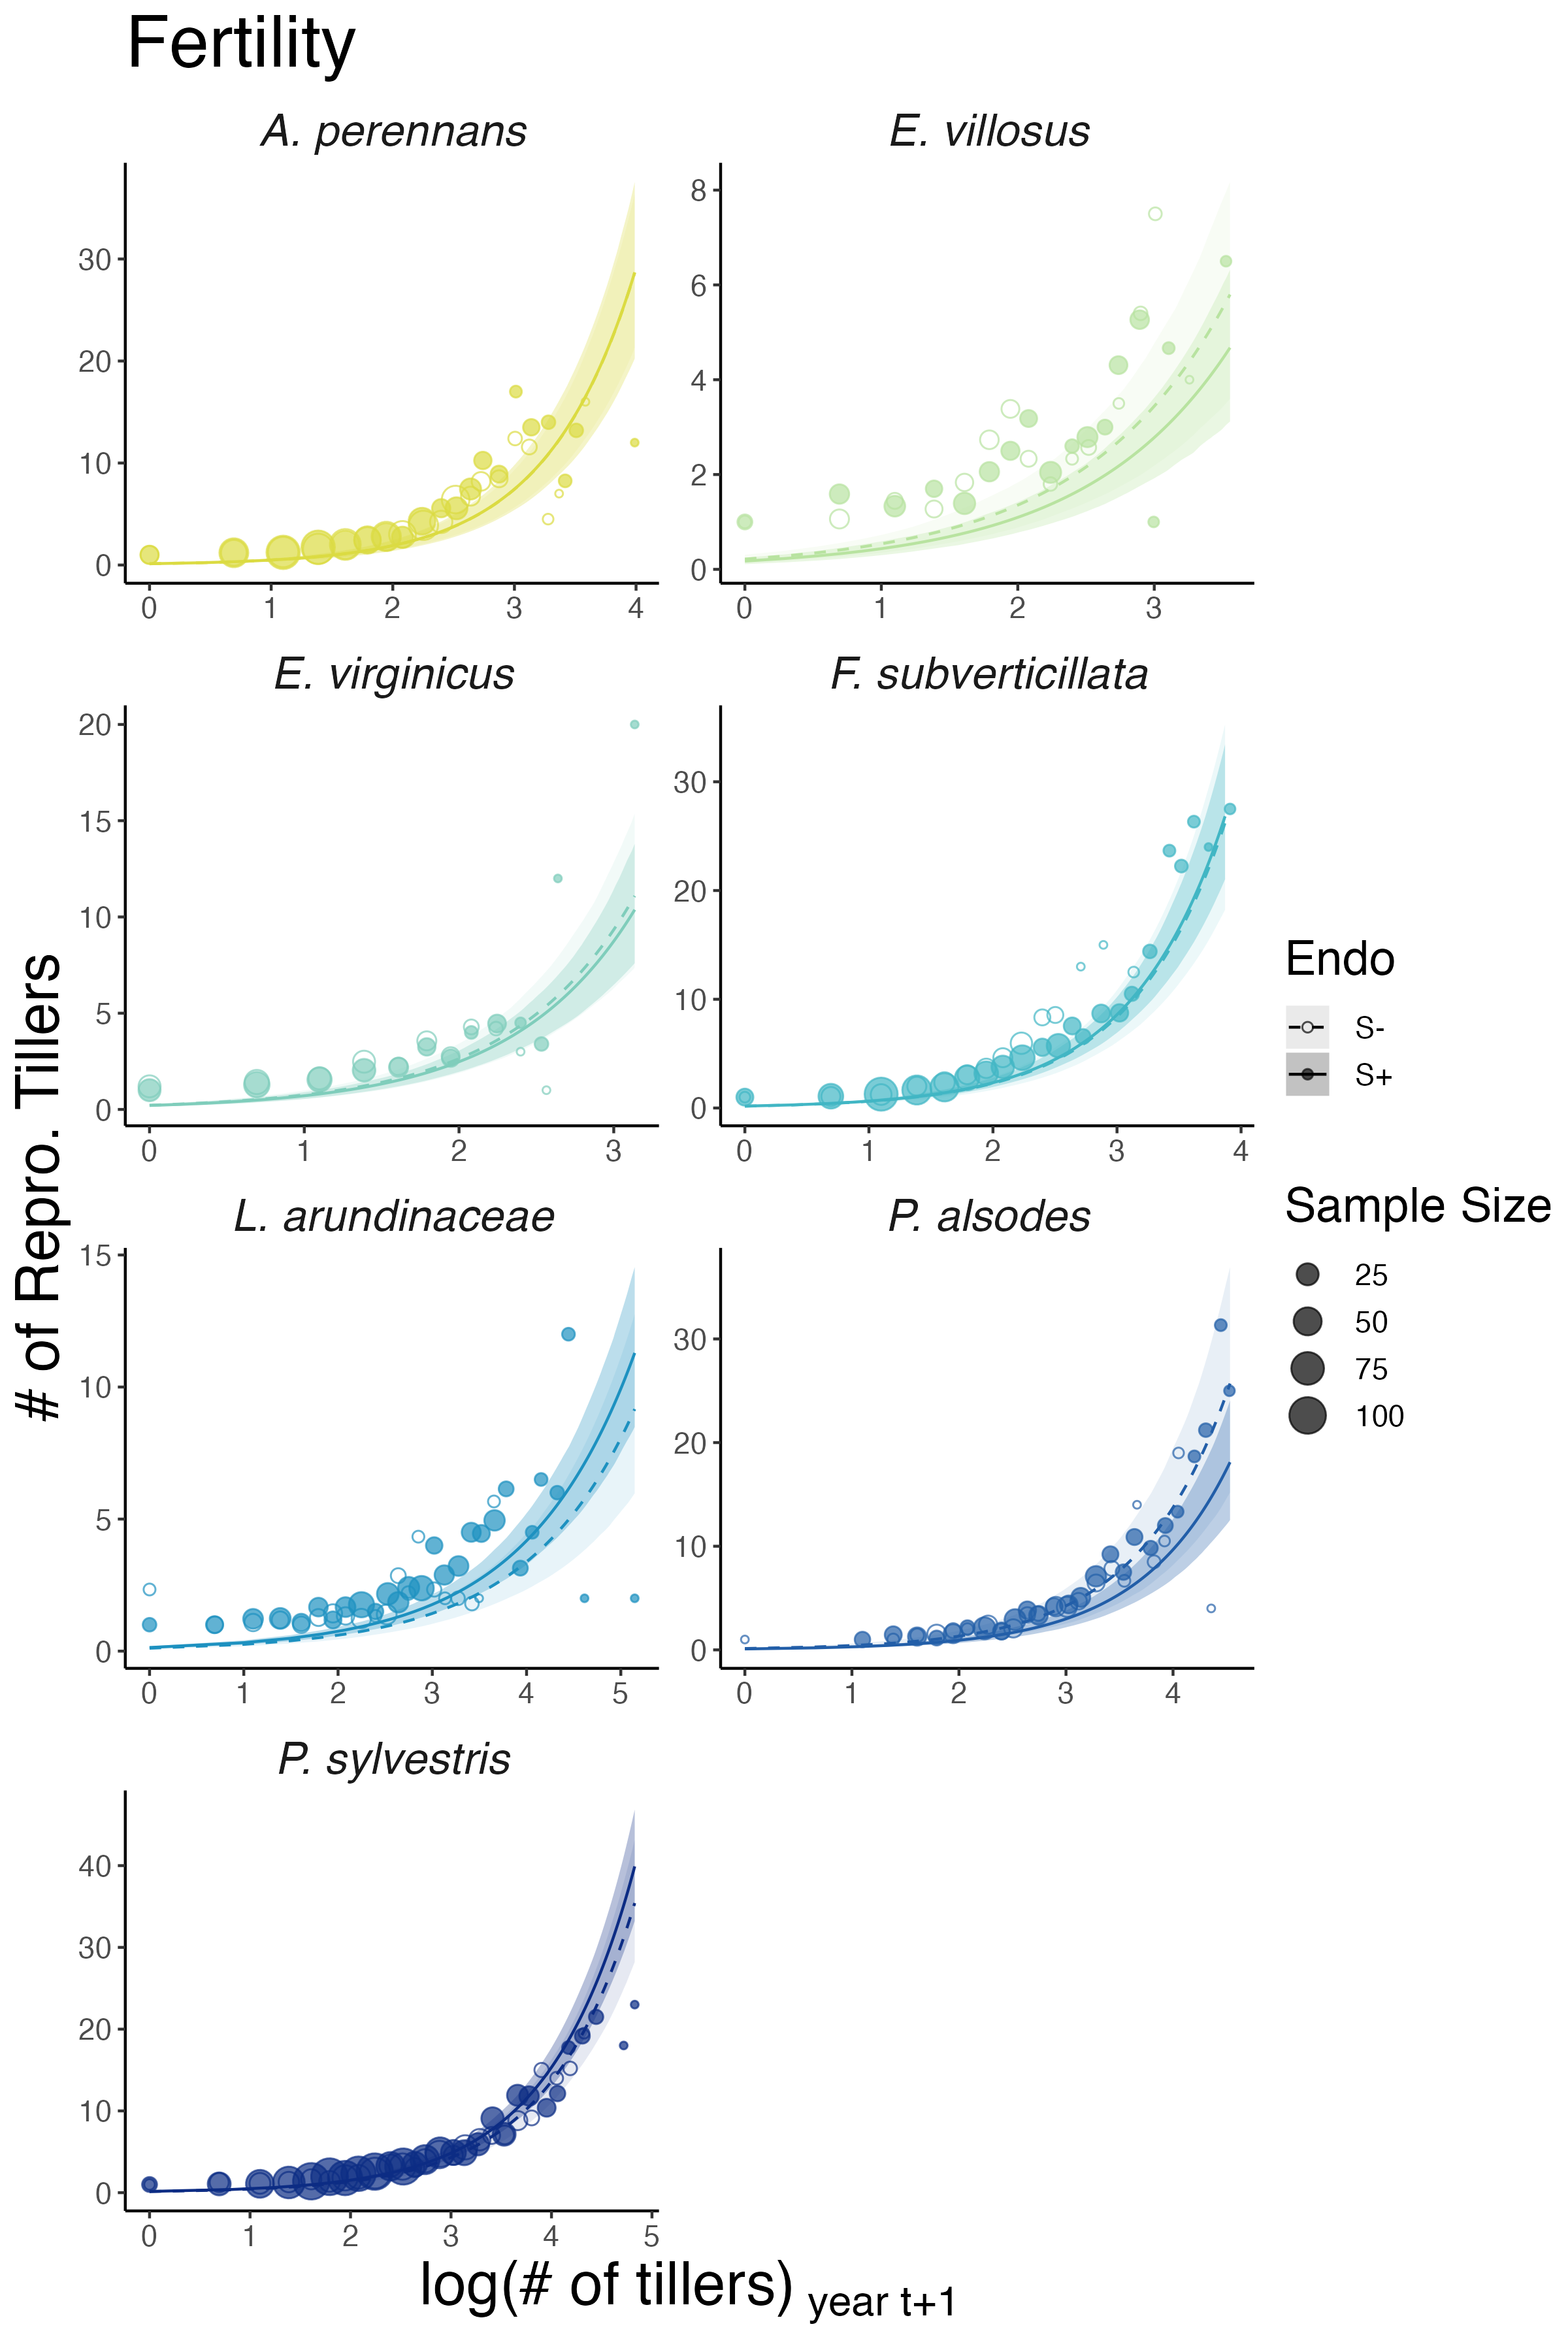
\includegraphics[width=.8\linewidth]{fert_meanplot.png}
\end{figure}
\noindent {\bf Fig. S4.} \textbf{Effect of endophyte symbiosis on the mean value of fertility.} Fitted curves represent the size-specific mean expected number of flowering tillers along with data binned by size shown as open circles with a dashed line for symbiont-free (S-) plants , while the solid line and filled circles represent symbiontic (S+) plants. 80\% credible intervals are shown with dark shading for  S+, or light shading for S-.
\newpage
\begin{figure}[H]
	\centering
	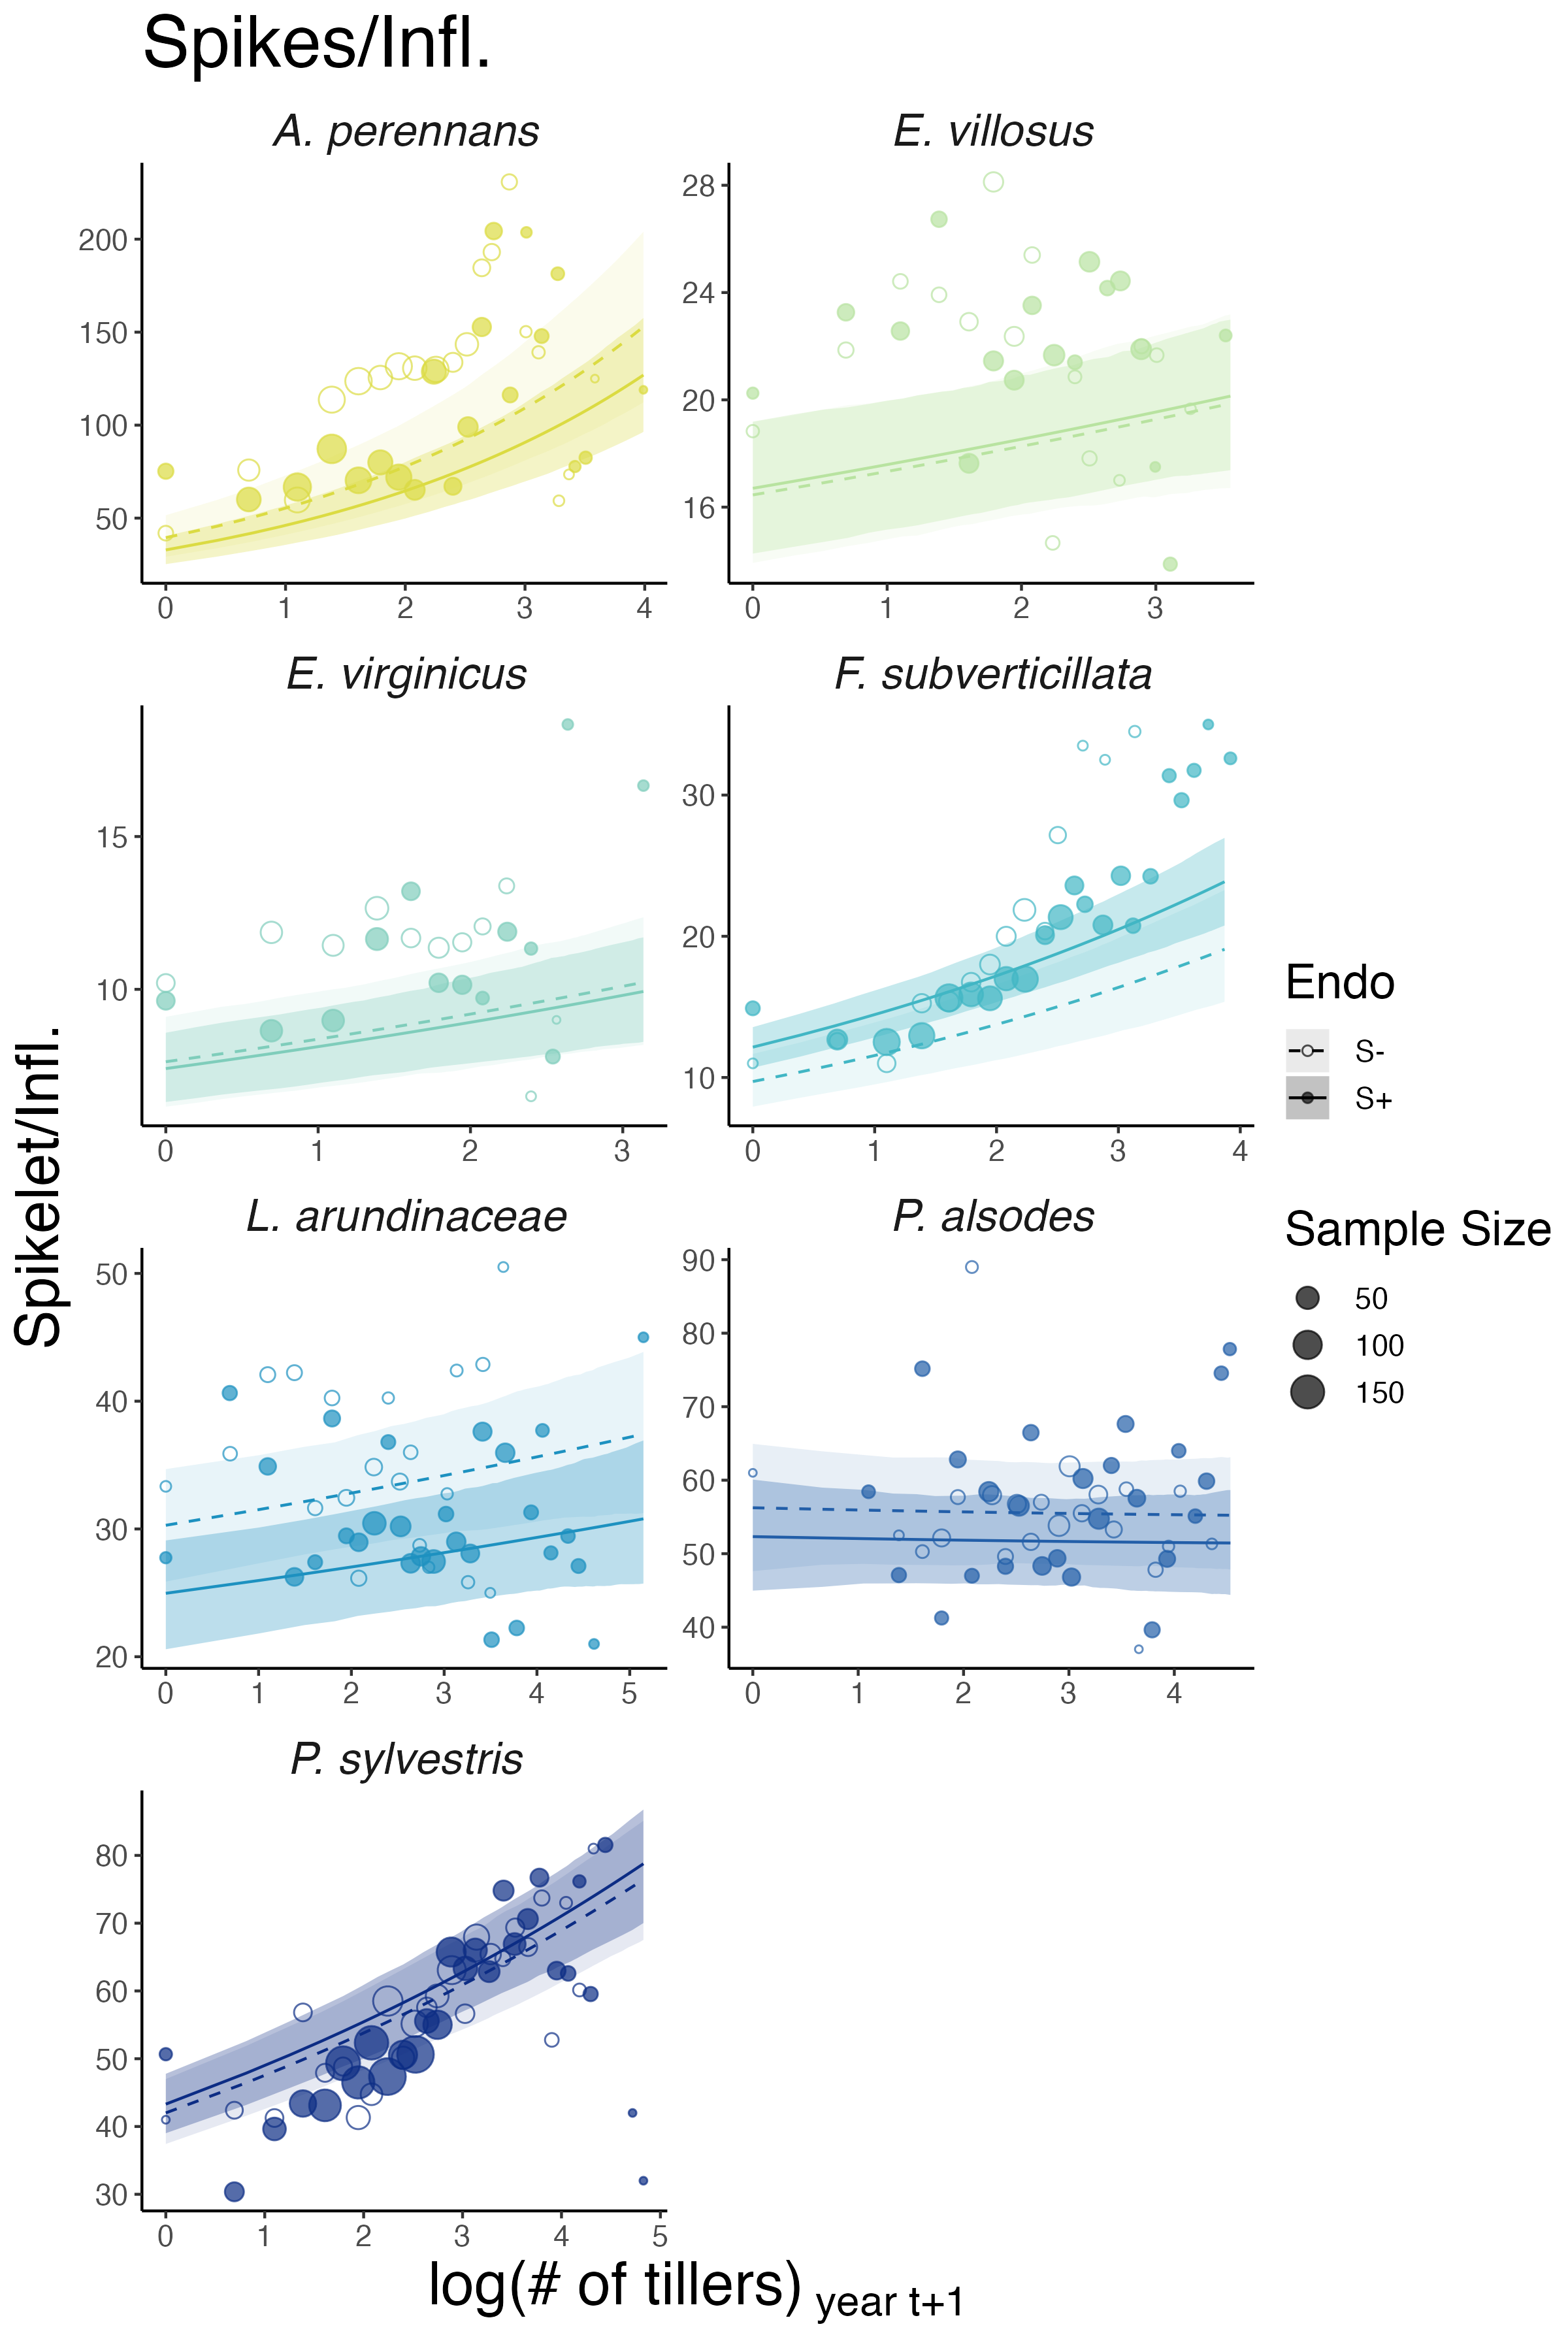
\includegraphics[width=.8\linewidth]{spike_meanplot.png}
\end{figure}
\noindent {\bf Fig. S5.} \textbf{Effect of endophyte symbiosis on the mean value of spikelet production.} Fitted curves represent the size-specific mean expected number of spikelets per inflorescence along with data binned by size shown as open circles with a dashed line for symbiont-free (S-) plants , while the solid line and filled circles represent symbiontic (S+) plants. 80\% credible intervals are shown with dark shading for  S+, or light shading for S-.
\newpage



\begin{figure}[H]
	\centering
	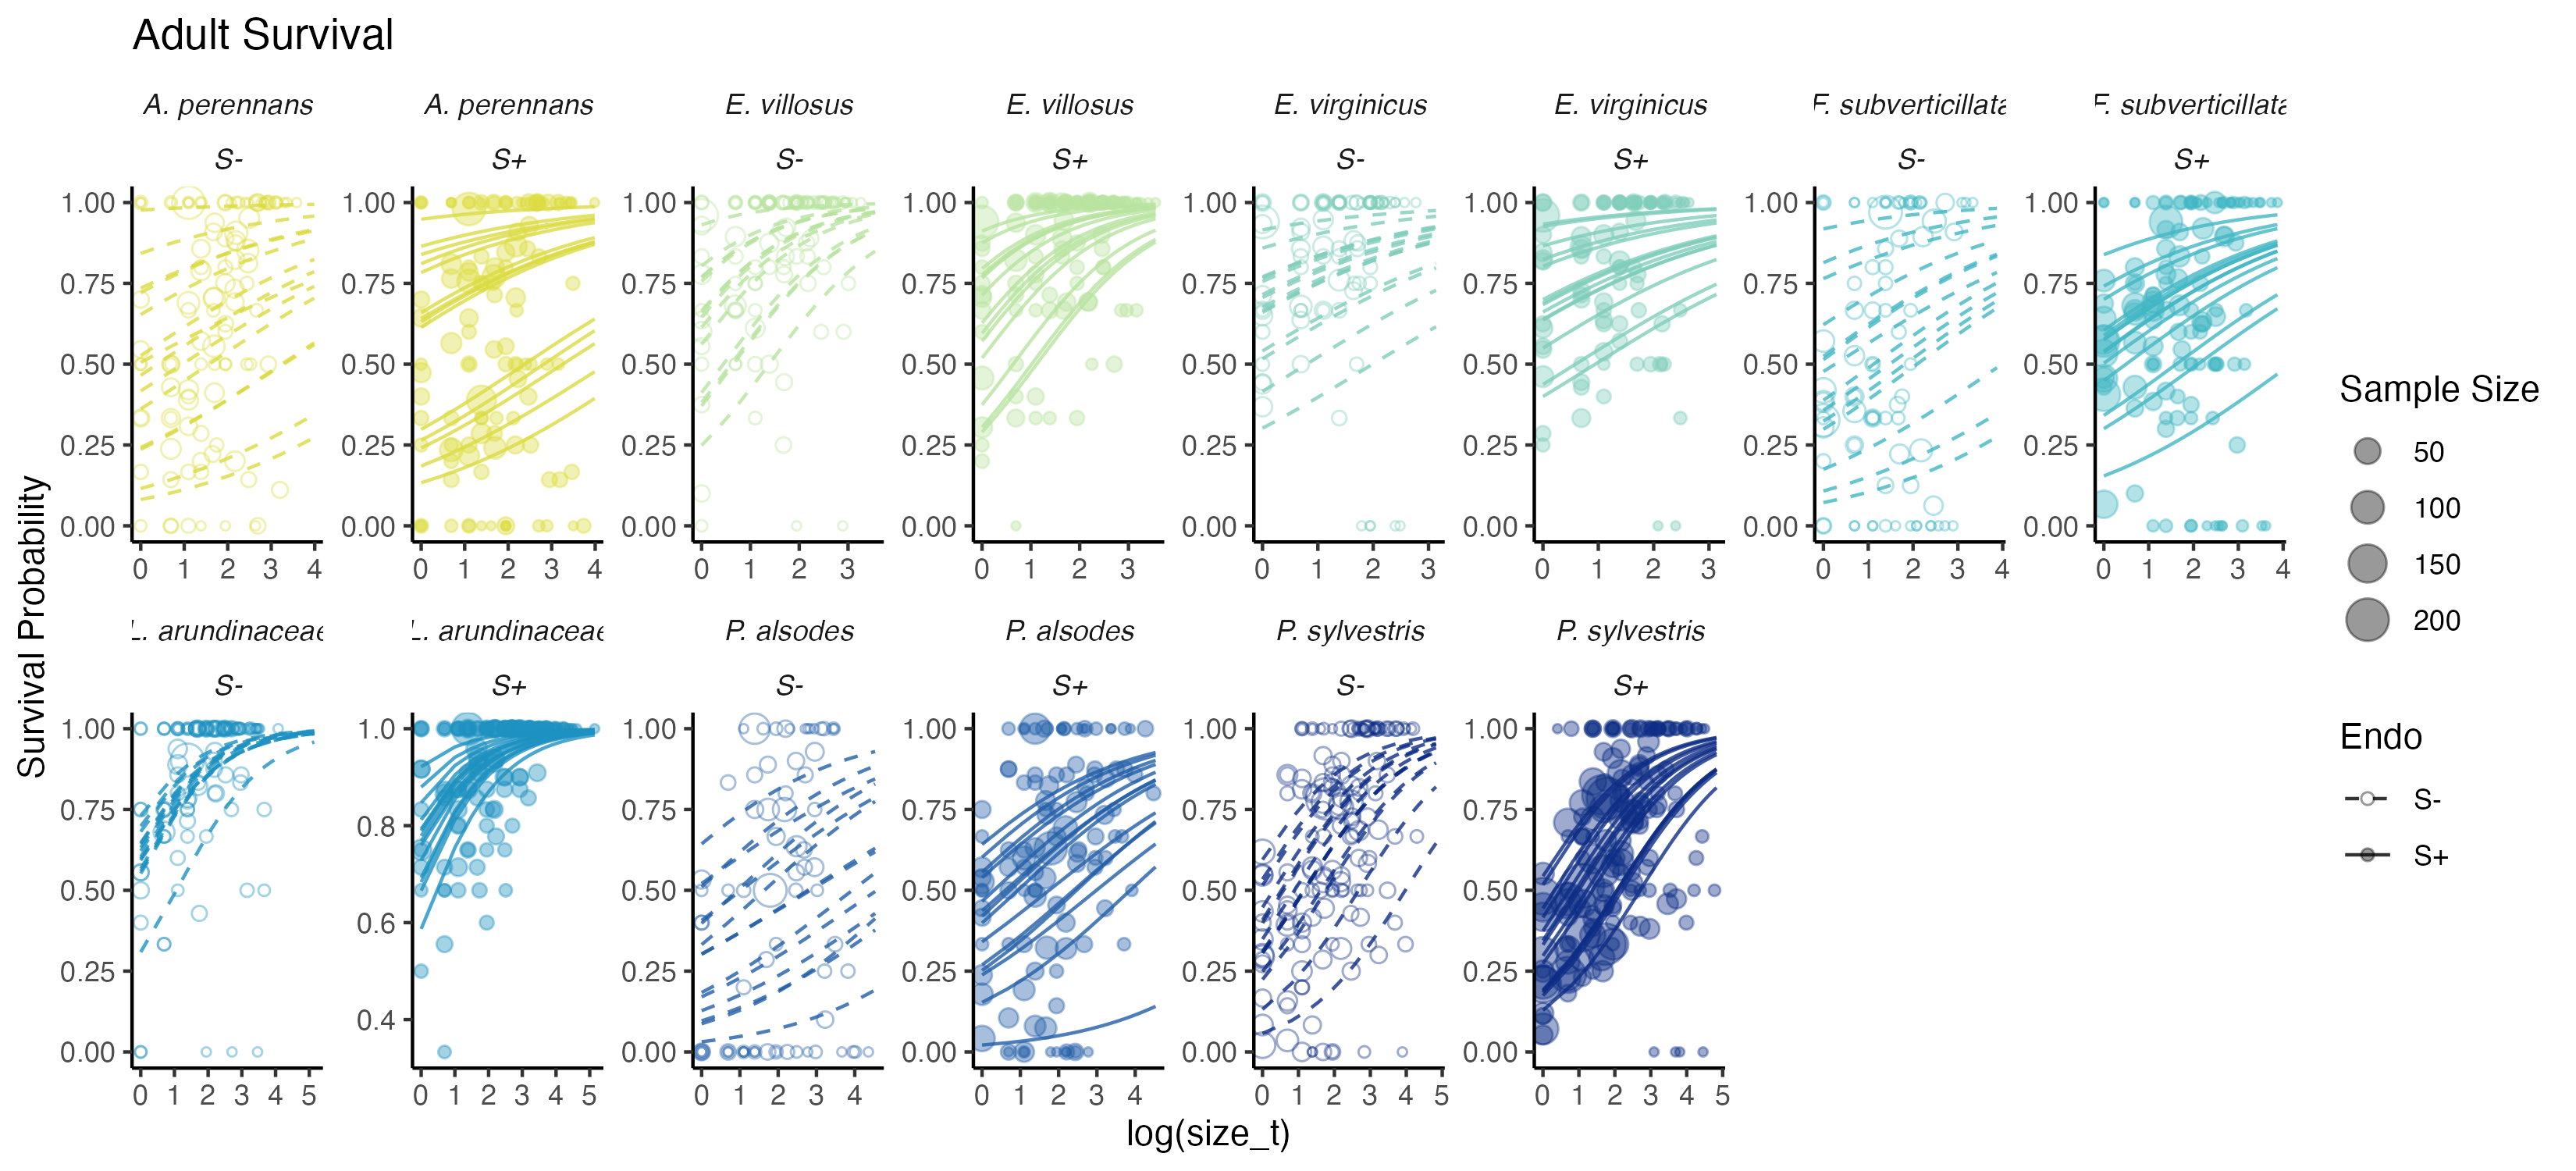
\includegraphics[width=.8\linewidth]{surv_yearplot.png}
\end{figure}
\noindent {\bf Fig. S6.} \textbf{Effect of endophyte symbiosis on yearly adult survival.} Fitted curves represent the size-specific annual survival probability along with data binned by size shown as open circles with a dashed line for symbiont-free (S-) plants , while the solid line and filled circles represent symbiontic (S+) plants. 
\begin{figure}[H]
	\centering
	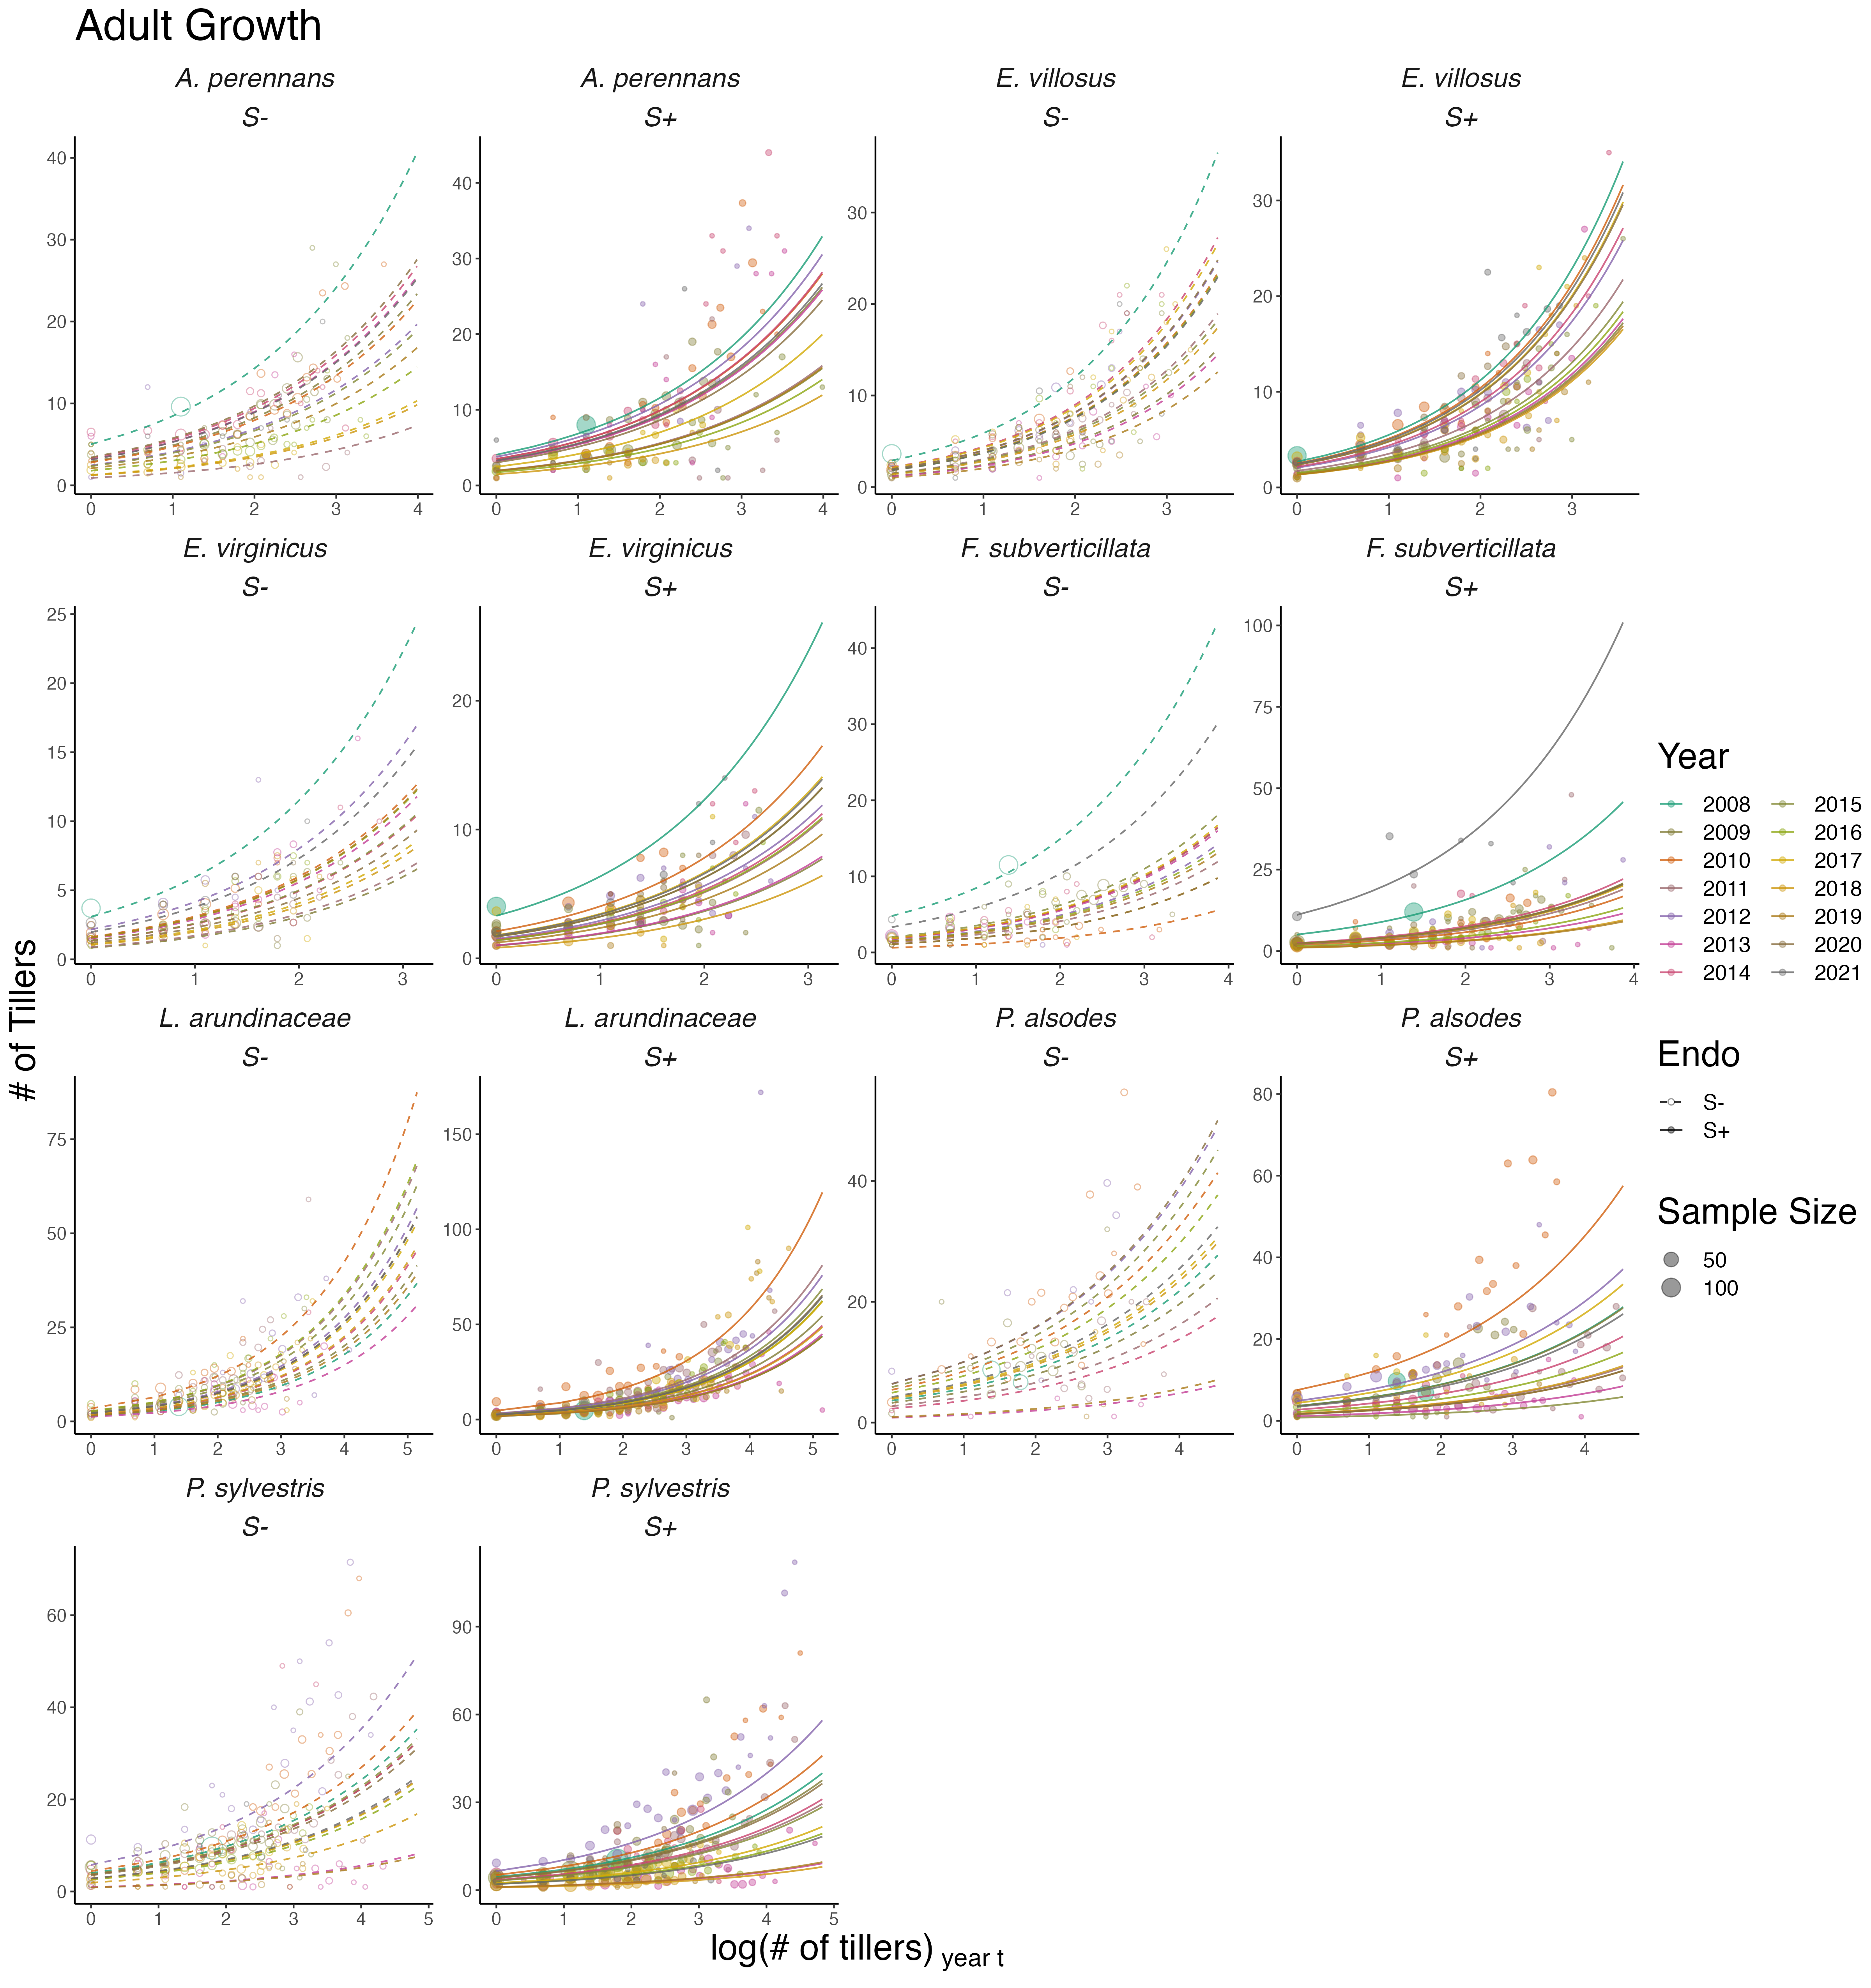
\includegraphics[width=.8\linewidth]{grow_yearplot.png}
\end{figure}
\noindent {\bf Fig. S7.} \textbf{Effect of endophyte symbiosis on yearly adult growth.} Fitted curves represent the size-specific annual expected plant size along with data binned by size shown as open circles with a dashed line for symbiont-free (S-) plants , while the solid line and filled circles represent symbiontic (S+) plants. 
\newpage

\begin{figure}[H]
	\centering
	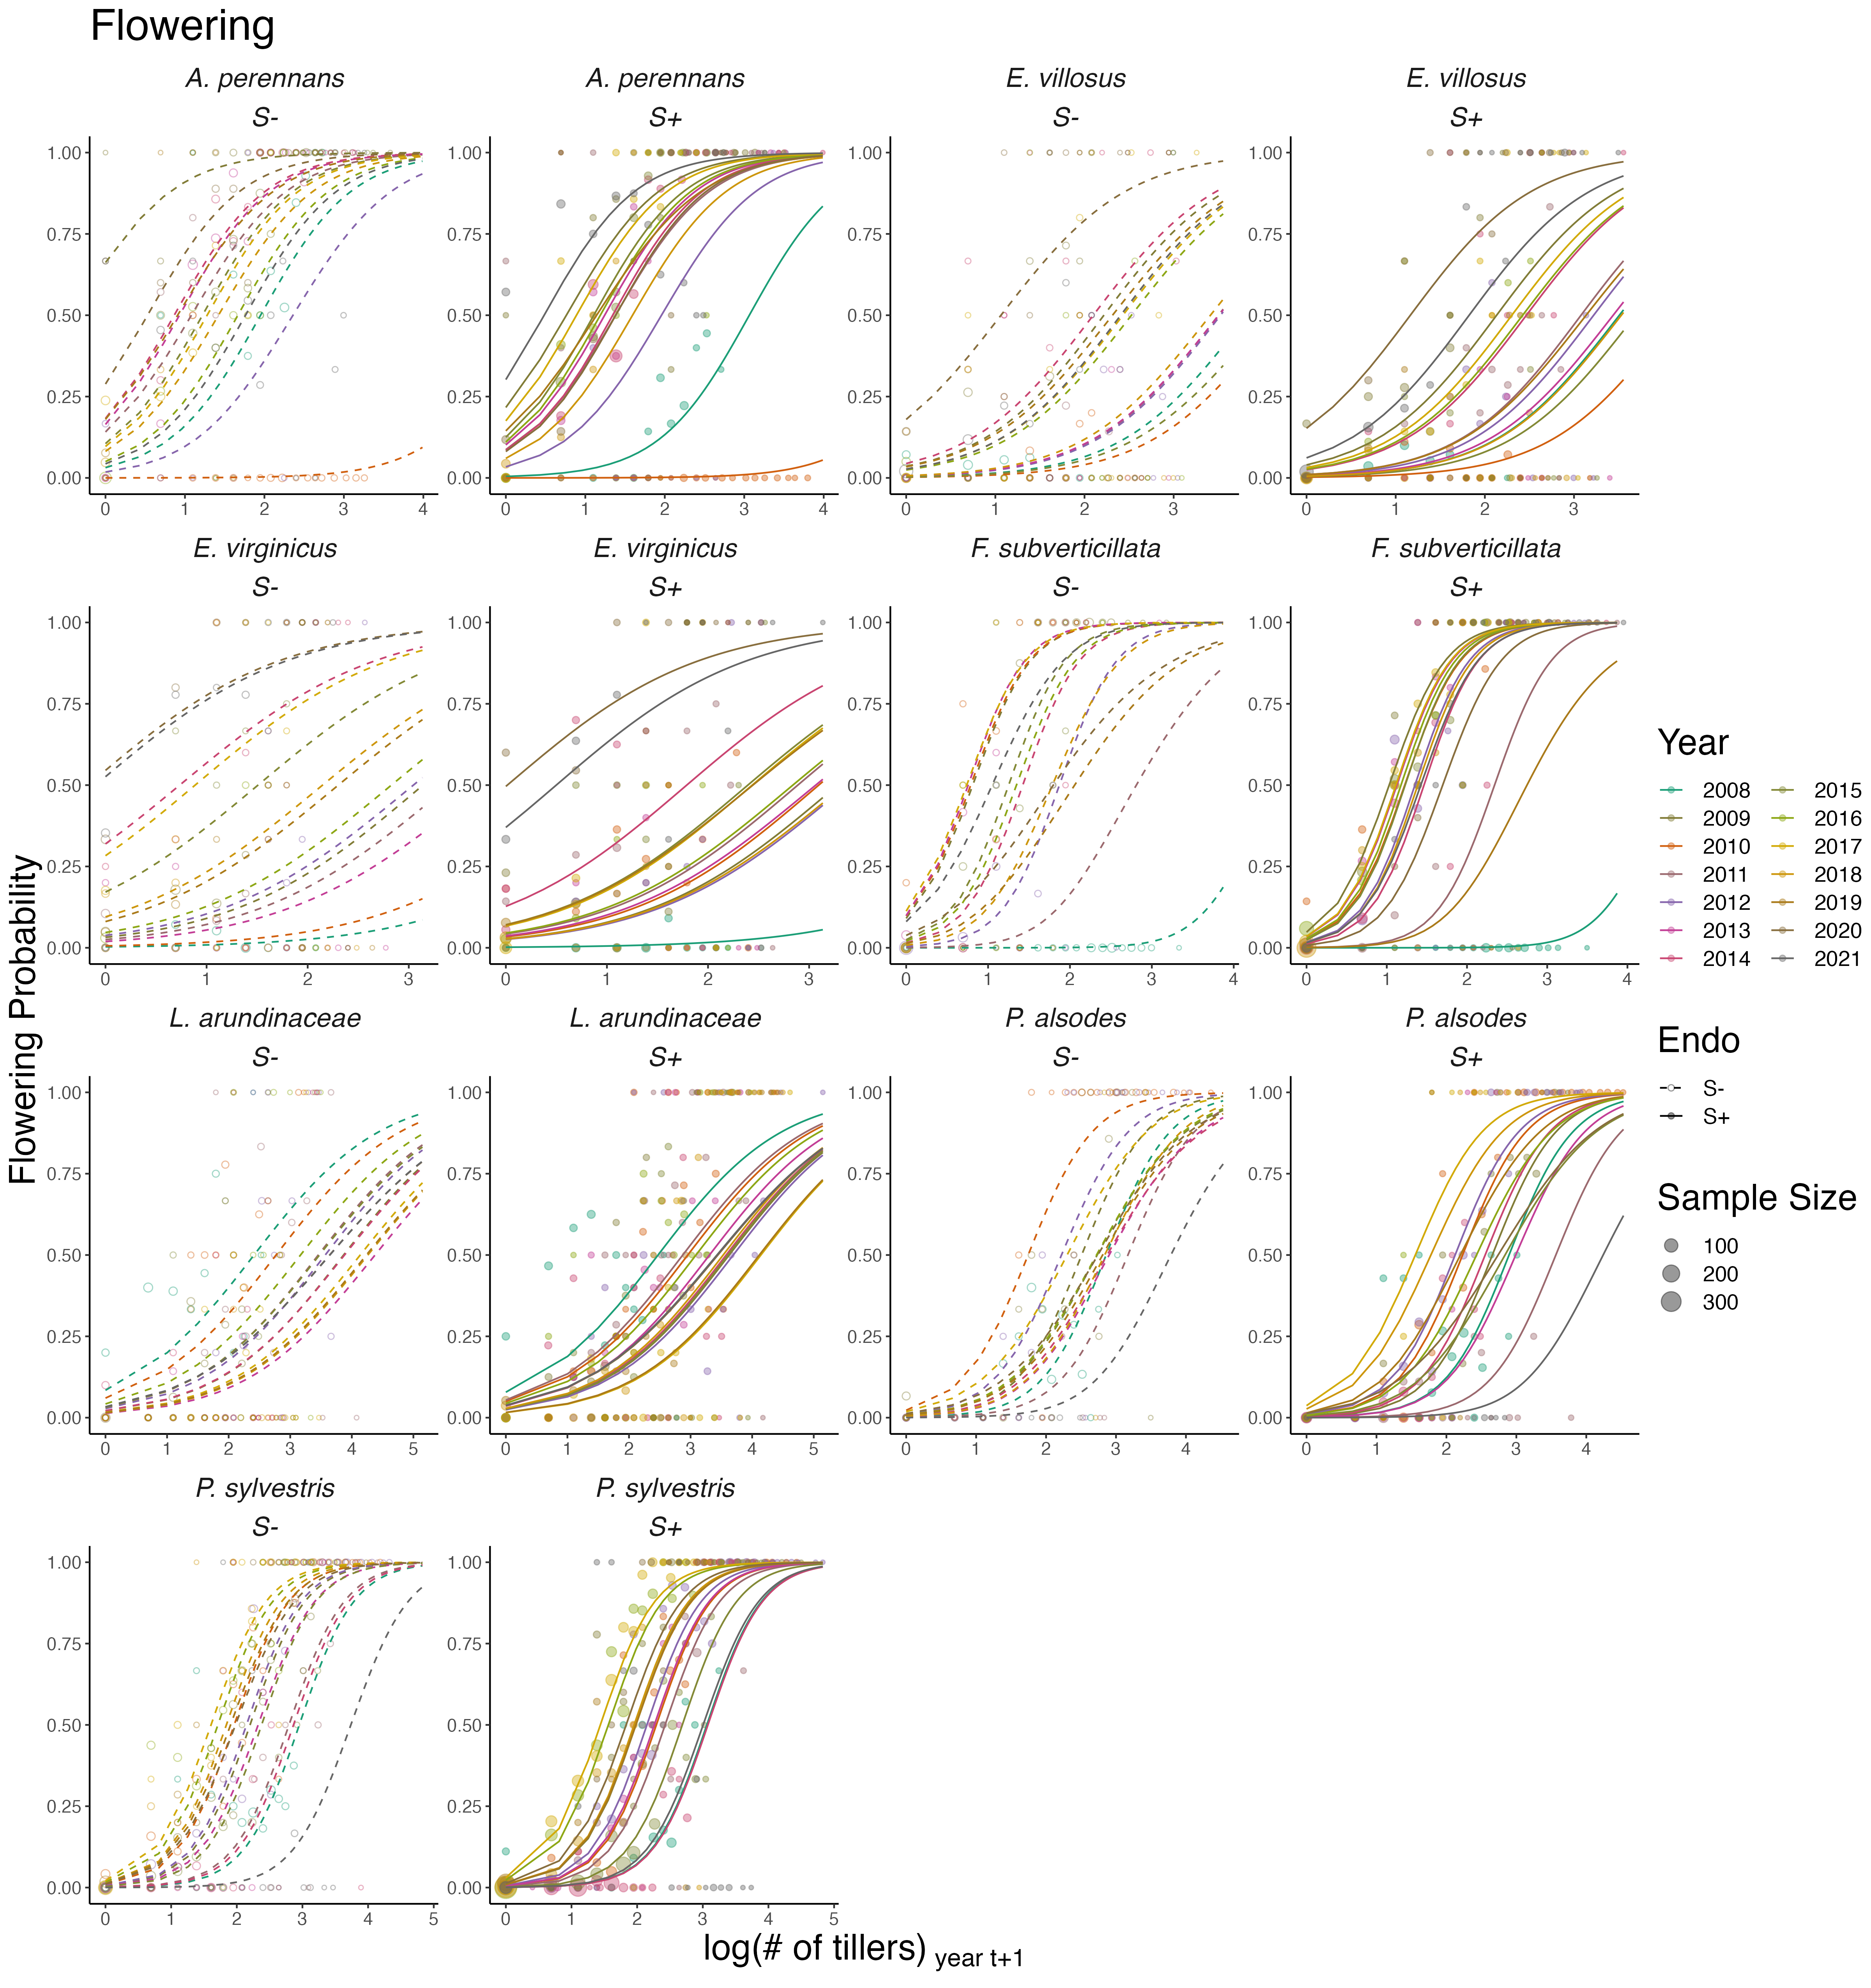
\includegraphics[width=.8\linewidth]{flw_yearplot.png}
\end{figure}
\noindent {\bf Fig. S8.} \textbf{Effect of endophyte symbiosis on yearly flowering} Fitted curves represent the size-specific annual flowering probability along with data binned by size shown as open circles with a dashed line for symbiont-free (S-) plants , while the solid line and filled circles represent symbiontic (S+) plants.
\begin{figure}[H]
	\centering
	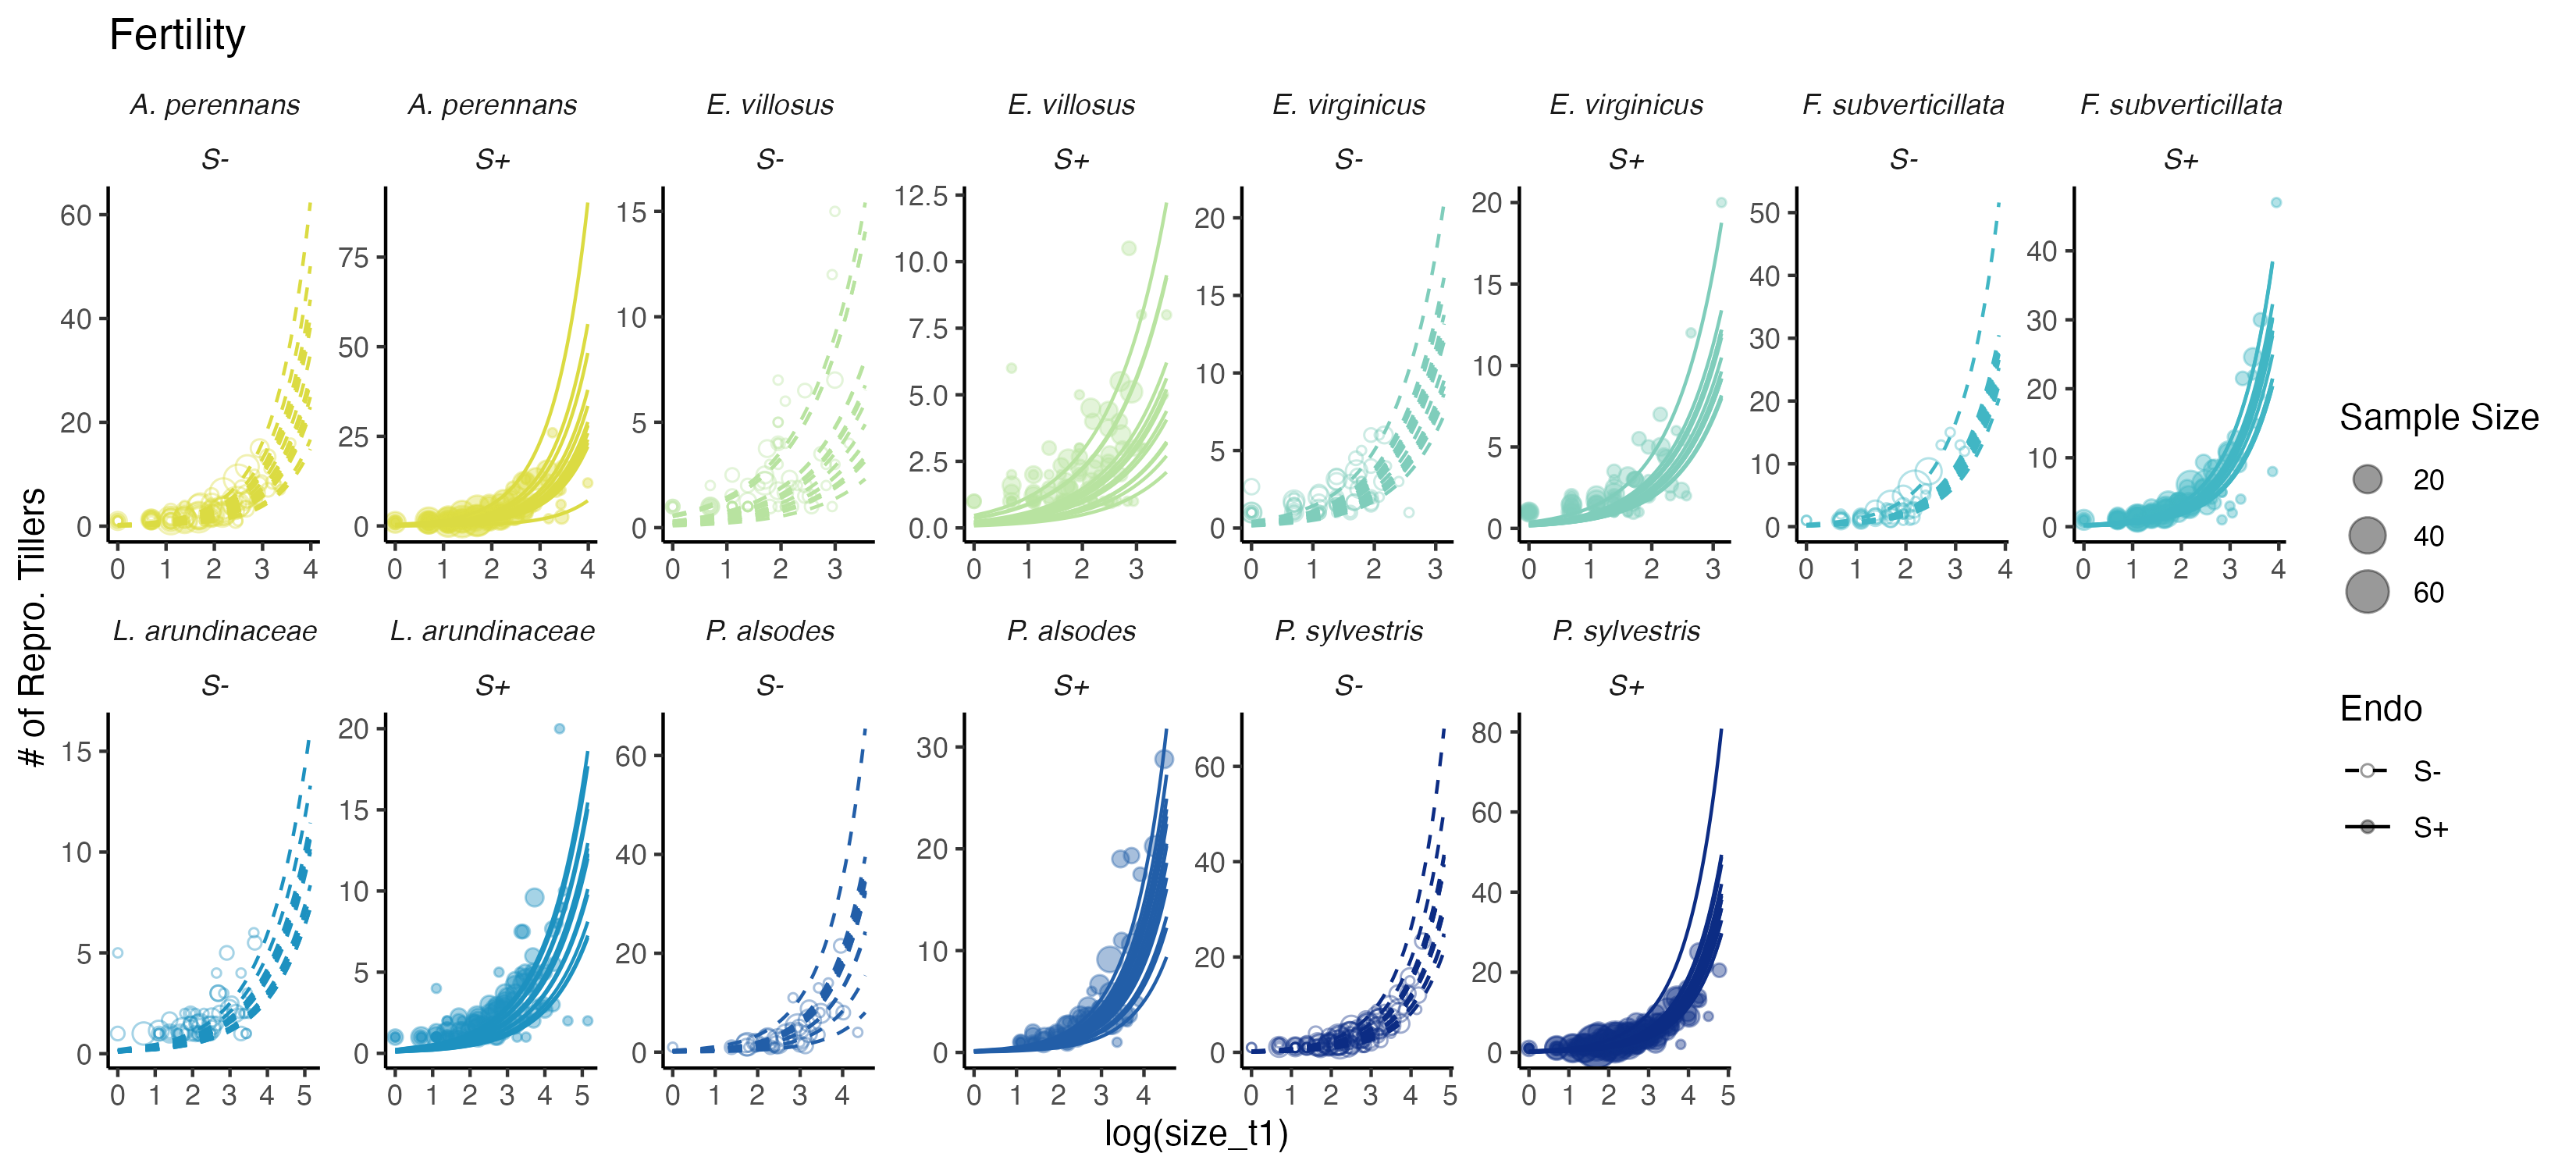
\includegraphics[width=.8\linewidth]{fert_yearplot.png}
\end{figure}
\noindent {\bf Fig. S9.} \textbf{Effect of endophyte symbiosis on yearly fertility.} Fitted curves represent the size-specific annual expected number of flowering tillers along with data binned by size shown as open circles with a dashed line for symbiont-free (S-) plants , while the solid line and filled circles represent symbiontic (S+) plants. 
\newpage
\begin{figure}[H]
	\centering
	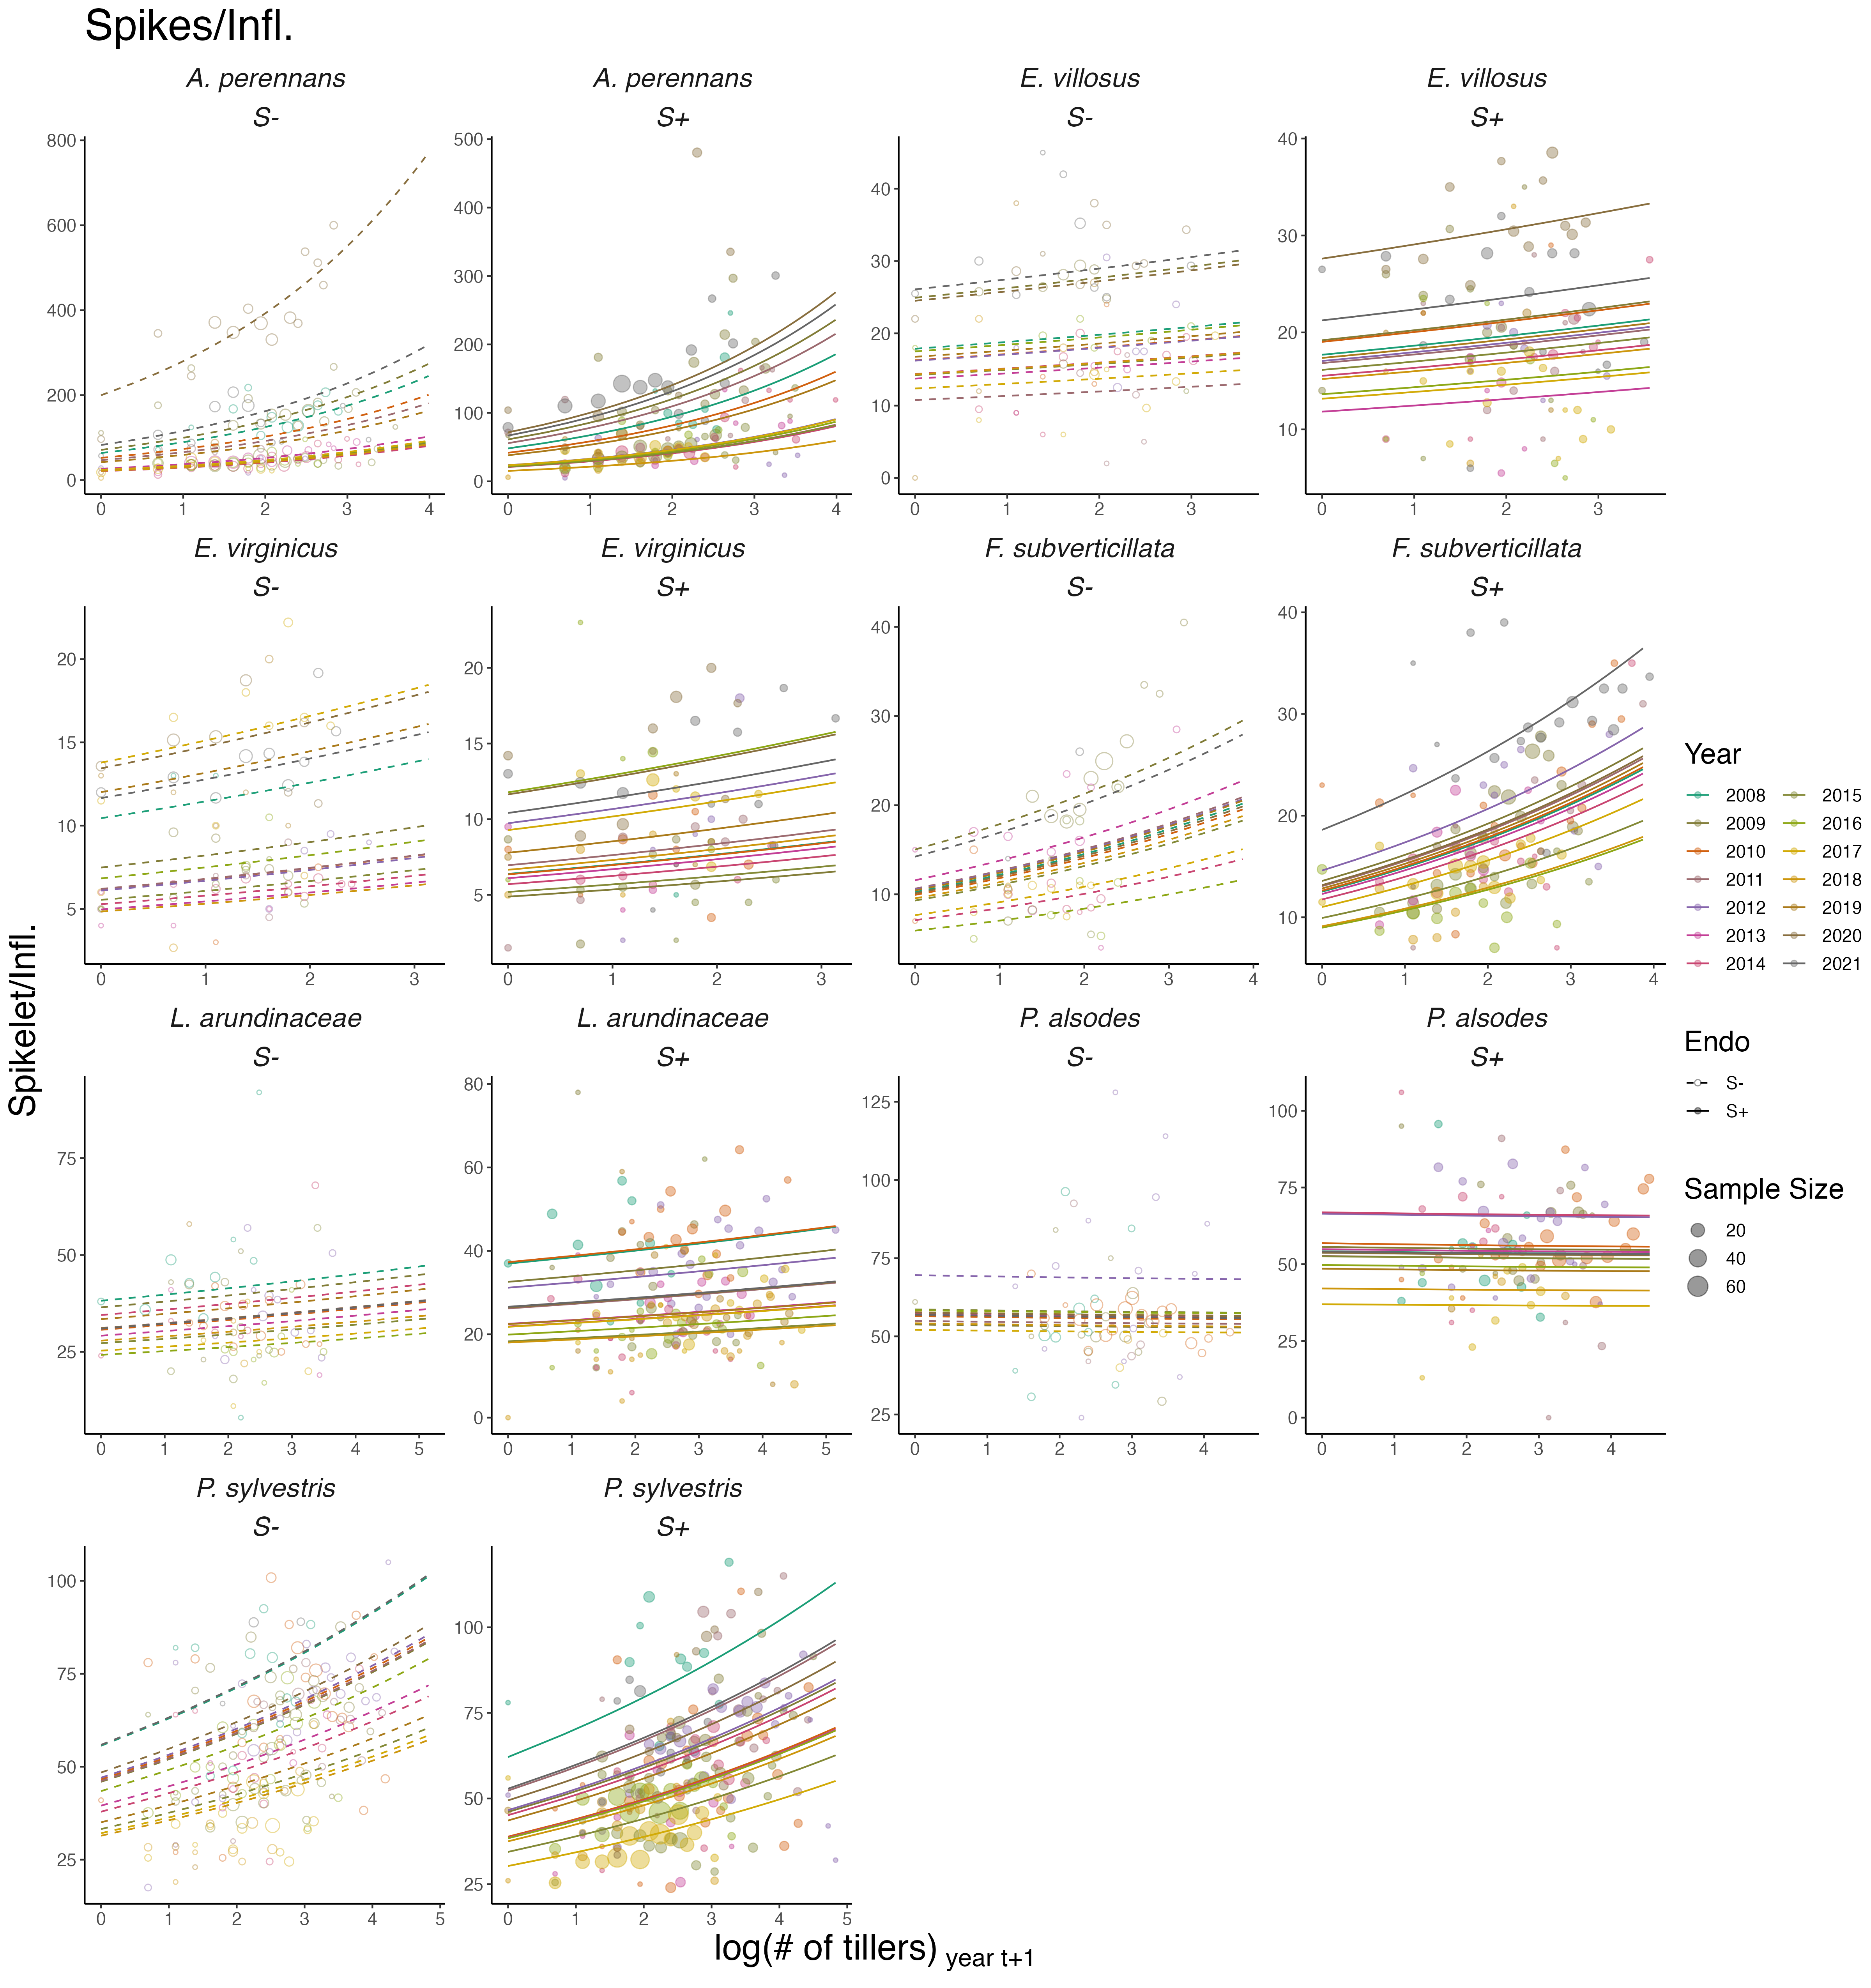
\includegraphics[width=.8\linewidth]{spike_yearplot.png}
\end{figure}
\noindent {\bf Fig. S10.} \textbf{Effect of endophyte symbiosis on yearly spikelet production.} Fitted curves represent the size-specific annual expected number of spikelets per inflorescence along with data binned by size shown as open circles with a dashed line for symbiont-free (S-) plants , while the solid line and filled circles represent symbiontic (S+) plants.
\newpage


\begin{figure}[H]
	\centering
	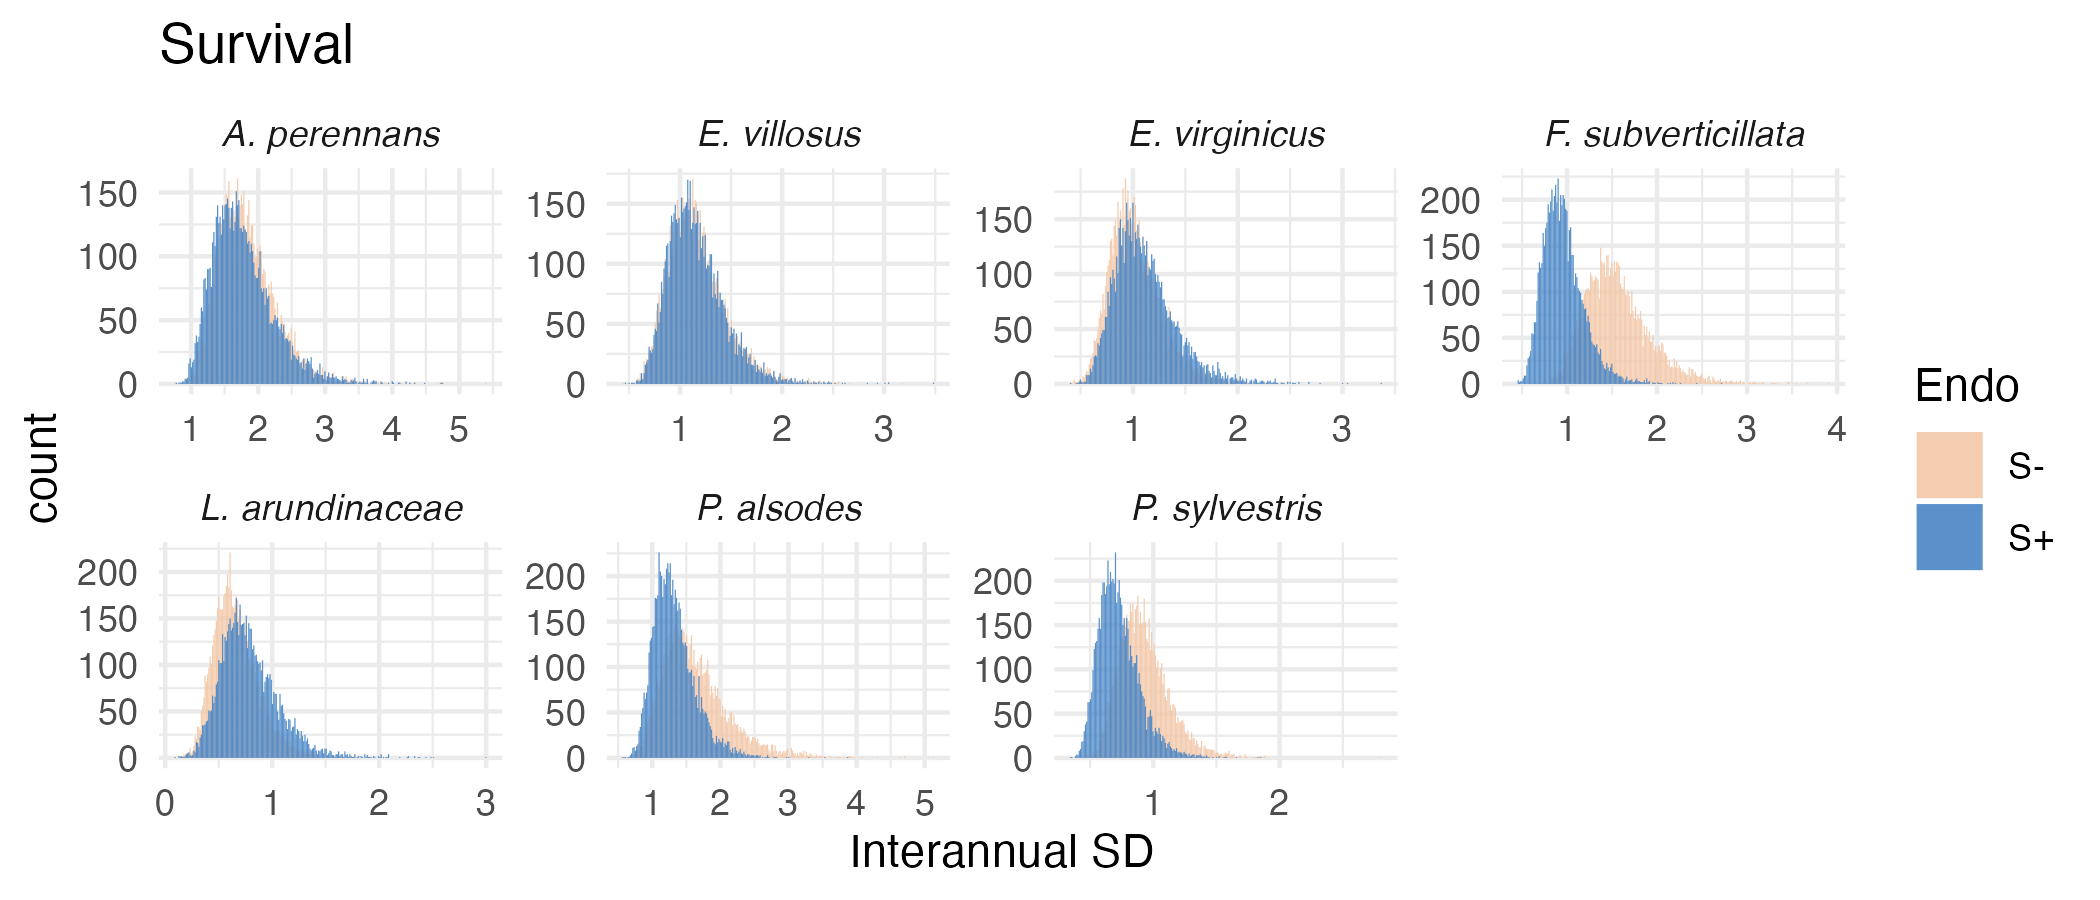
\includegraphics[width=.9\linewidth]{surv_sigmayear_hist.png}
\end{figure}
\noindent {\bf Fig. S11.} \textbf{Posterior distributions of the standard deviations of interannual year effects for survival.} Histograms include 7500 post-warmup MCMC samples for symbiotic (S+; blue) and symbiont-free (S-; tan) plants from fitted vital rate model.


\begin{figure}[H]
	\centering
	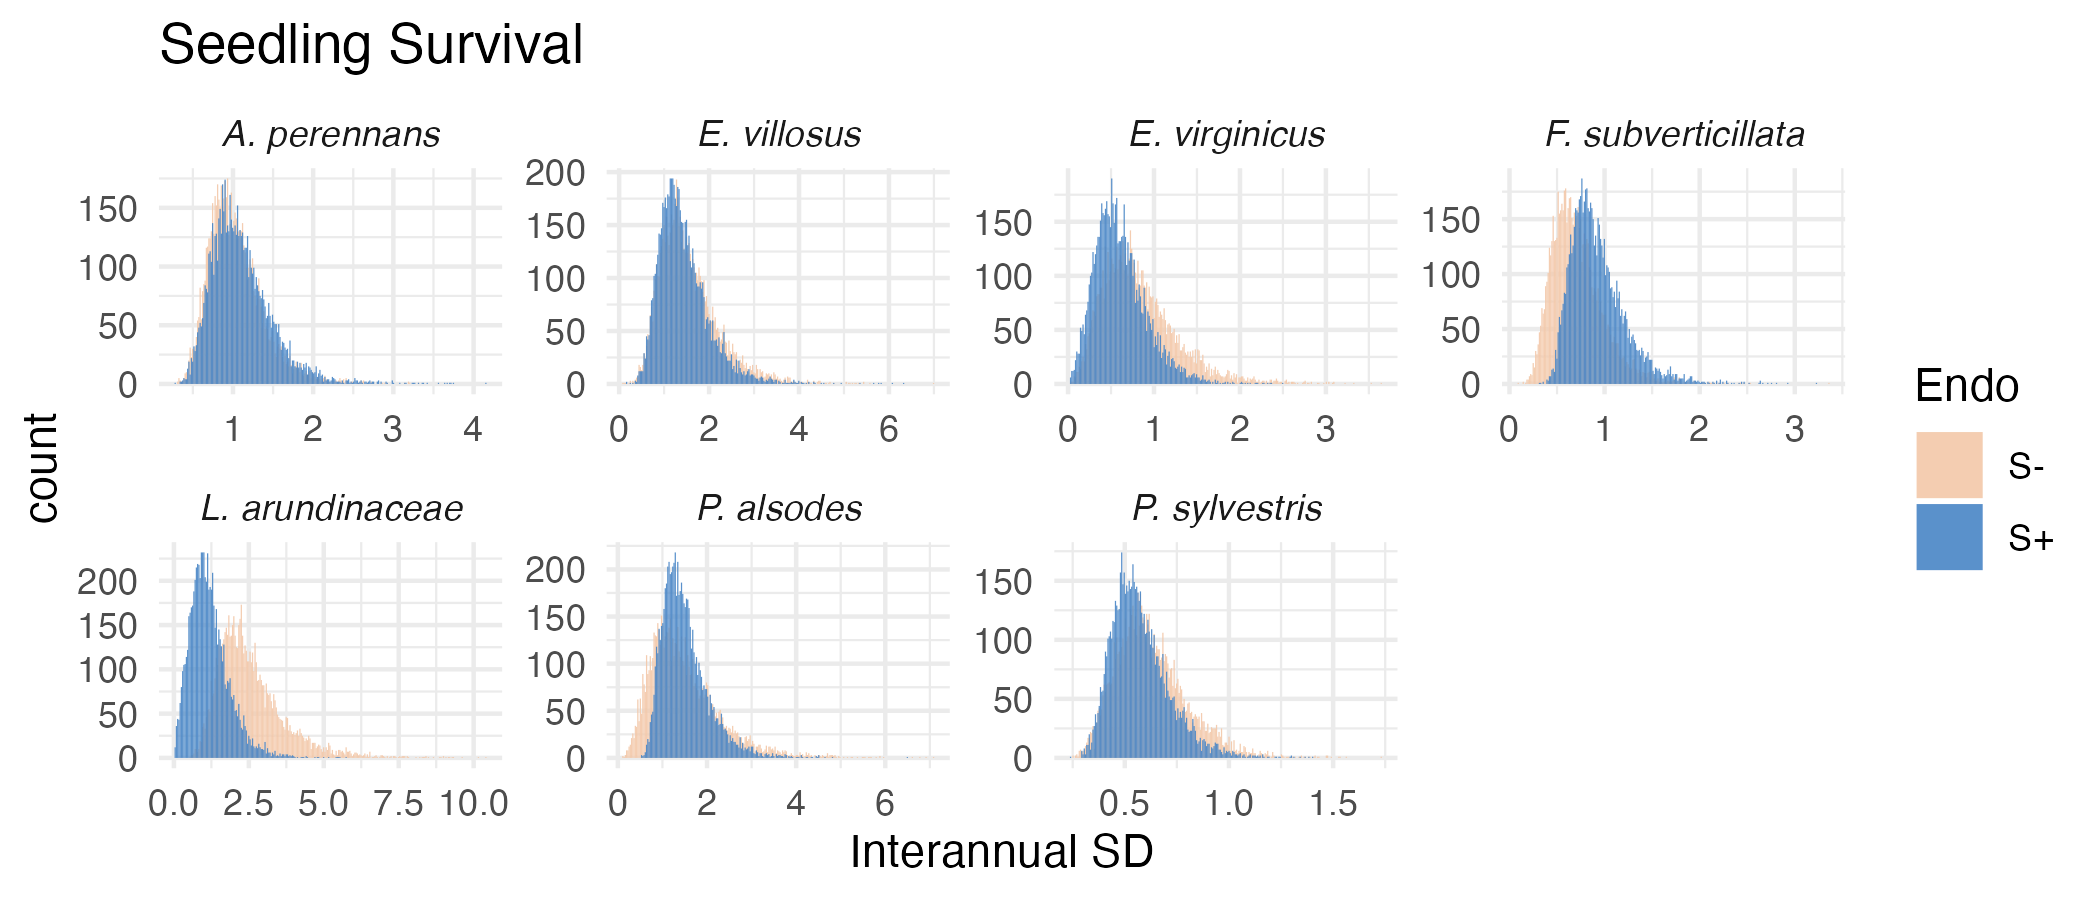
\includegraphics[width=.9\linewidth]{seedsurv_sigmayear_hist.png}
\end{figure}
\noindent {\bf Fig. S12.} \textbf{Posterior distributions of the standard deviations of interannual year effects for seedling survival.} Histograms include 7500 post-warmup MCMC samples for symbiotic (S+; blue) and symbiont-free (S-; tan) plants from fitted vital rate model.
\newpage

\begin{figure}[H]
	\centering
	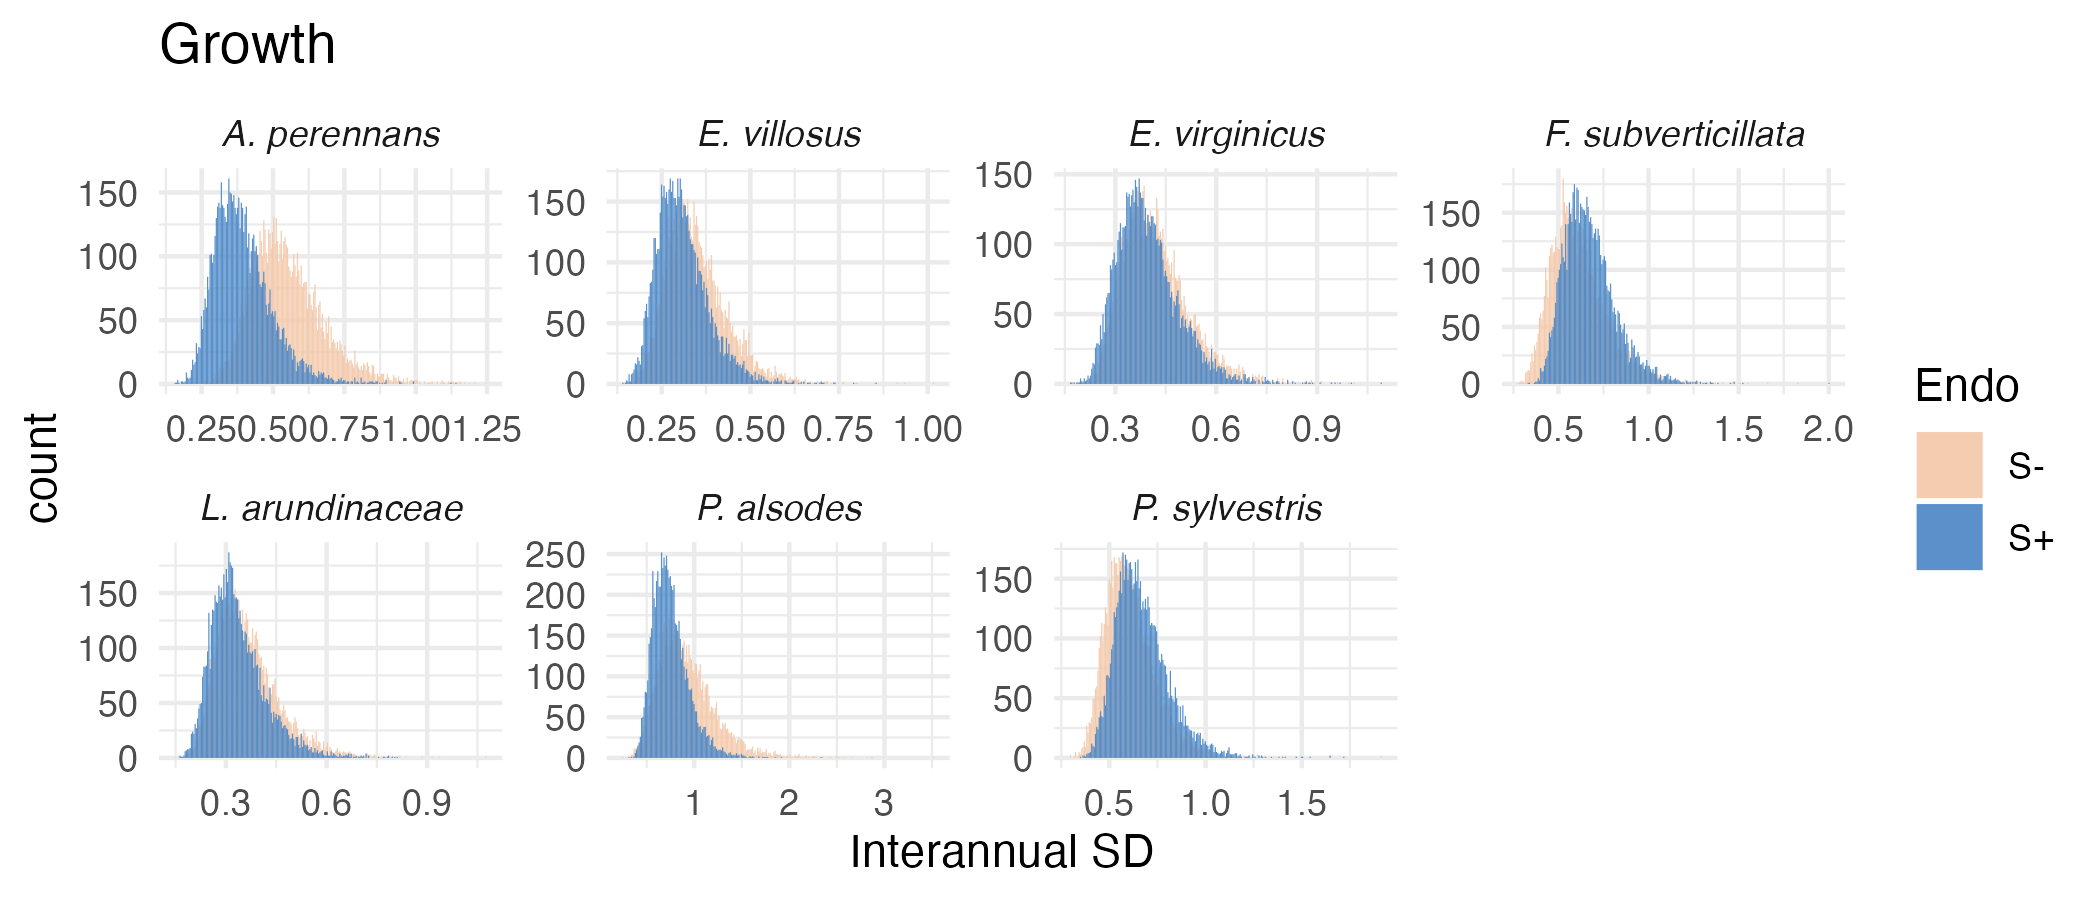
\includegraphics[width=.9\linewidth]{grow_sigmayear_hist.png}
\end{figure}
\noindent {\bf Fig. S13.} \textbf{Posterior distributions of the standard deviations of interannual year effects for growth.} Histograms include 7500 post-warmup MCMC samples for symbiotic (S+; blue) and symbiont-free (S-; tan) plants from fitted vital rate model.

\begin{figure}[H]
	\centering
	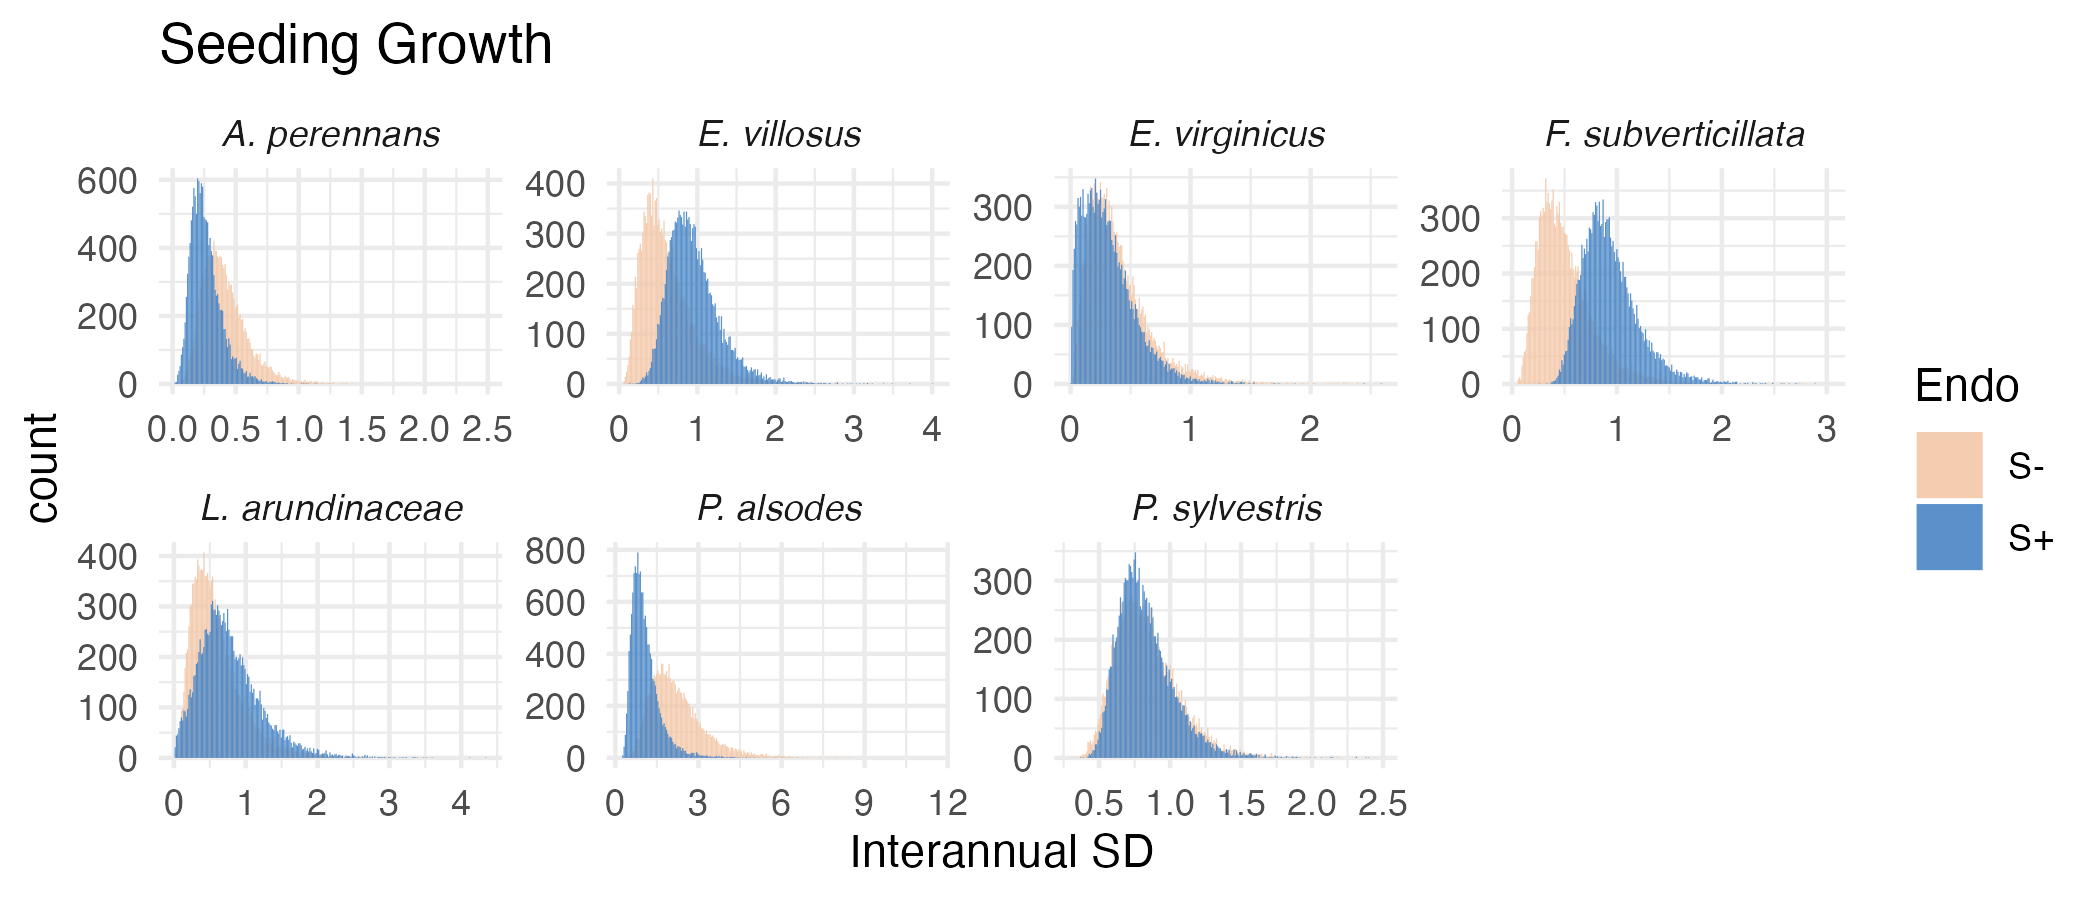
\includegraphics[width=.9\linewidth]{seedgrow_sigmayear_hist.png}
\end{figure}
\noindent {\bf Fig. S14.} \textbf{Posterior distributions of the standard deviations of interannual year effects for seedling growth.} Histograms include 7500 post-warmup MCMC samples for symbiotic (S+; blue) and symbiont-free (S-; tan) plants from fitted vital rate model.
\newpage

\begin{figure}[H]
	\centering
	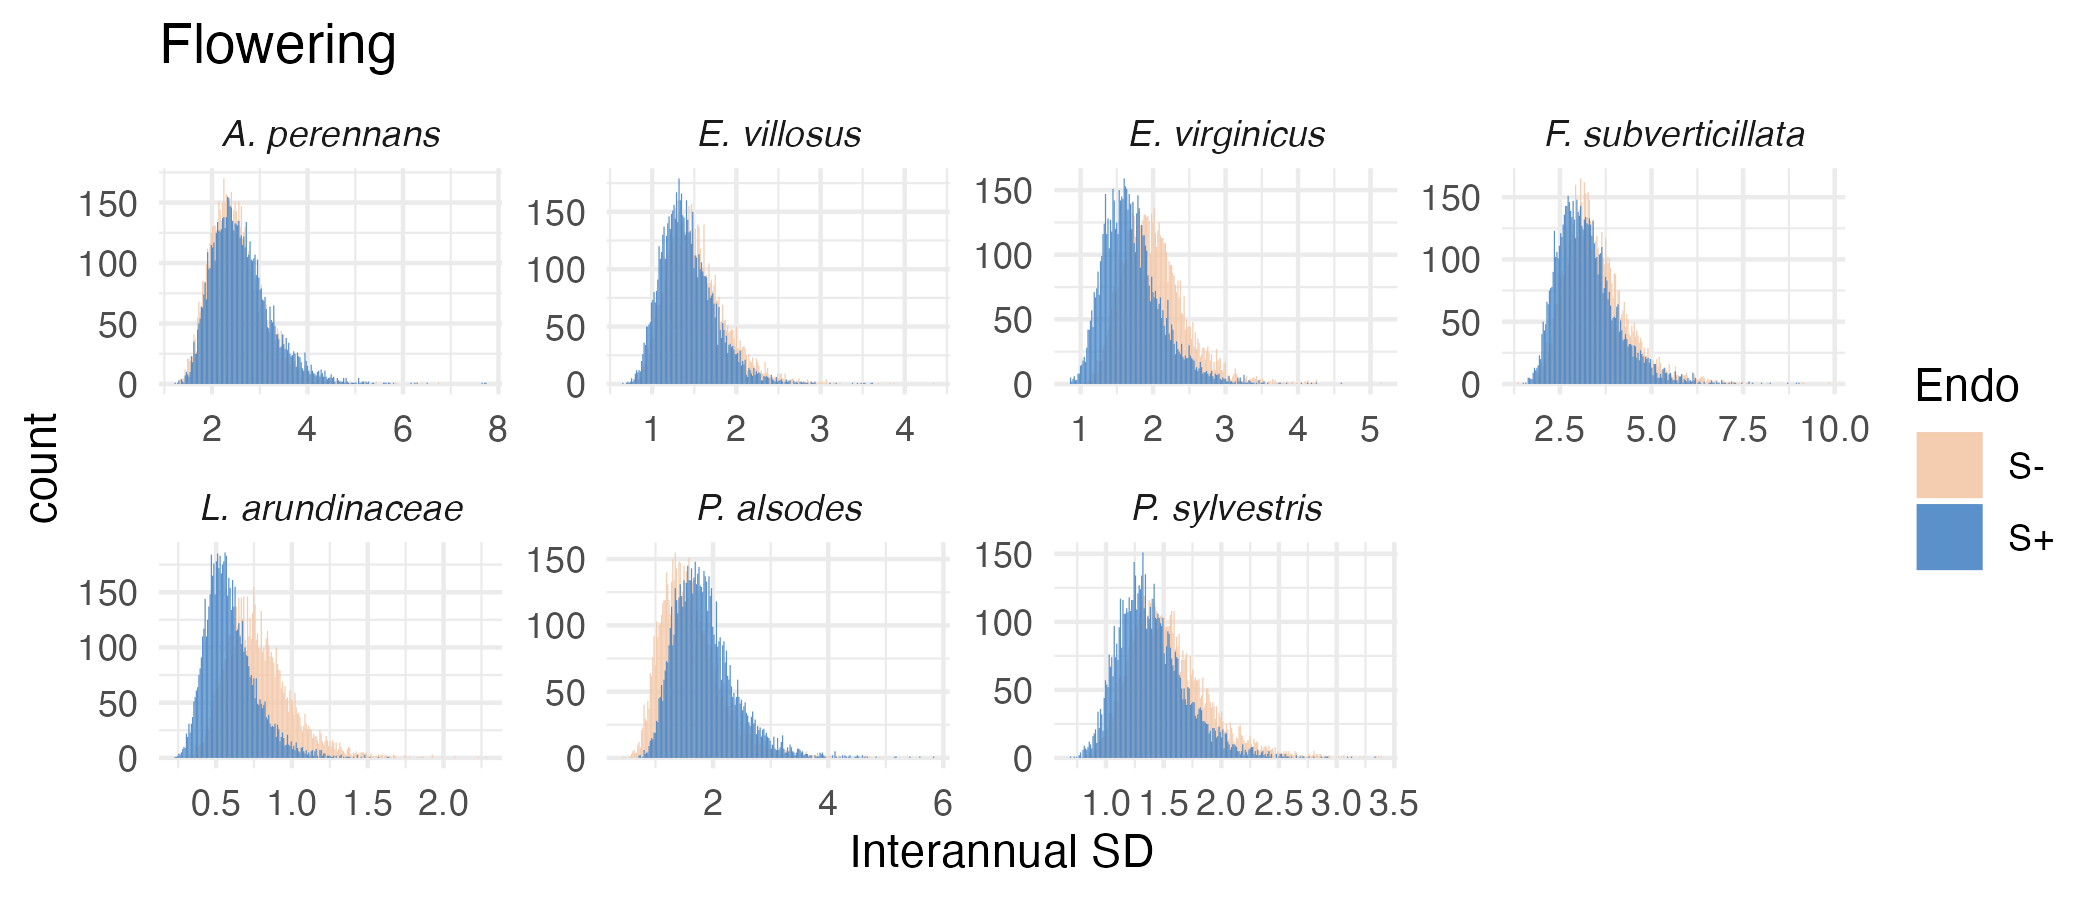
\includegraphics[width=.9\linewidth]{flow_sigmayear_hist.png}
\end{figure}
\noindent {\bf Fig. S15.} \textbf{Posterior distributions of the standard deviations of interannual year effects for flowering probability.} Histograms include 7500 post-warmup MCMC samples for symbiotic (S+; blue) and symbiont-free (S-; tan) plants from fitted vital rate model.


\begin{figure}[H]
	\centering
	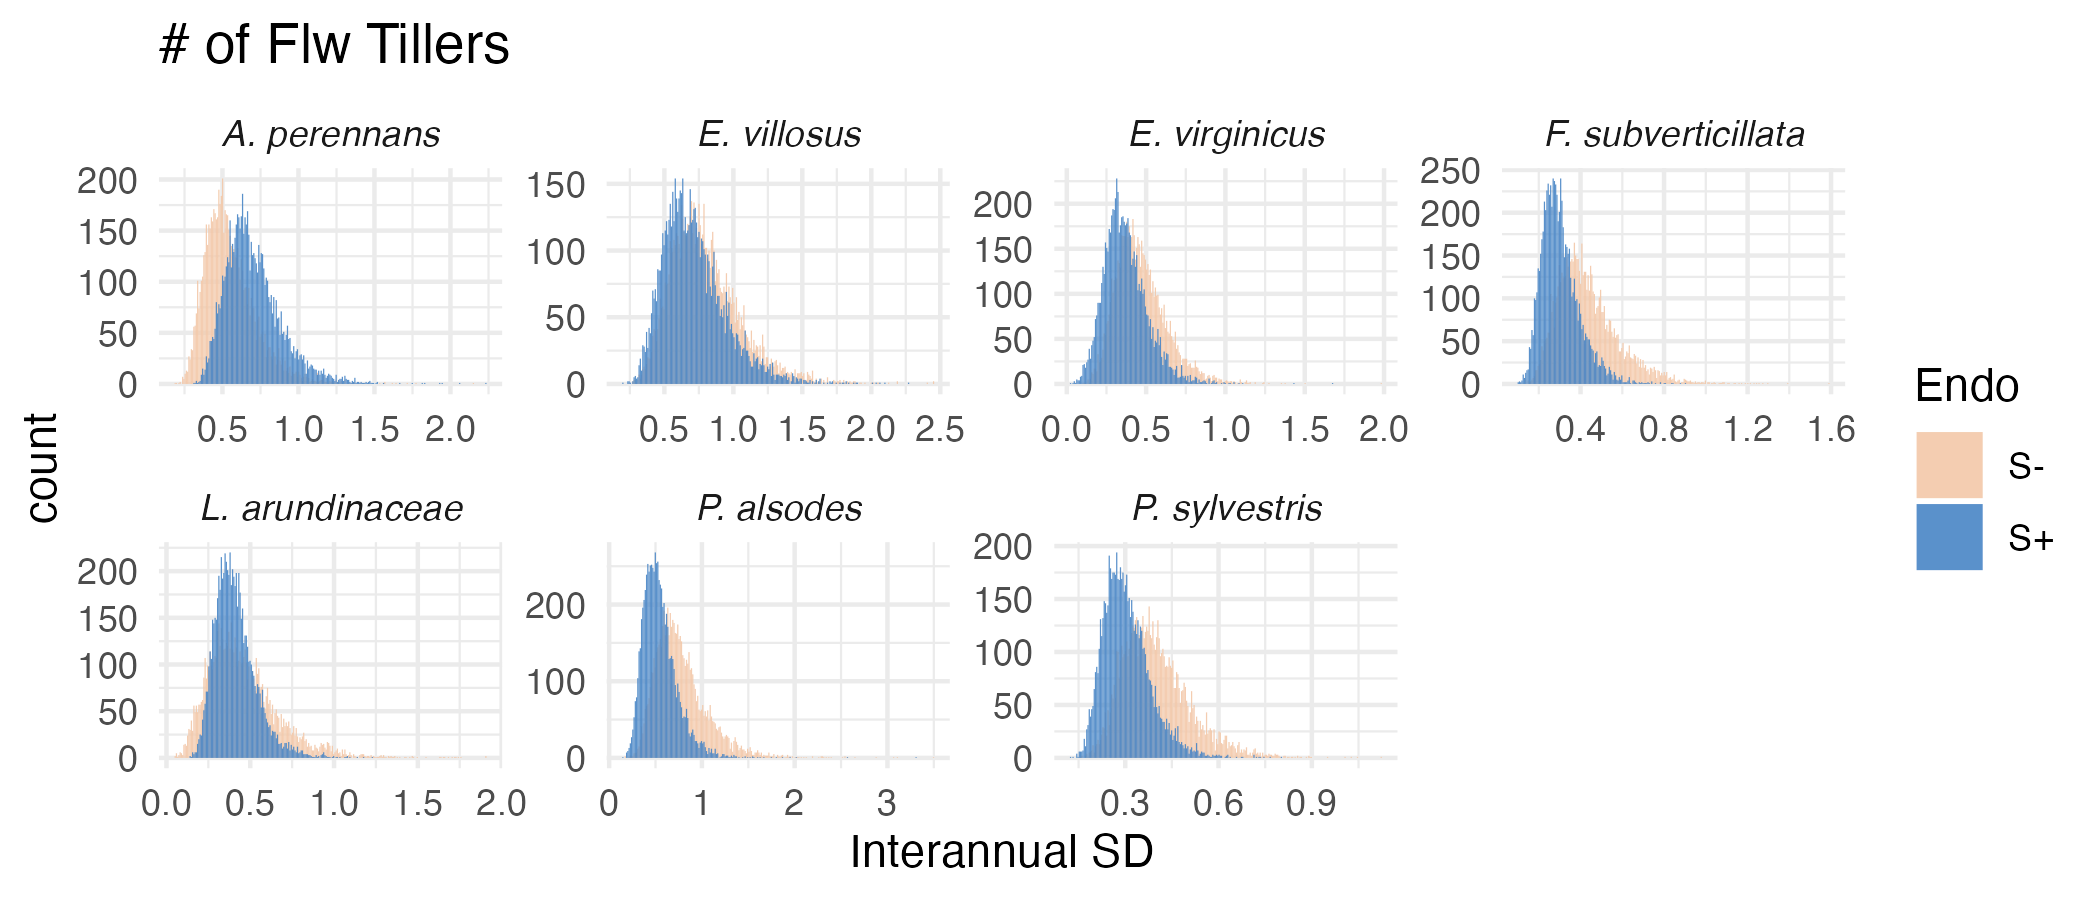
\includegraphics[width=.9\linewidth]{fert_sigmayear_hist.png}
\end{figure}
\noindent {\bf Fig. S16.} \textbf{Posterior distributions of the standard deviations of interannual year effects for fertility (no. of flowering tillers).} Histograms include 7500 post-warmup MCMC samples for symbiotic (S+; blue) and symbiont-free (S-; tan) plants from fitted vital rate model.
\newpage

\begin{figure}[H]
	\centering
	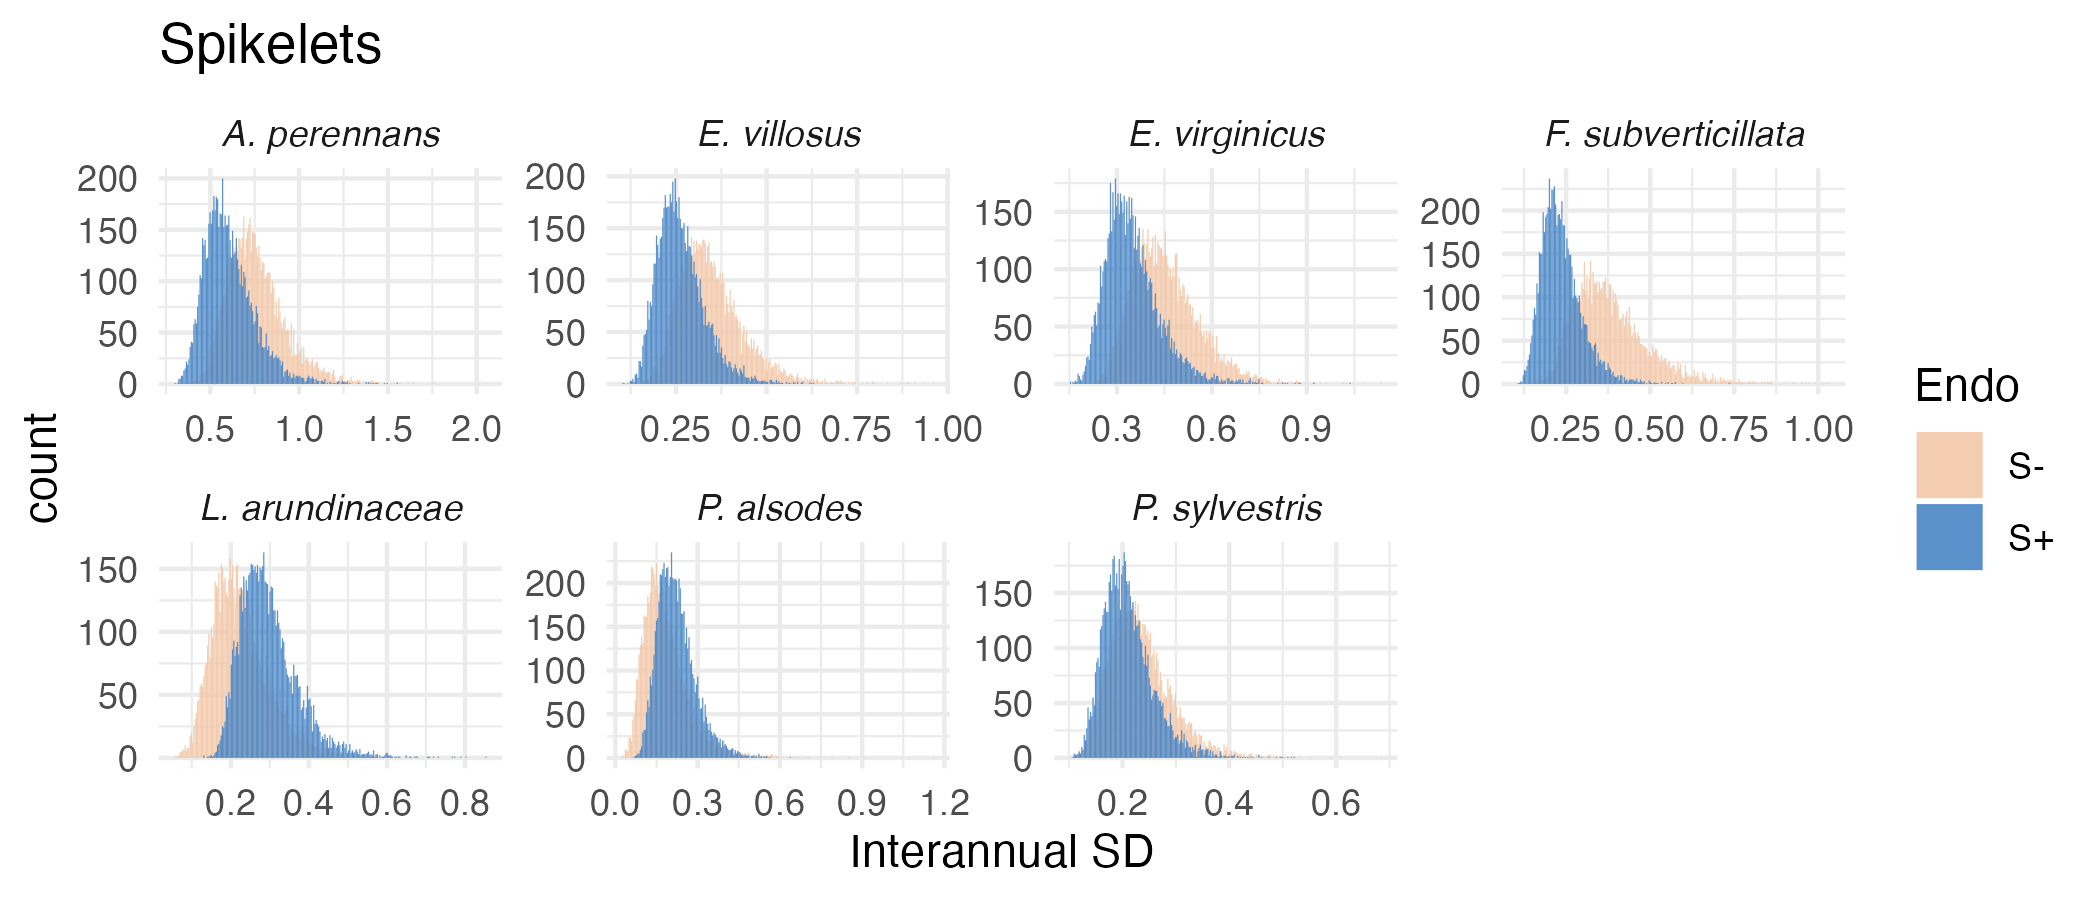
\includegraphics[width=.9\linewidth]{spike_sigmayear_hist.png}
\end{figure}
\noindent {\bf Fig. S17.} \textbf{Posterior distributions of the standard deviations of interannual year effects for spikelets per inflorescence.} Histograms include 7500 post-warmup MCMC samples for symbiotic (S+; blue) and symbiont-free (S-; tan) plants from fitted vital rate model.


\begin{figure}[H]
	\centering
	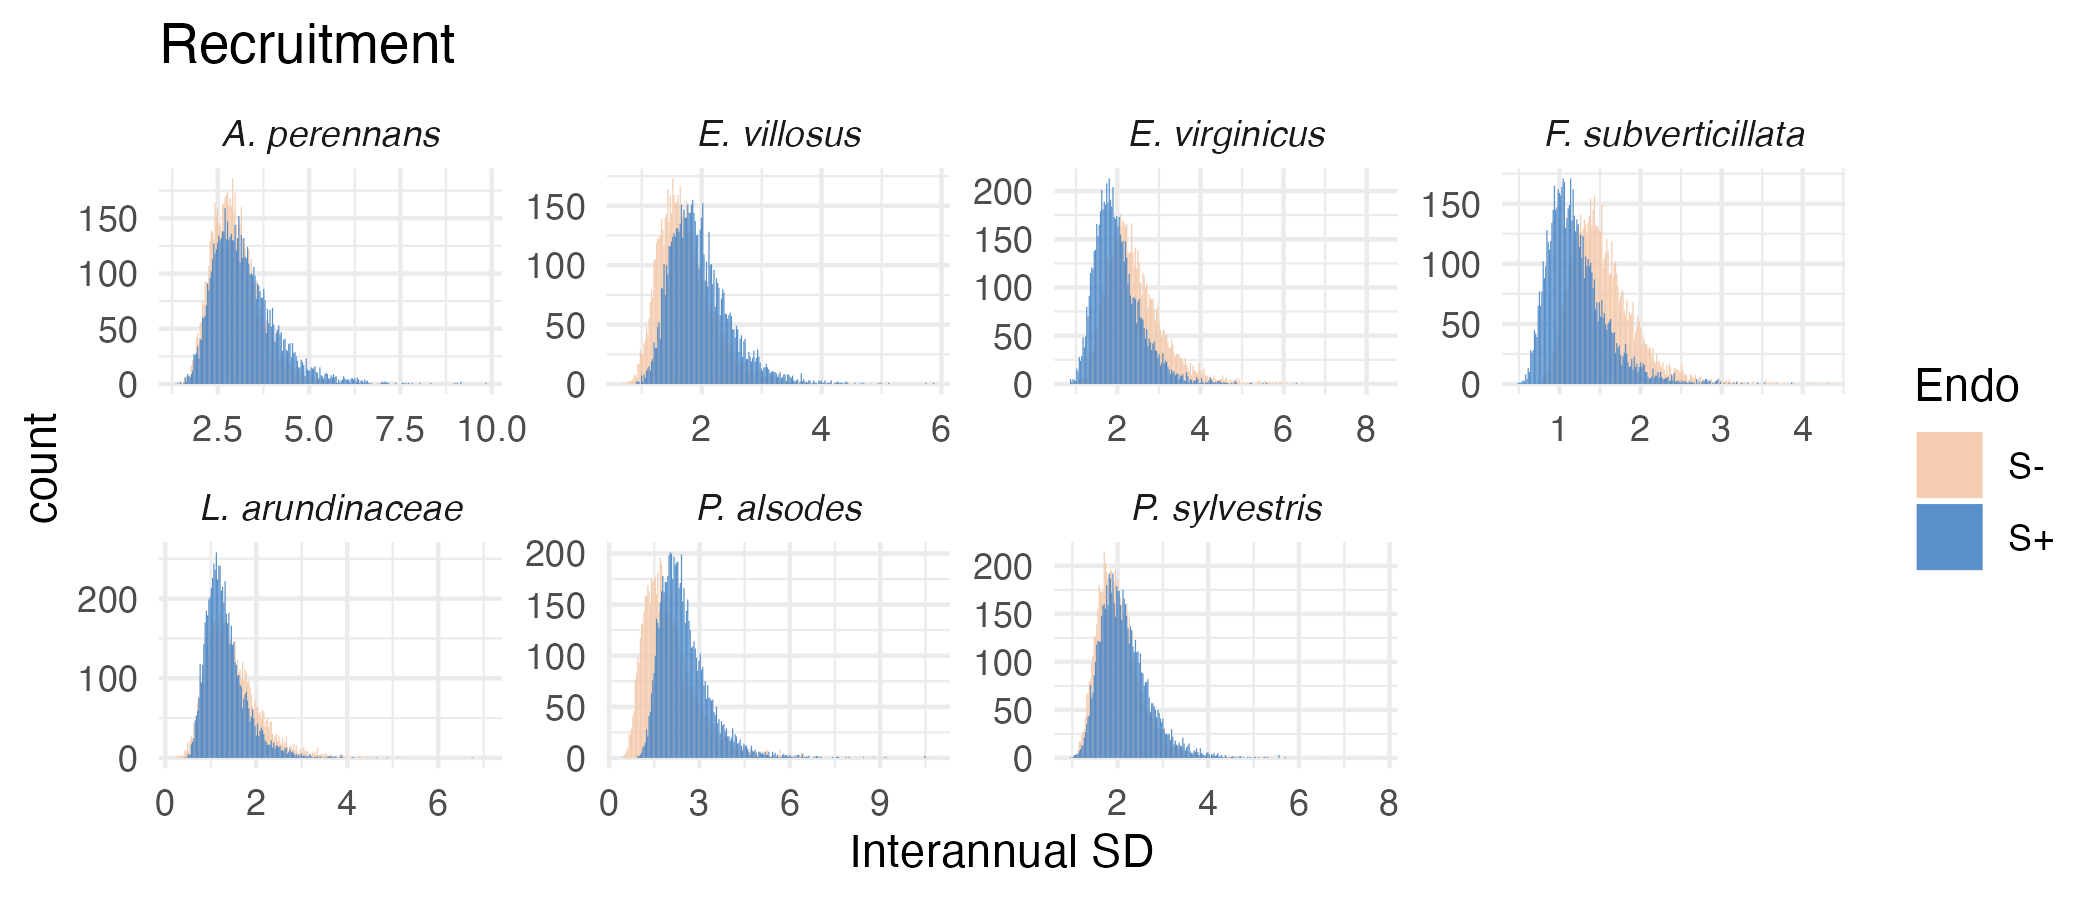
\includegraphics[width=.9\linewidth]{recruit_sigmayear_hist.png}
\end{figure}
\noindent {\bf Fig. S18.} \textbf{Posterior distributions of the standard deviations of interannual year effects for recruitment.} Histograms include 7500 post-warmup MCMC samples for symbiotic (S+; blue) and symbiont-free (S-; tan) plants from fitted vital rate model.

\newpage



\begin{figure}
	\centering
	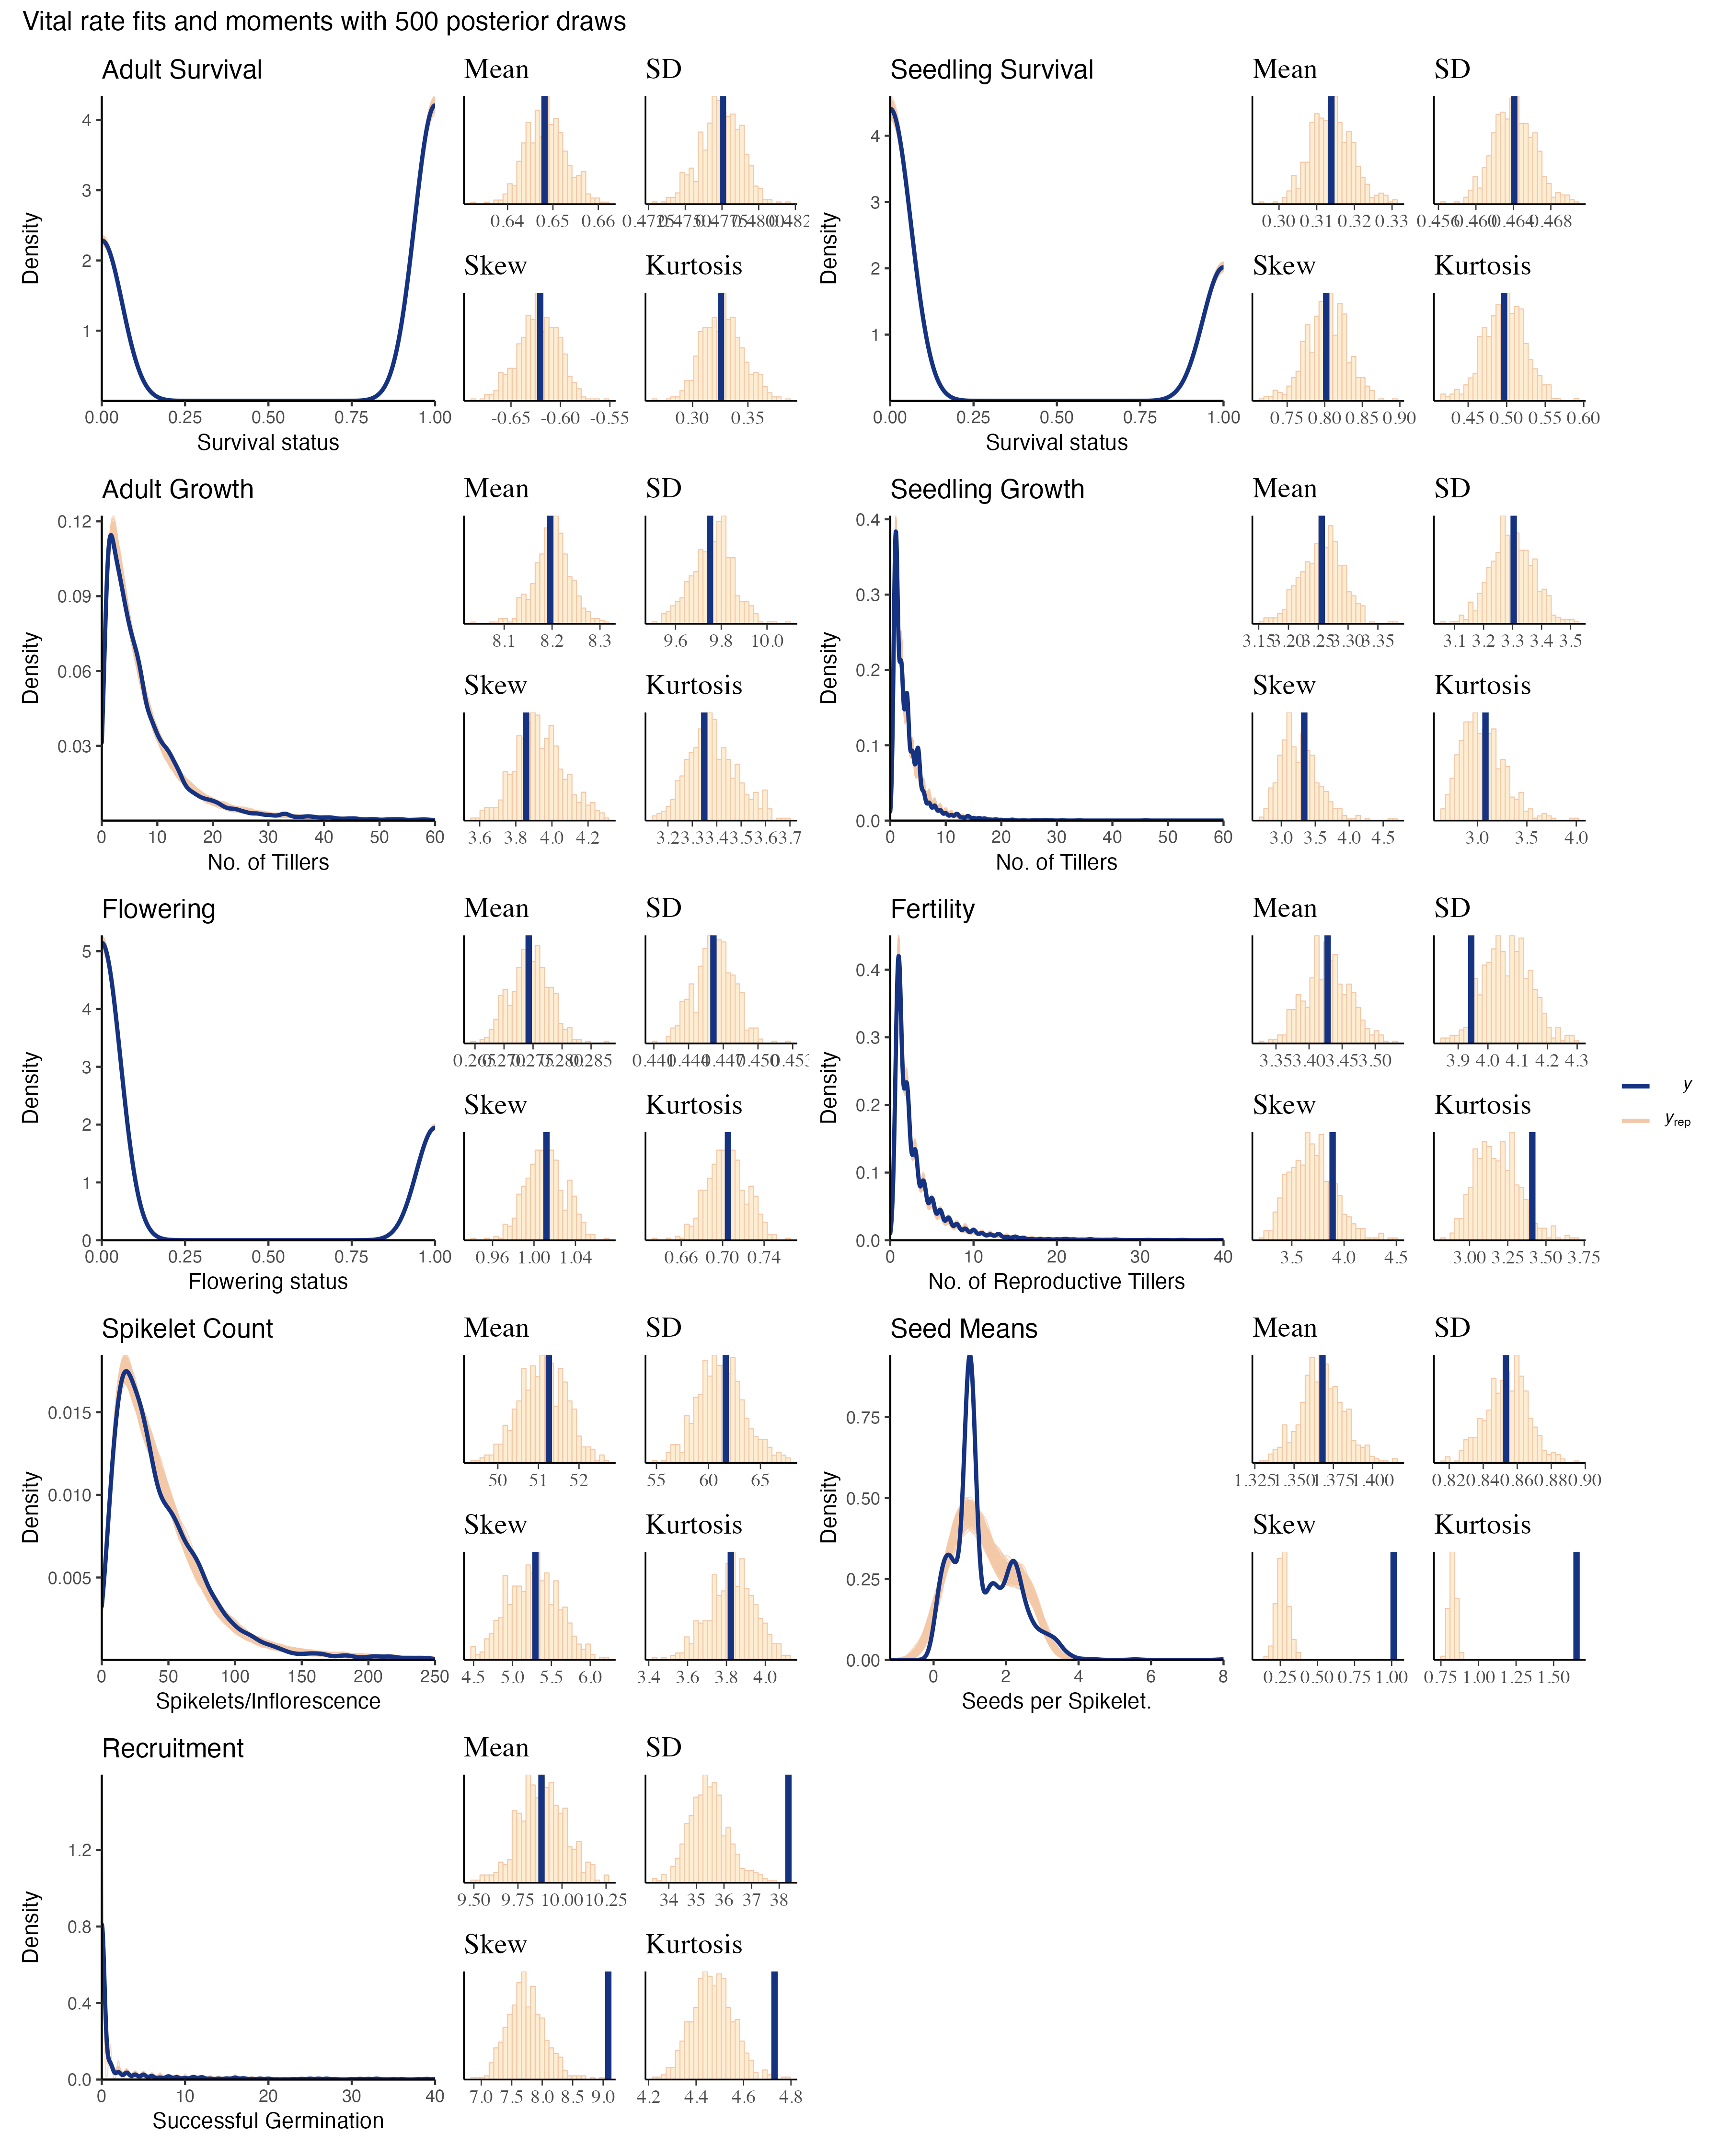
\includegraphics[width=.7\linewidth]{fitsandmoments_plot.png}
\end{figure}
\noindent {\bf Fig. S19.} \textbf{Consistency between real data and simulated values indicates that fitted models describe the data well.} Graphs show posterior predictive check for statistical models of demographic vital rates. Lines show density distributions of observed data (blue line) compared to data simulated from fitted models (tan lines) generated from 500 draws from posterior distributions of model parameters. 
\newpage

\begin{figure}
	\centering
	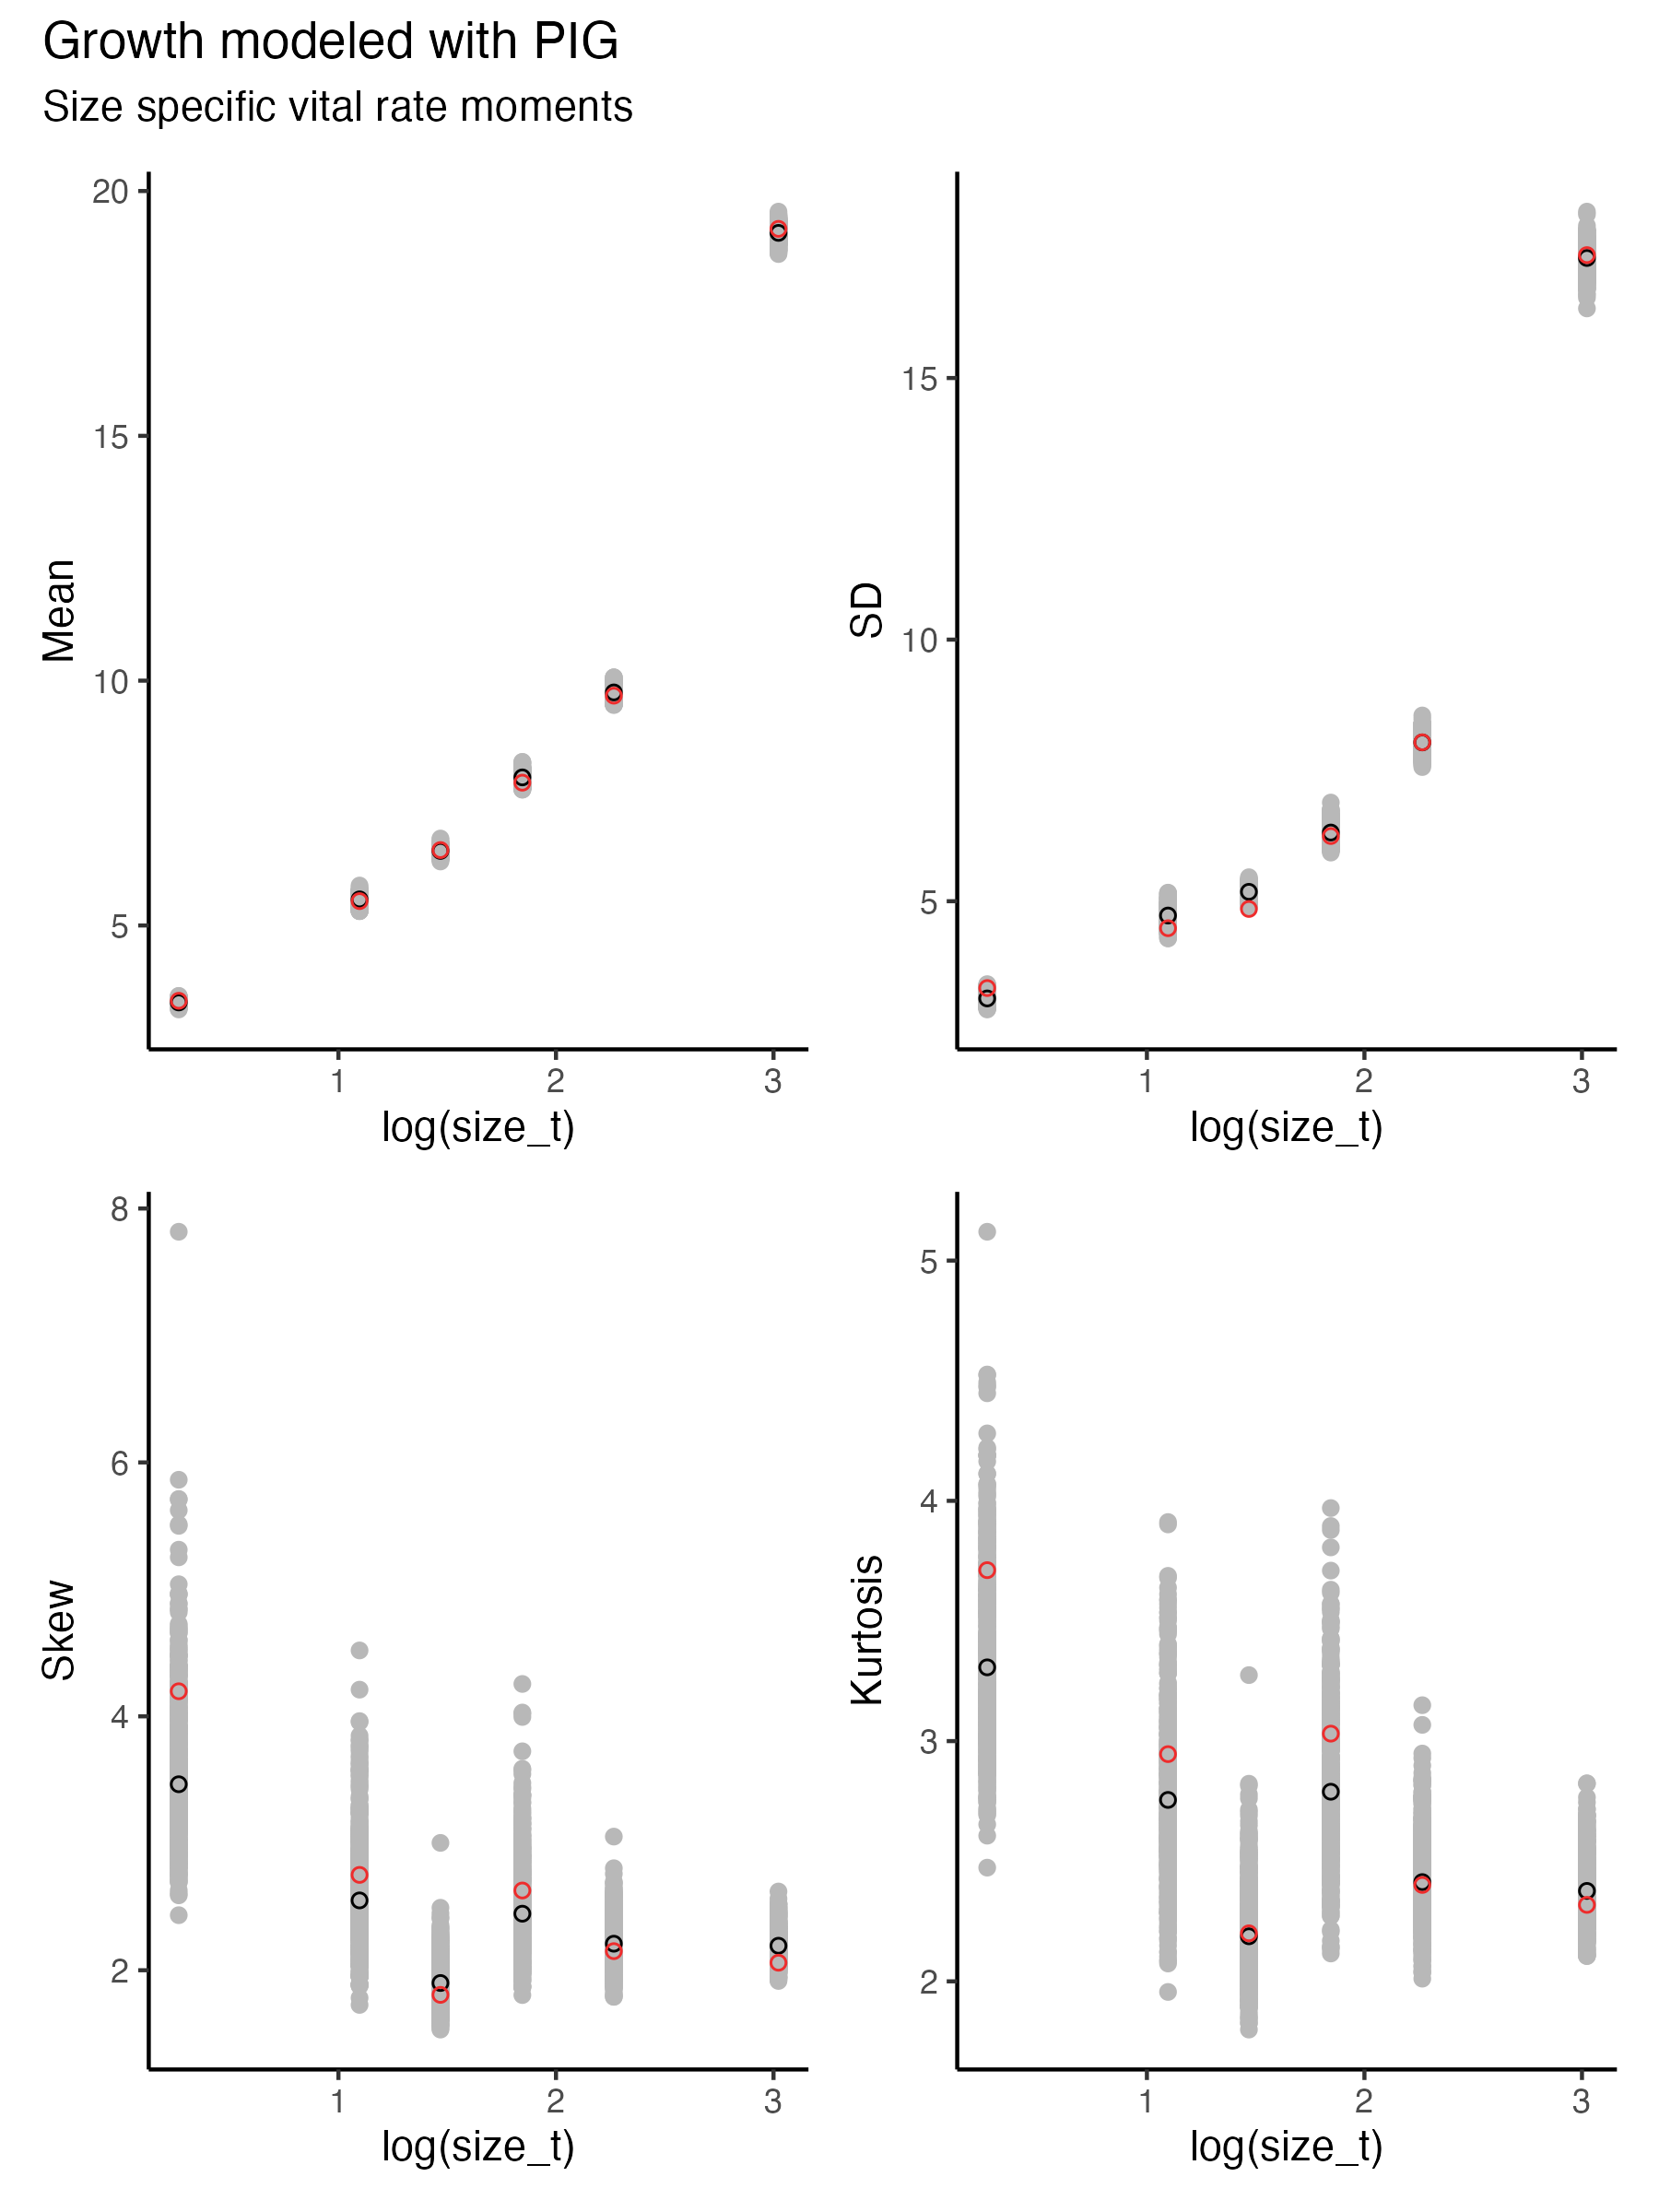
\includegraphics[width=.6\linewidth]{size_ppc_plot.png}
\end{figure}
\noindent {\bf Fig. S20.} \textbf{Consistency between real data and fitted values across sizes indicates that the growth model is accurately capturing size dependence} Graphs of posterior predictive check for mean and higher moments of the growth model across size. Points show the value of statistical moments binned across size for the observed data (red circles) compared to the simulated datasets (grey circles) and the median of the simulated values (black circles) generated from 500 posterior draws from the fitted model. 
\newpage

\begin{figure}
	\centering
	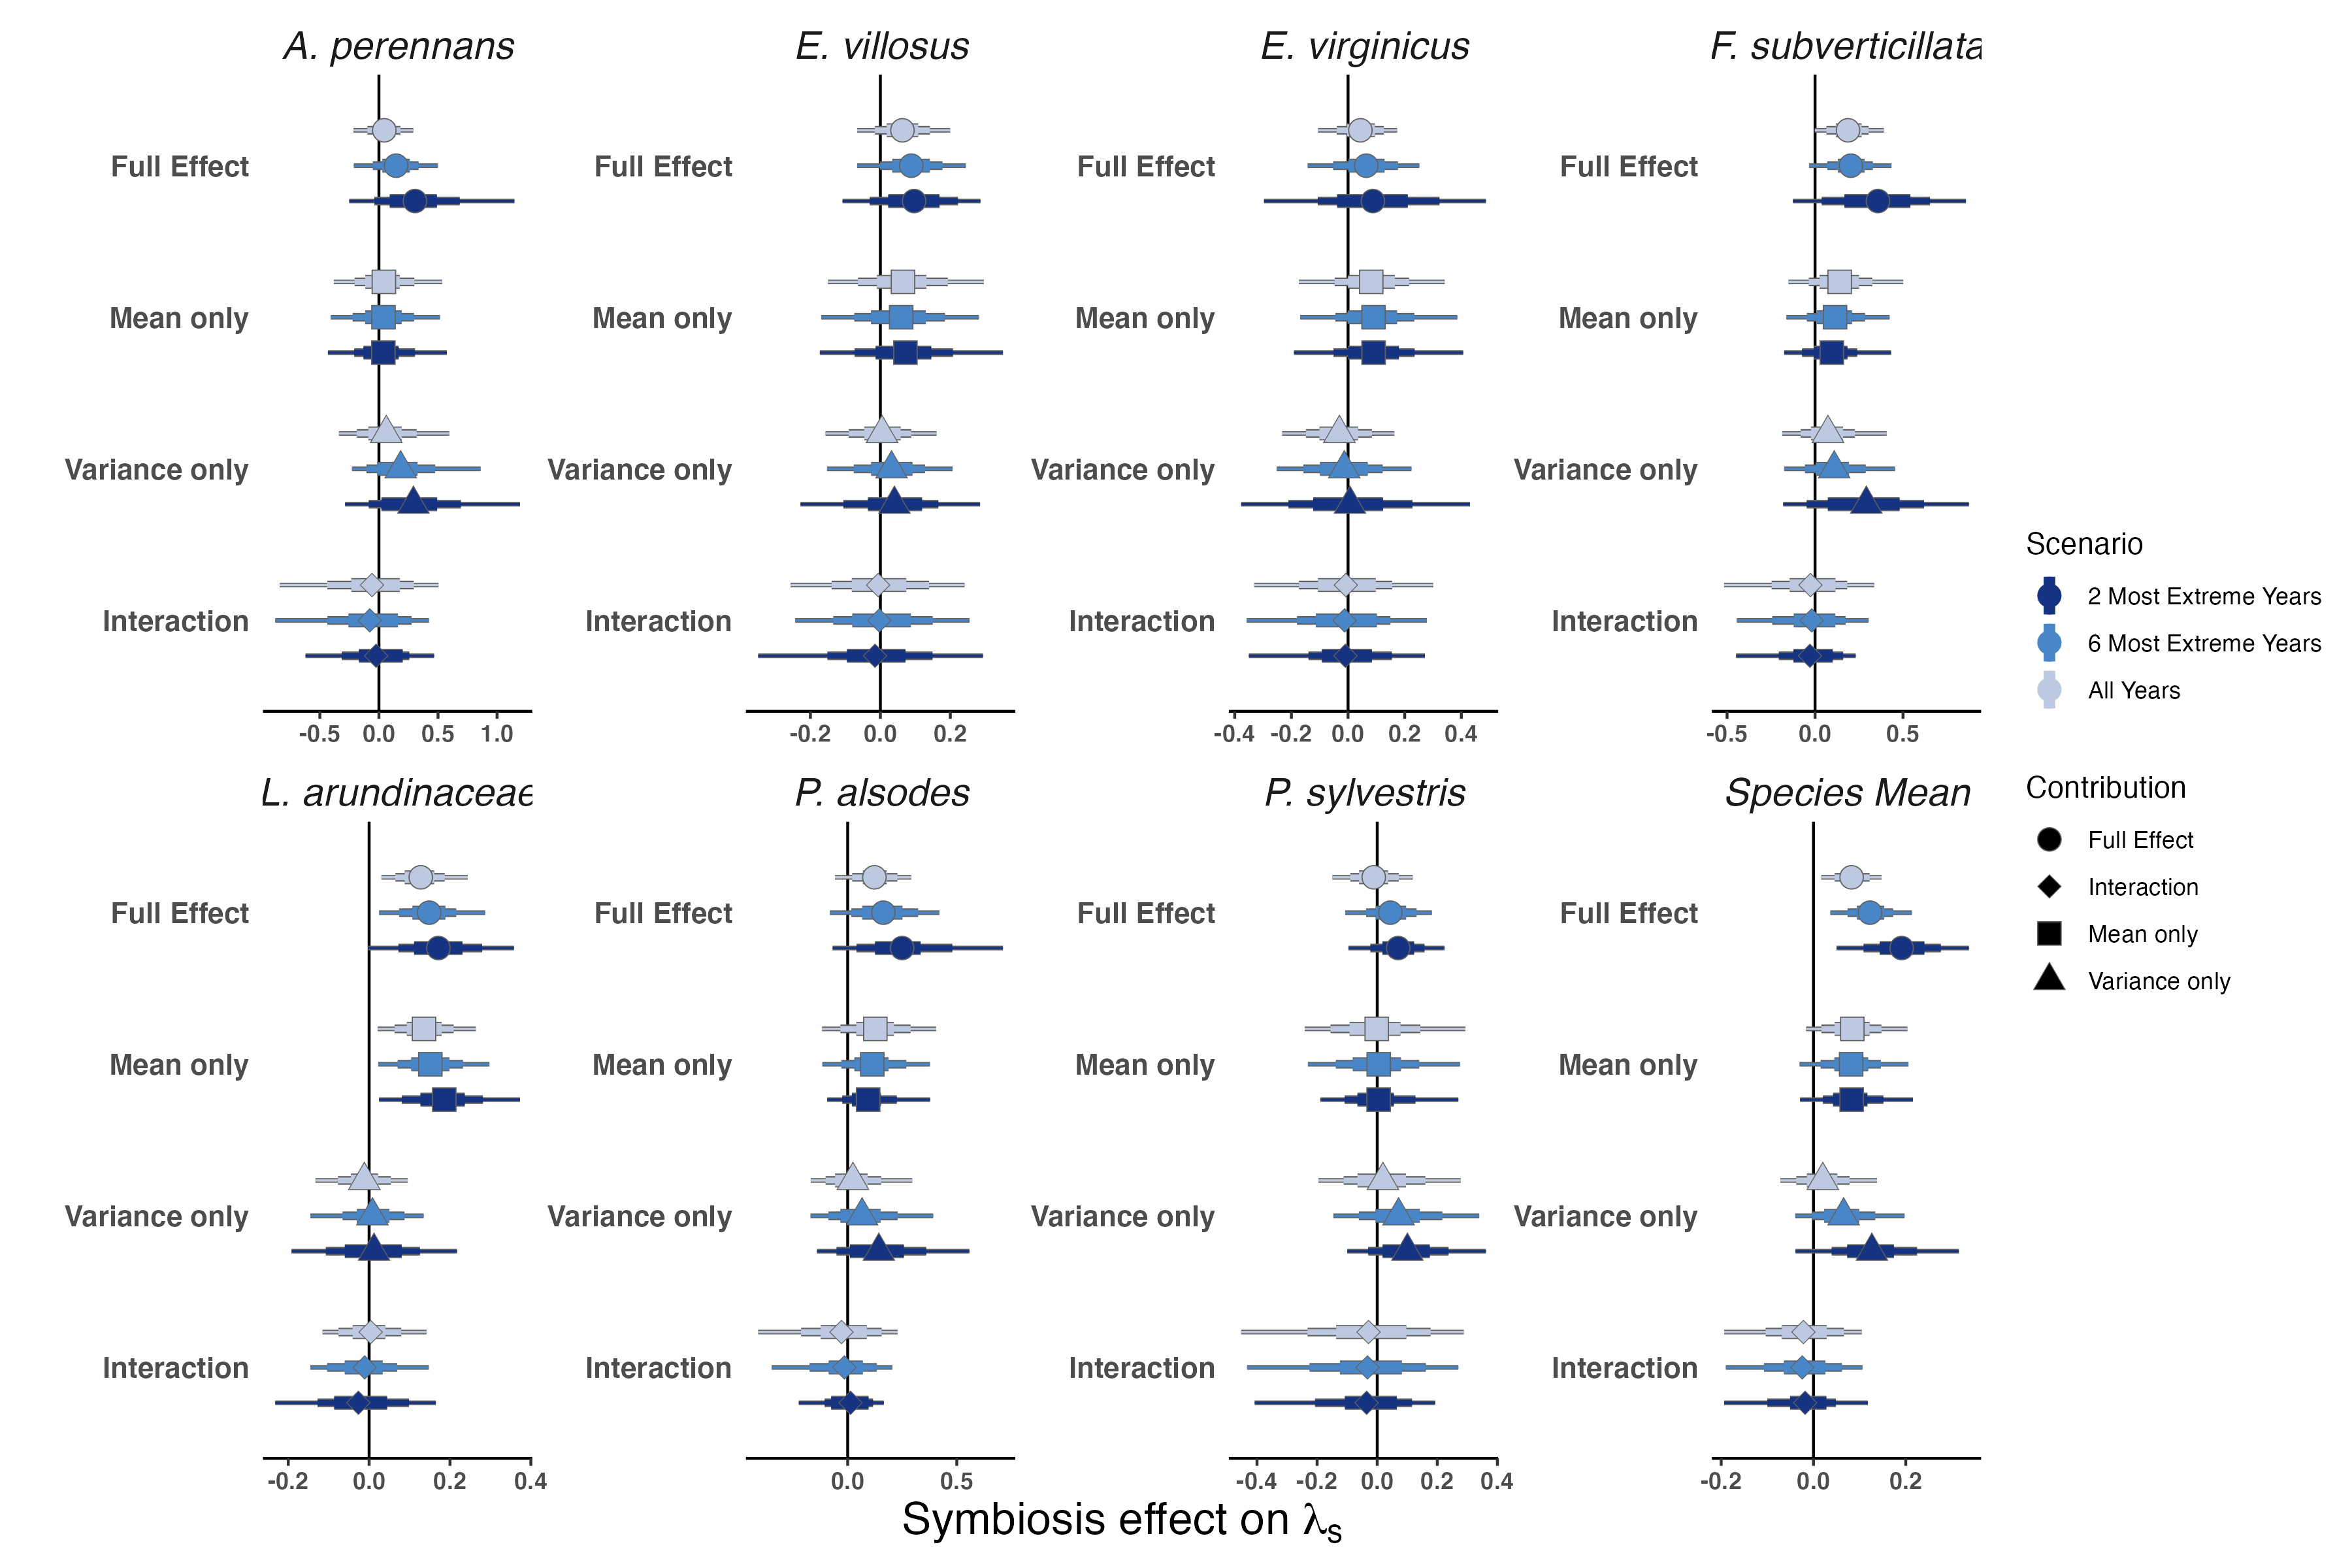
\includegraphics[width=\linewidth]{contributions_obs_plot.png}
\end{figure}
\noindent {\bf Fig. S21.} \textbf{Endophyte contributions to stochastic growth rates under observed and elevated variance across species.} The total effect of endophytes (circle) comes from mean benefits (square) and variance buffering (triangle) as well as the interaction between mean and variance effects (diamond). Shapes indicate the posterior mean of each contribution, along with bars for the 50, 75 and 95 \% credible intervals.  Under scenarios of increasing variance, represented by increasing color intensity, effects of variance buffering increase leading to a more mutualistic symbiosis.
\newpage

\begin{figure}
	\centering
	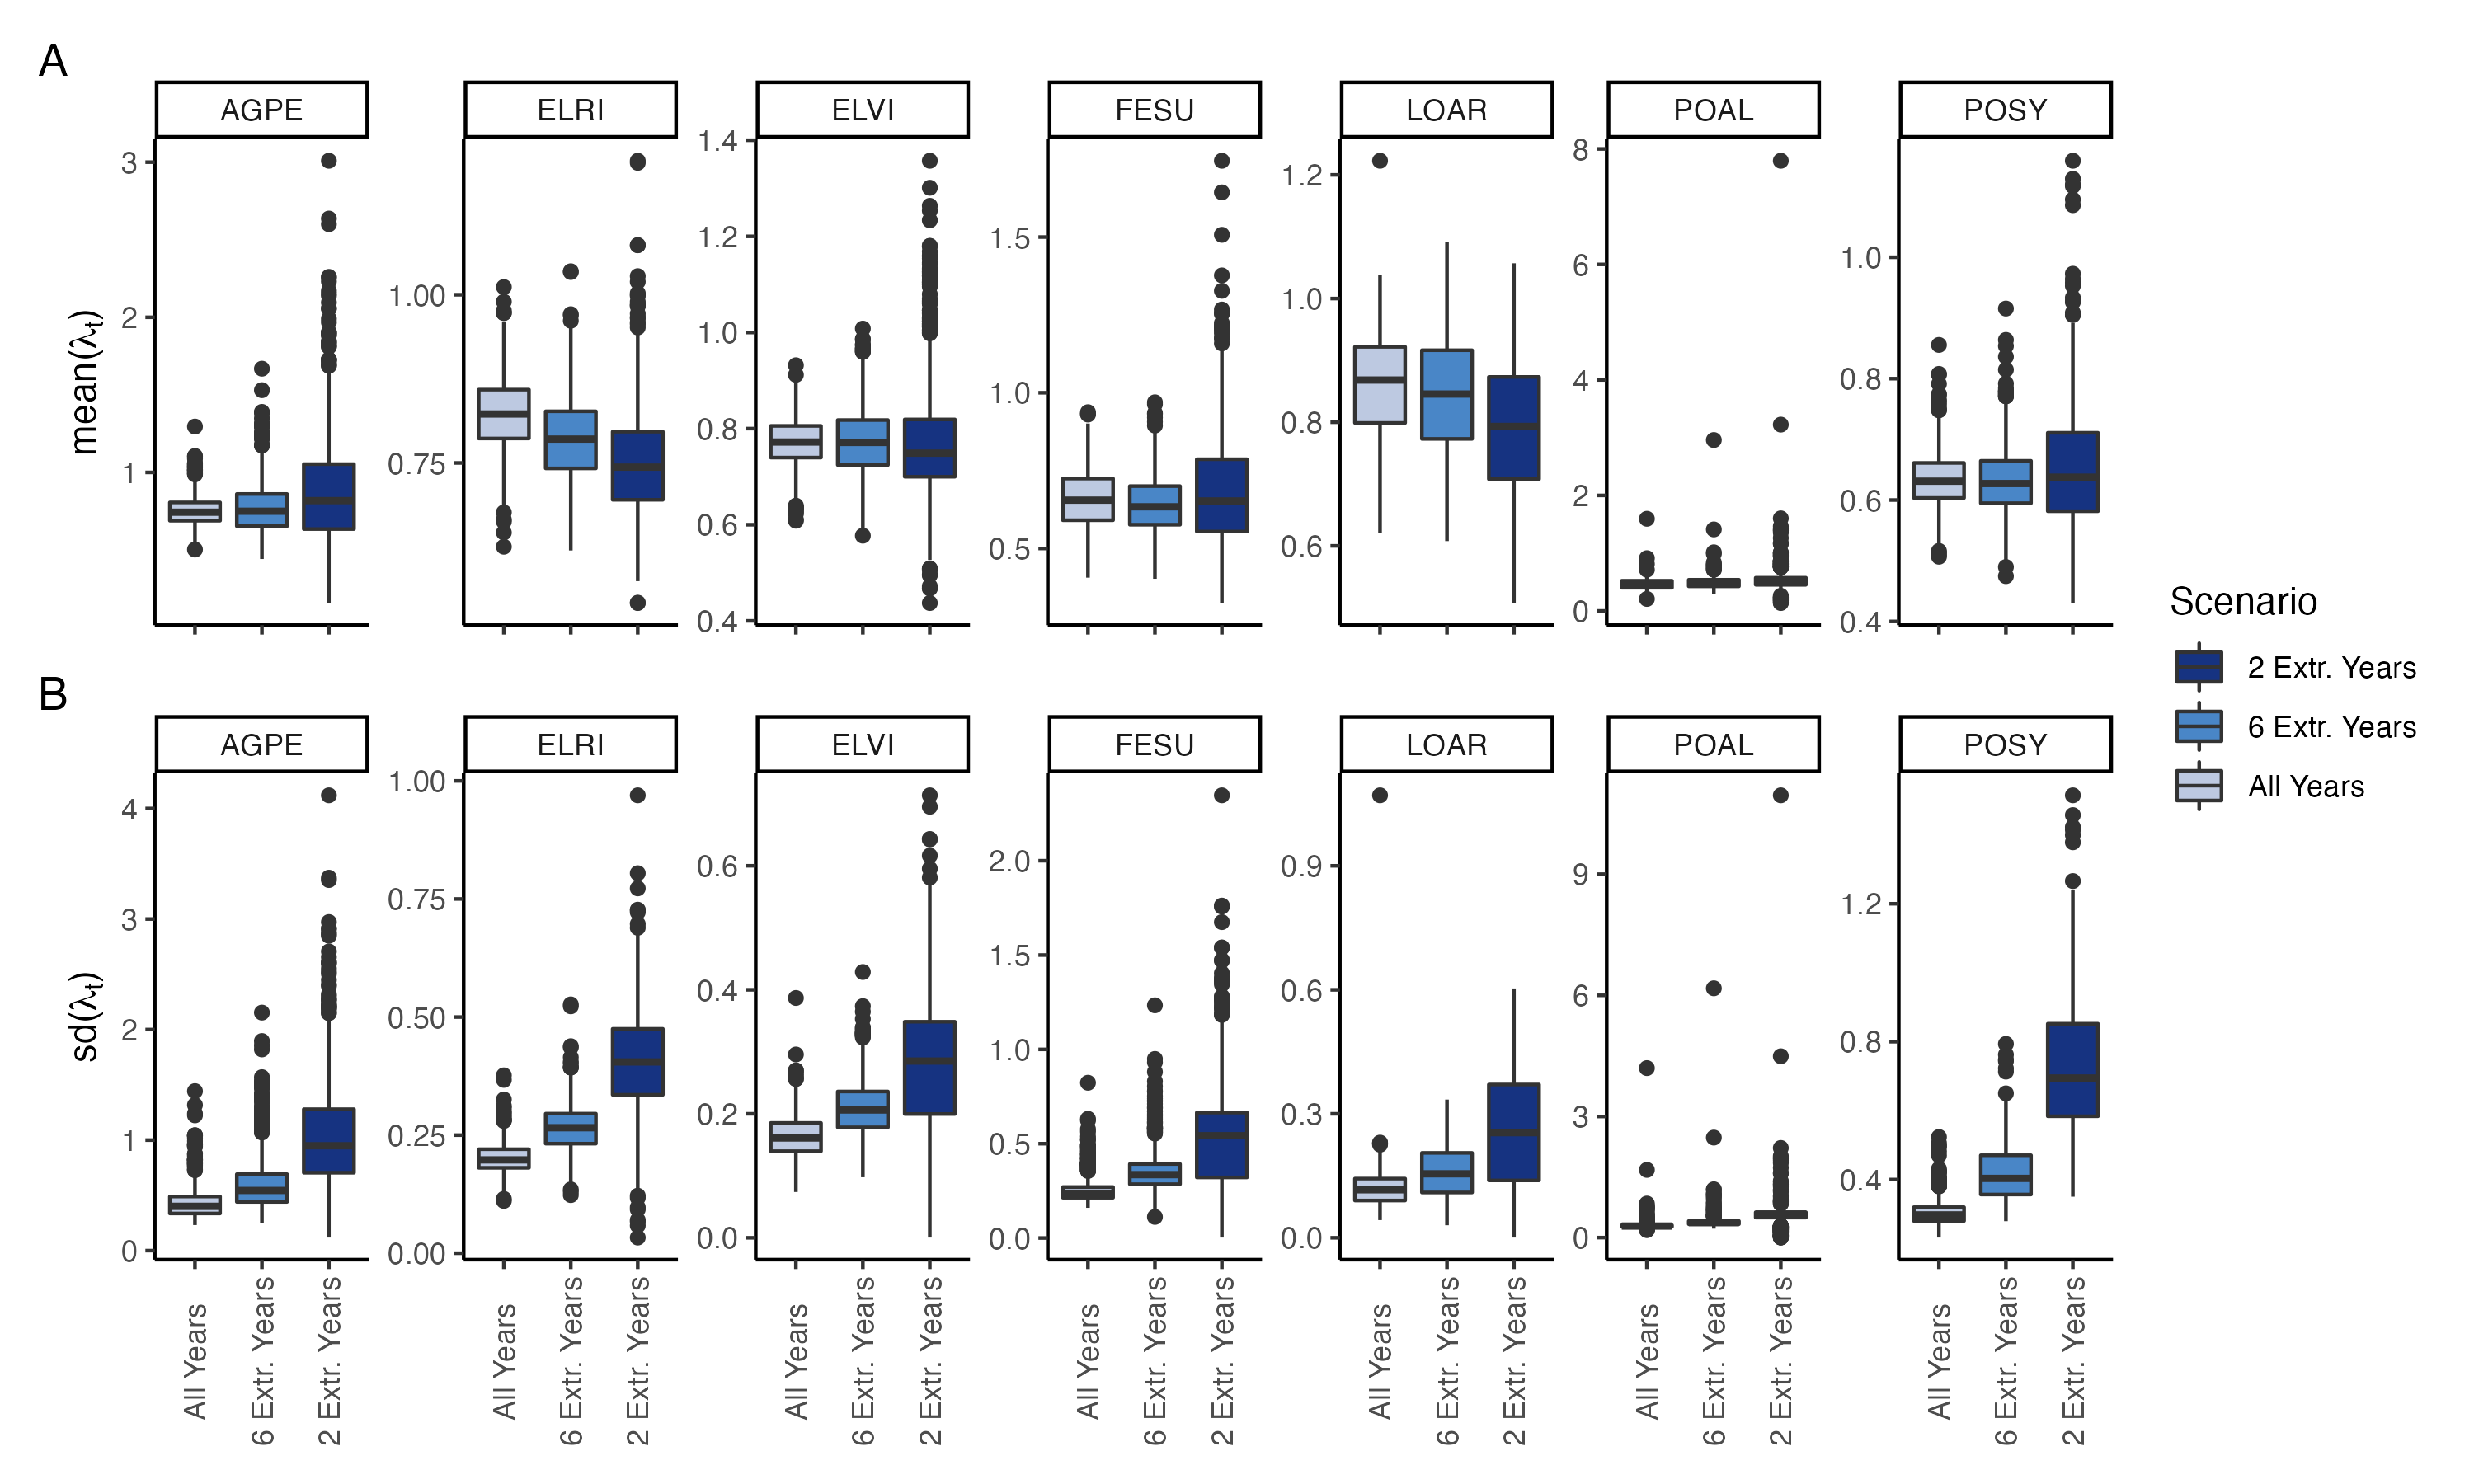
\includegraphics[width=\linewidth]{sim_boxplots.png}
\end{figure}
\noindent {\bf Fig. S22.} \textbf{(A) Mean and (B) standard deviation of annual growth rate values during simulation scenarios.} Each scenario selects from observed transition matrixes, increasing the variance by selecting either all observed years, or a set (6 or 2 years) that have the highest and lowest growth rates for symbiont-free populations.
\newpage


\begin{figure}
	\centering
	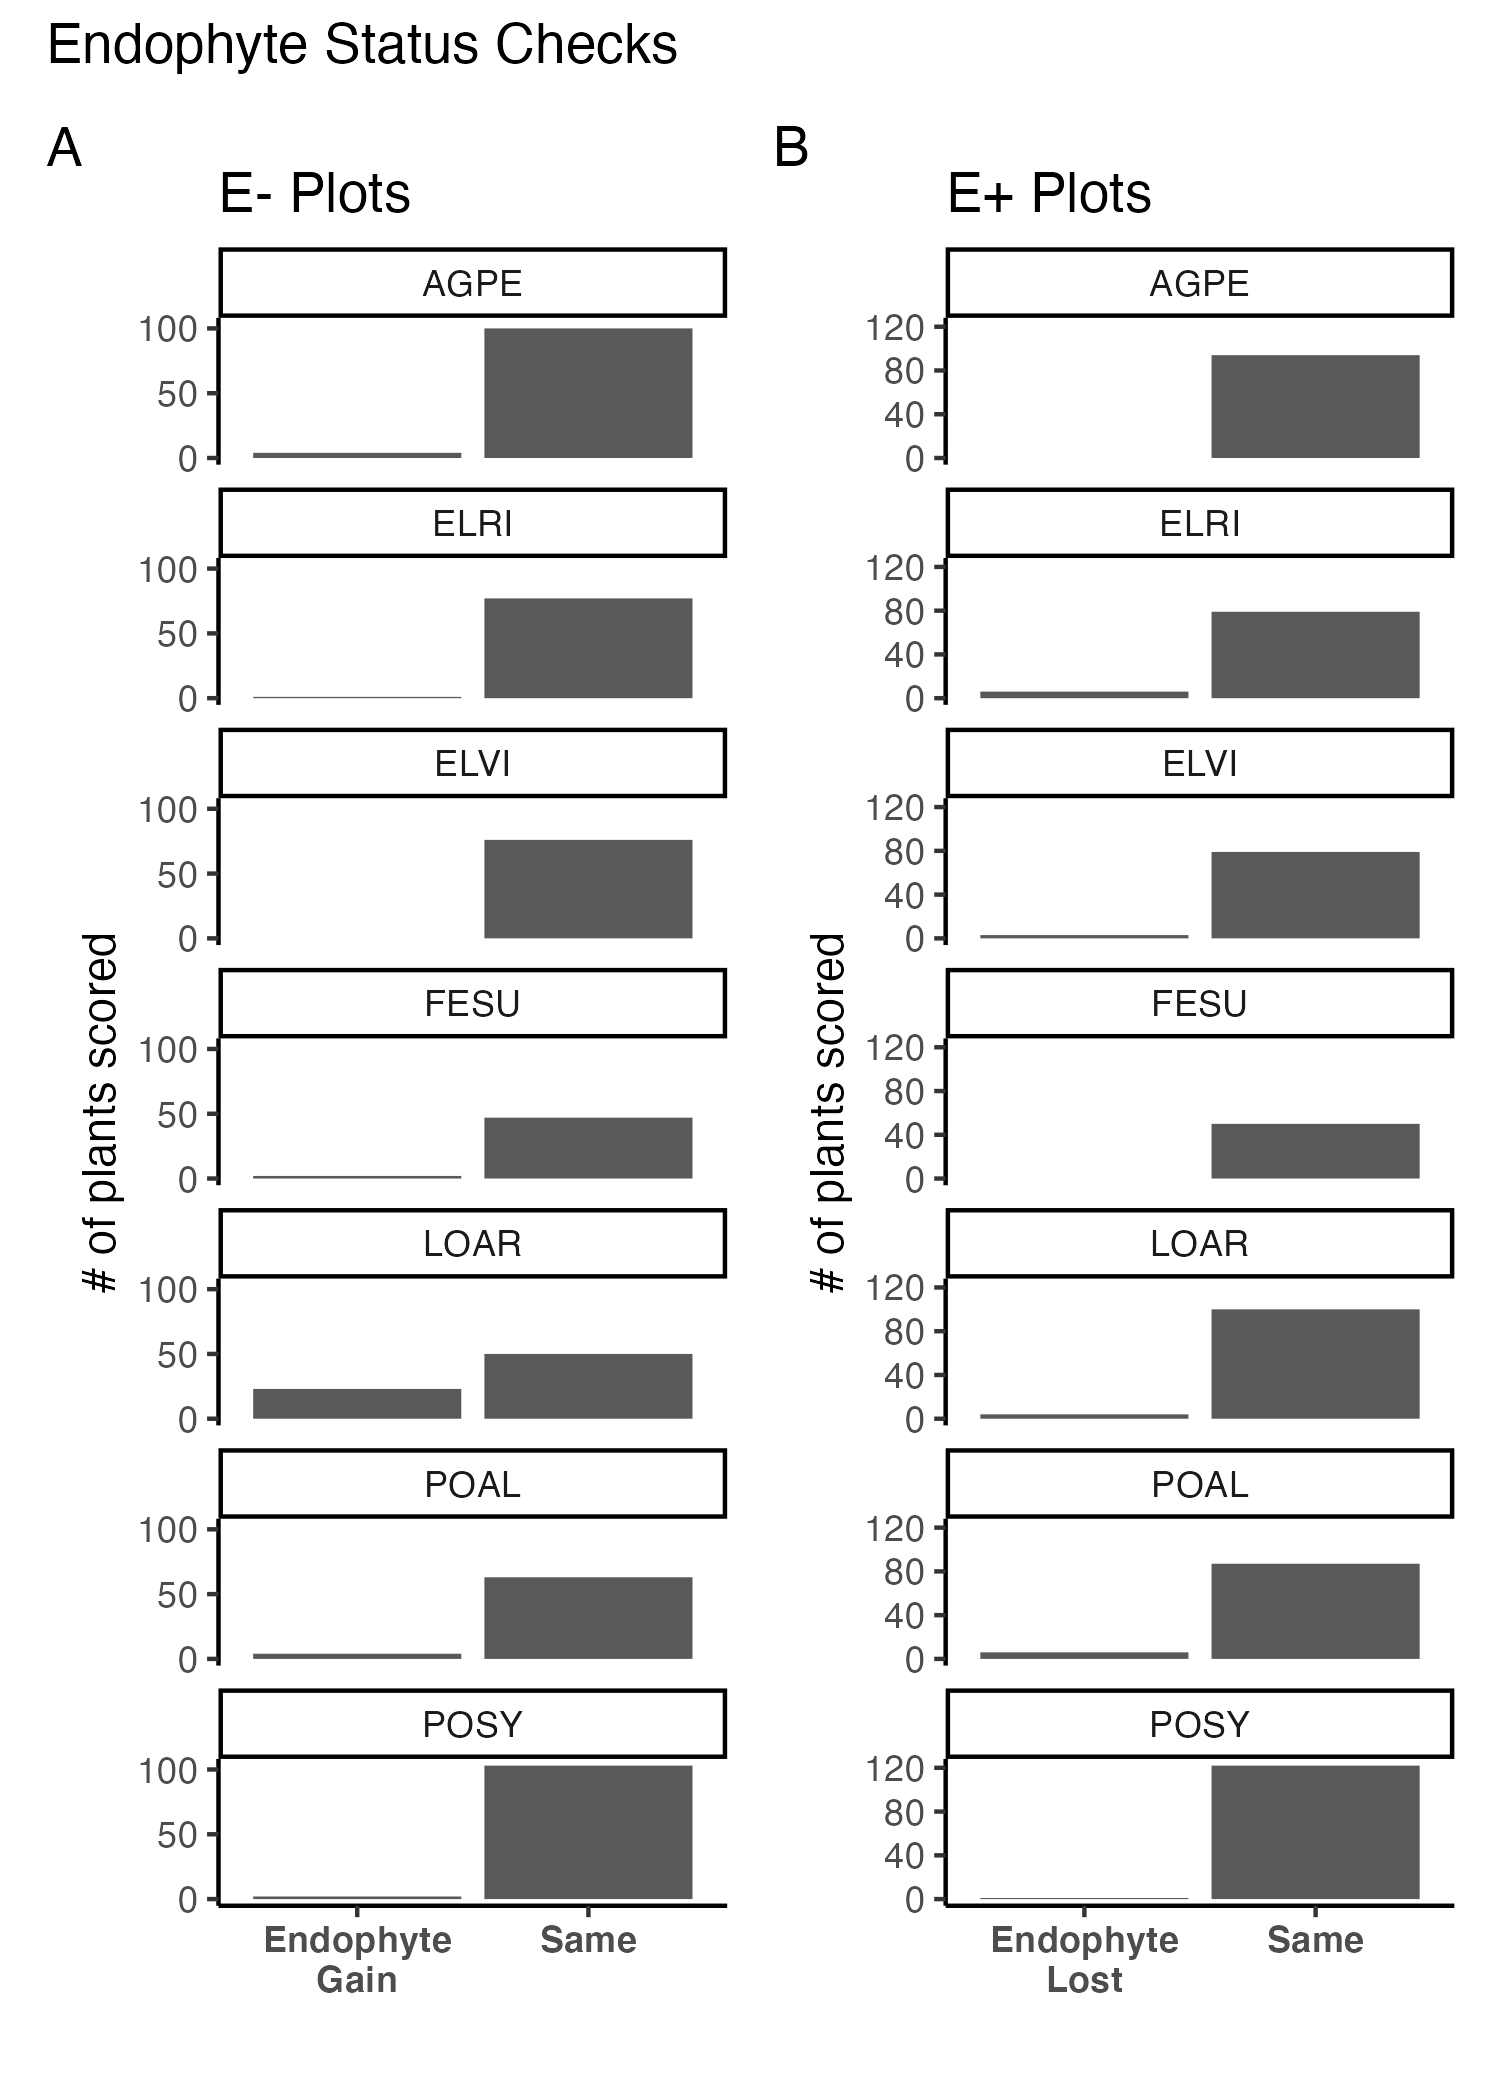
\includegraphics[width=.6\linewidth]{endo_check_plot.png}
\end{figure}
\noindent {\bf Fig. S23.} \textbf{Faithfulness of experimental plots to assigned endophyte status.} Counts of plants scored with leaf peels or seed squashes to check the faithfulness of recruits to the assigned plot-level endophyte status. (A) Endophytic plants may be gained in initially S- plots, or (B) lost in initially S+ plots.
\newpage

\begin{figure}
	\centering
	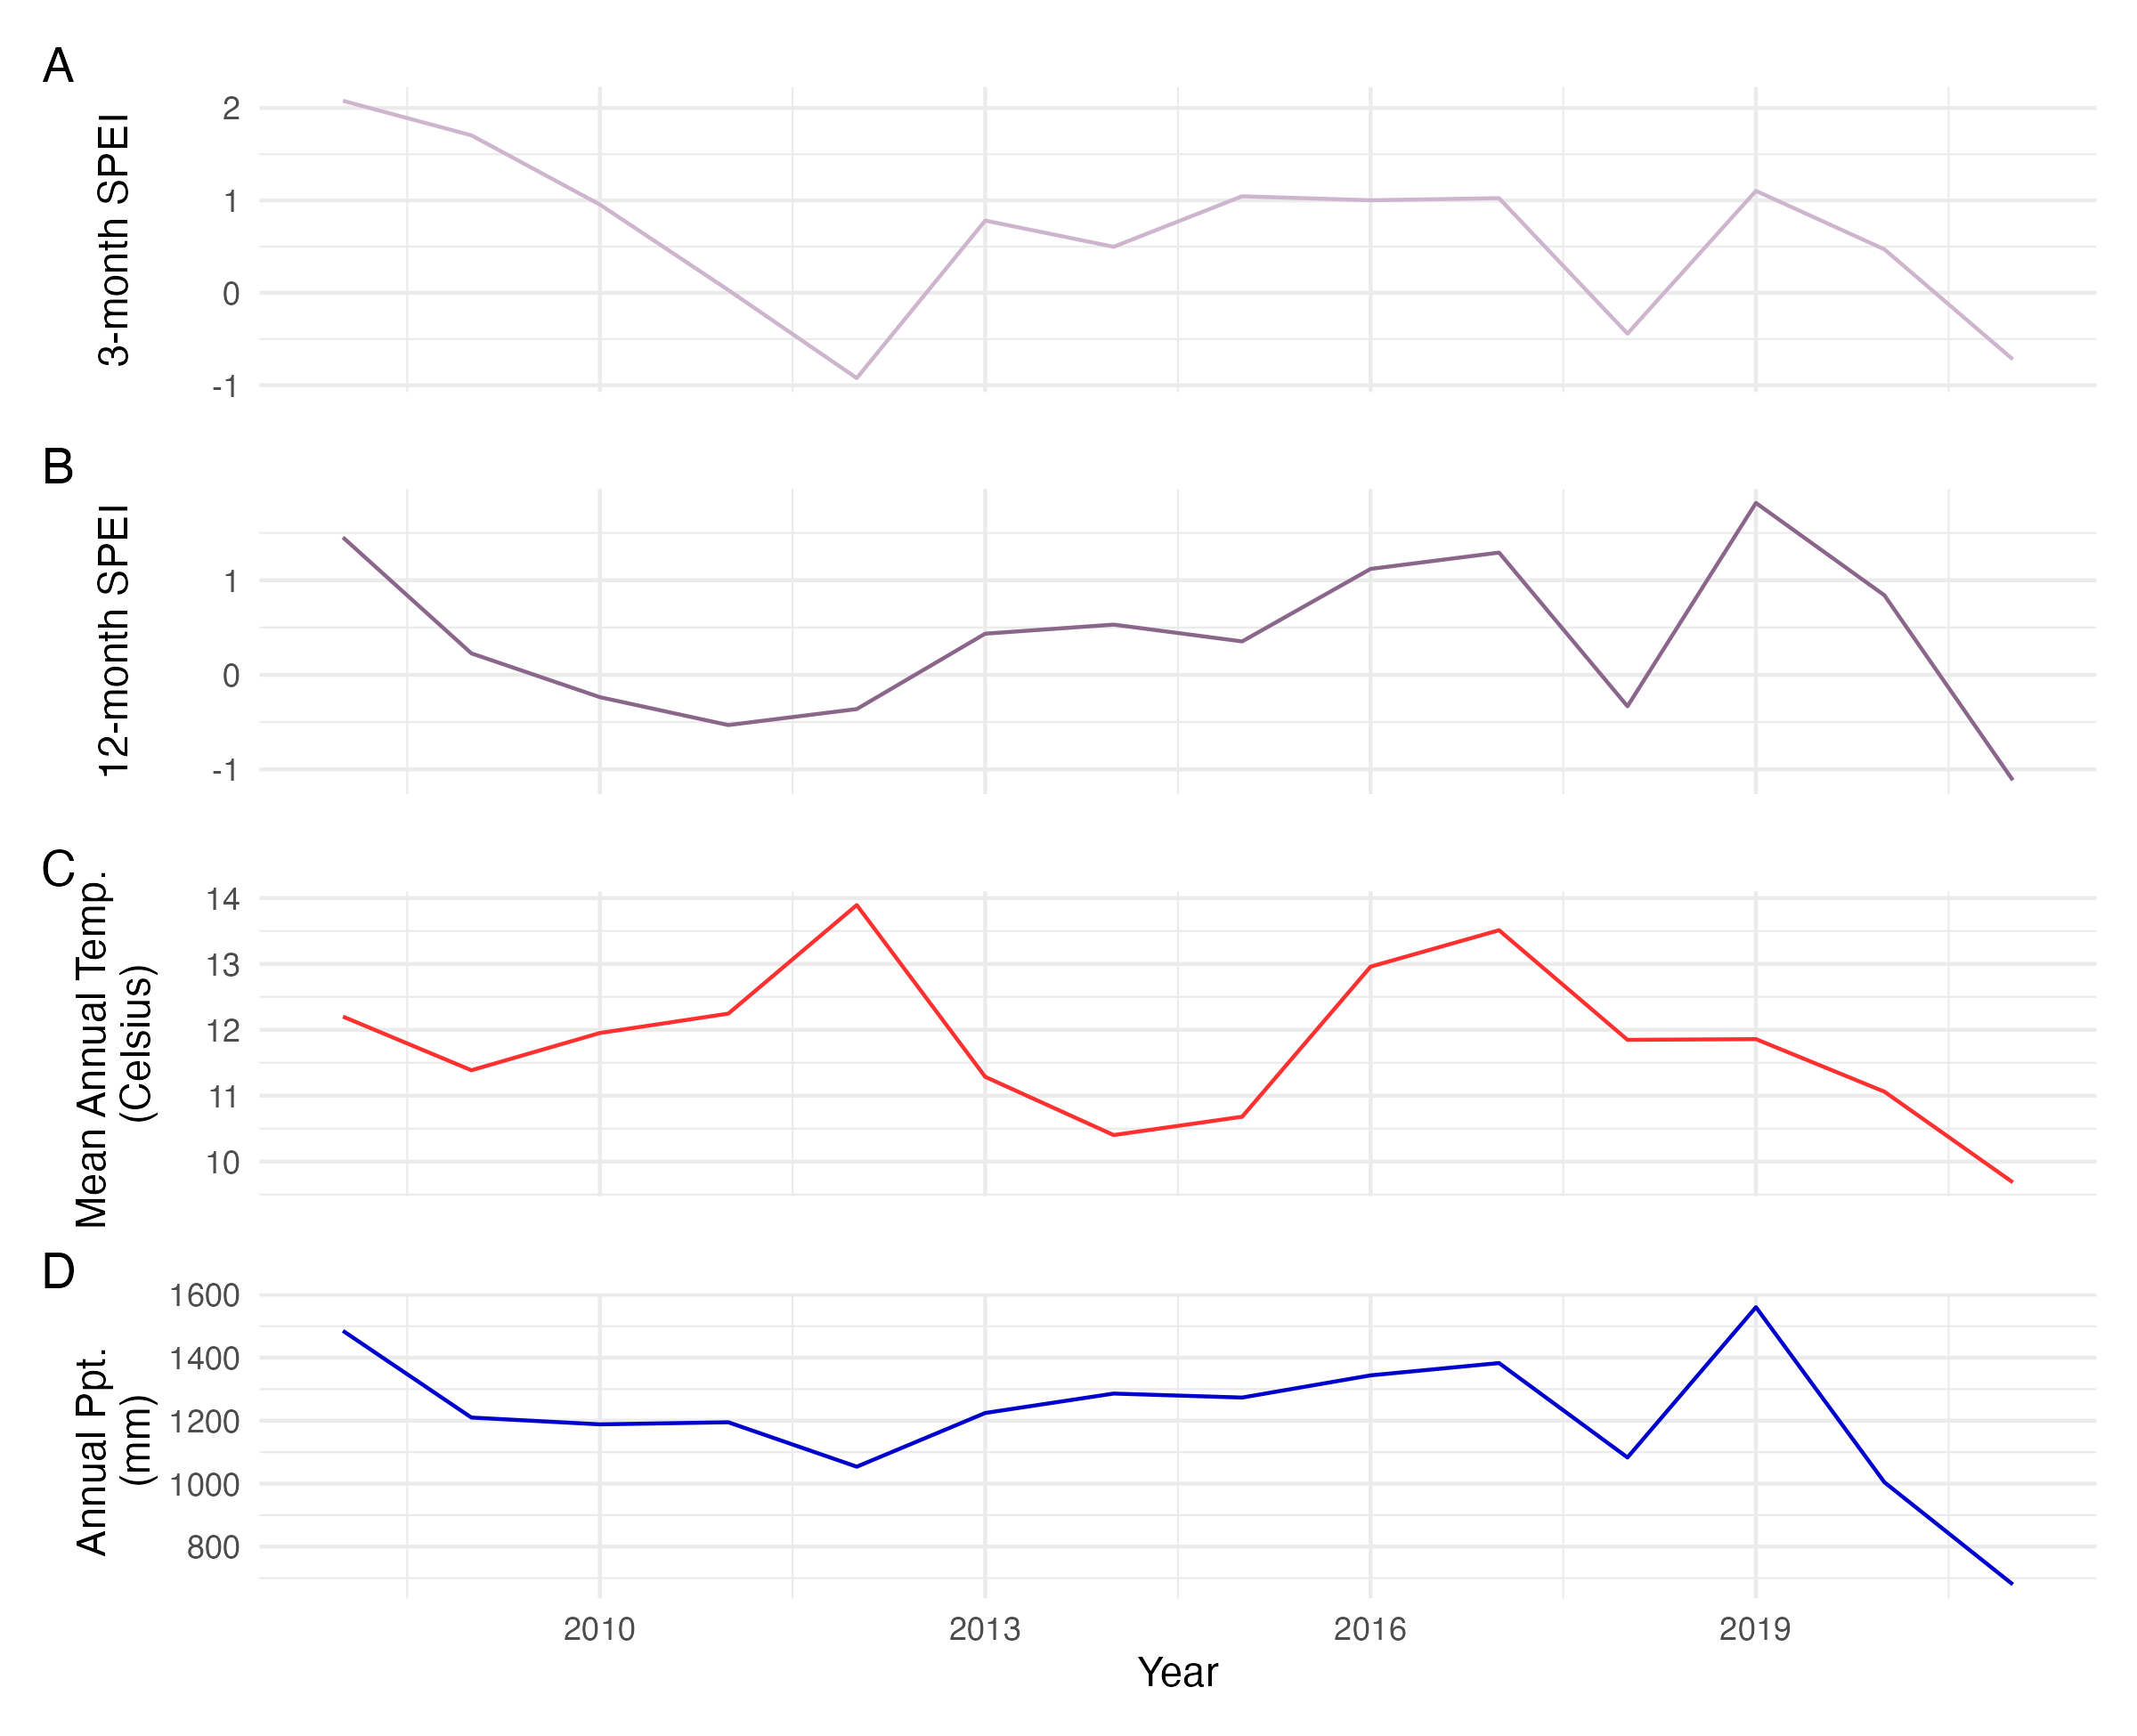
\includegraphics[width=\linewidth]{climate_plot.png}
\end{figure}
\noindent {\bf Fig. S24.} \textbf{Weather station time-series for Bloomington, IN.} The Seasonal Precipitation-Evapotranspiration Index (SPEI) calculated for the (A) three month growing season and (B) annually from daily weather station observations of (C) average temperatures and (D) cumulative precipitation. Climatic data shown are determined by the census year centered on the month of July. % when \emph{E. villosus} and \emph{E. virginicus}.
\newpage

\begin{figure}
	\centering
	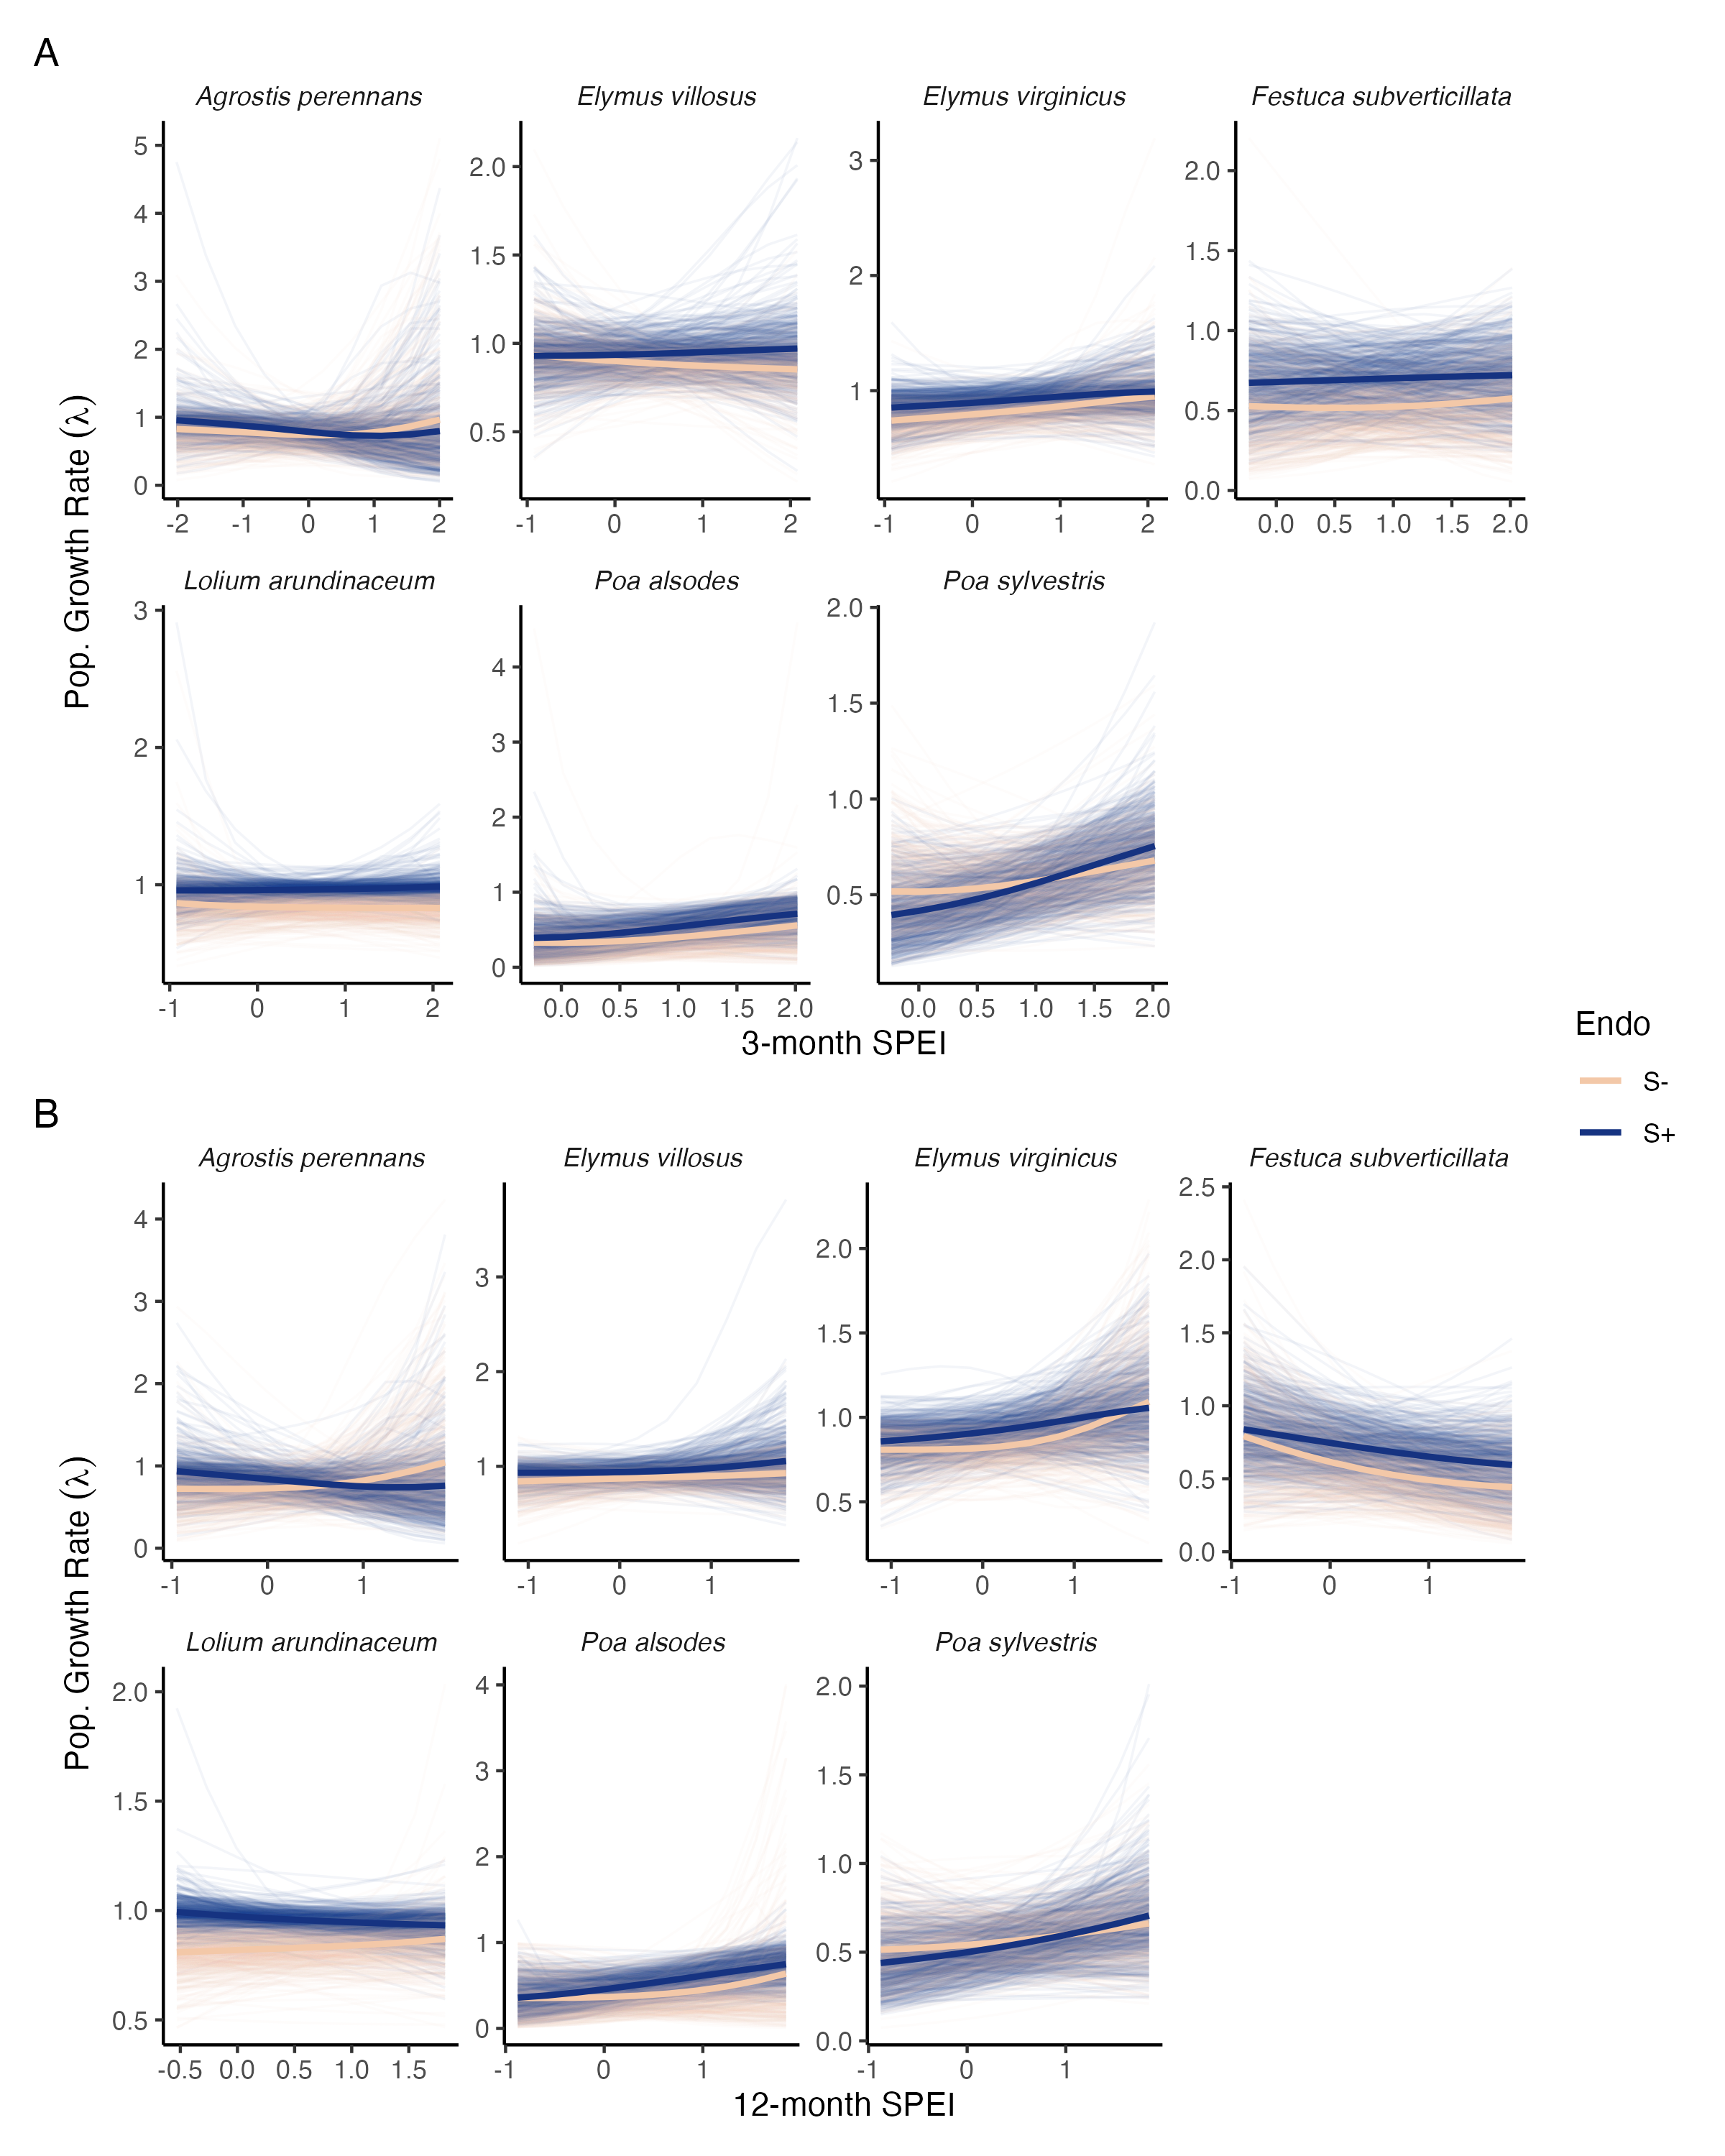
\includegraphics[width=.7\linewidth]{spei_combo_lambda_plot.png}
\end{figure}
\noindent {\bf Fig. S25.} \textbf{Predicted population growth rates across drought indices.} Symbiotic (S+; blue) and symbiont-free (S-; tan) populations respond differently to climate as measured by the (A) 3-month SPEI and (B) 12-month SPEI. Thick lines represent the predicted mean growth rate and thin lines show 500 posterior draws.
\newpage


\begin{figure}
	\centering
	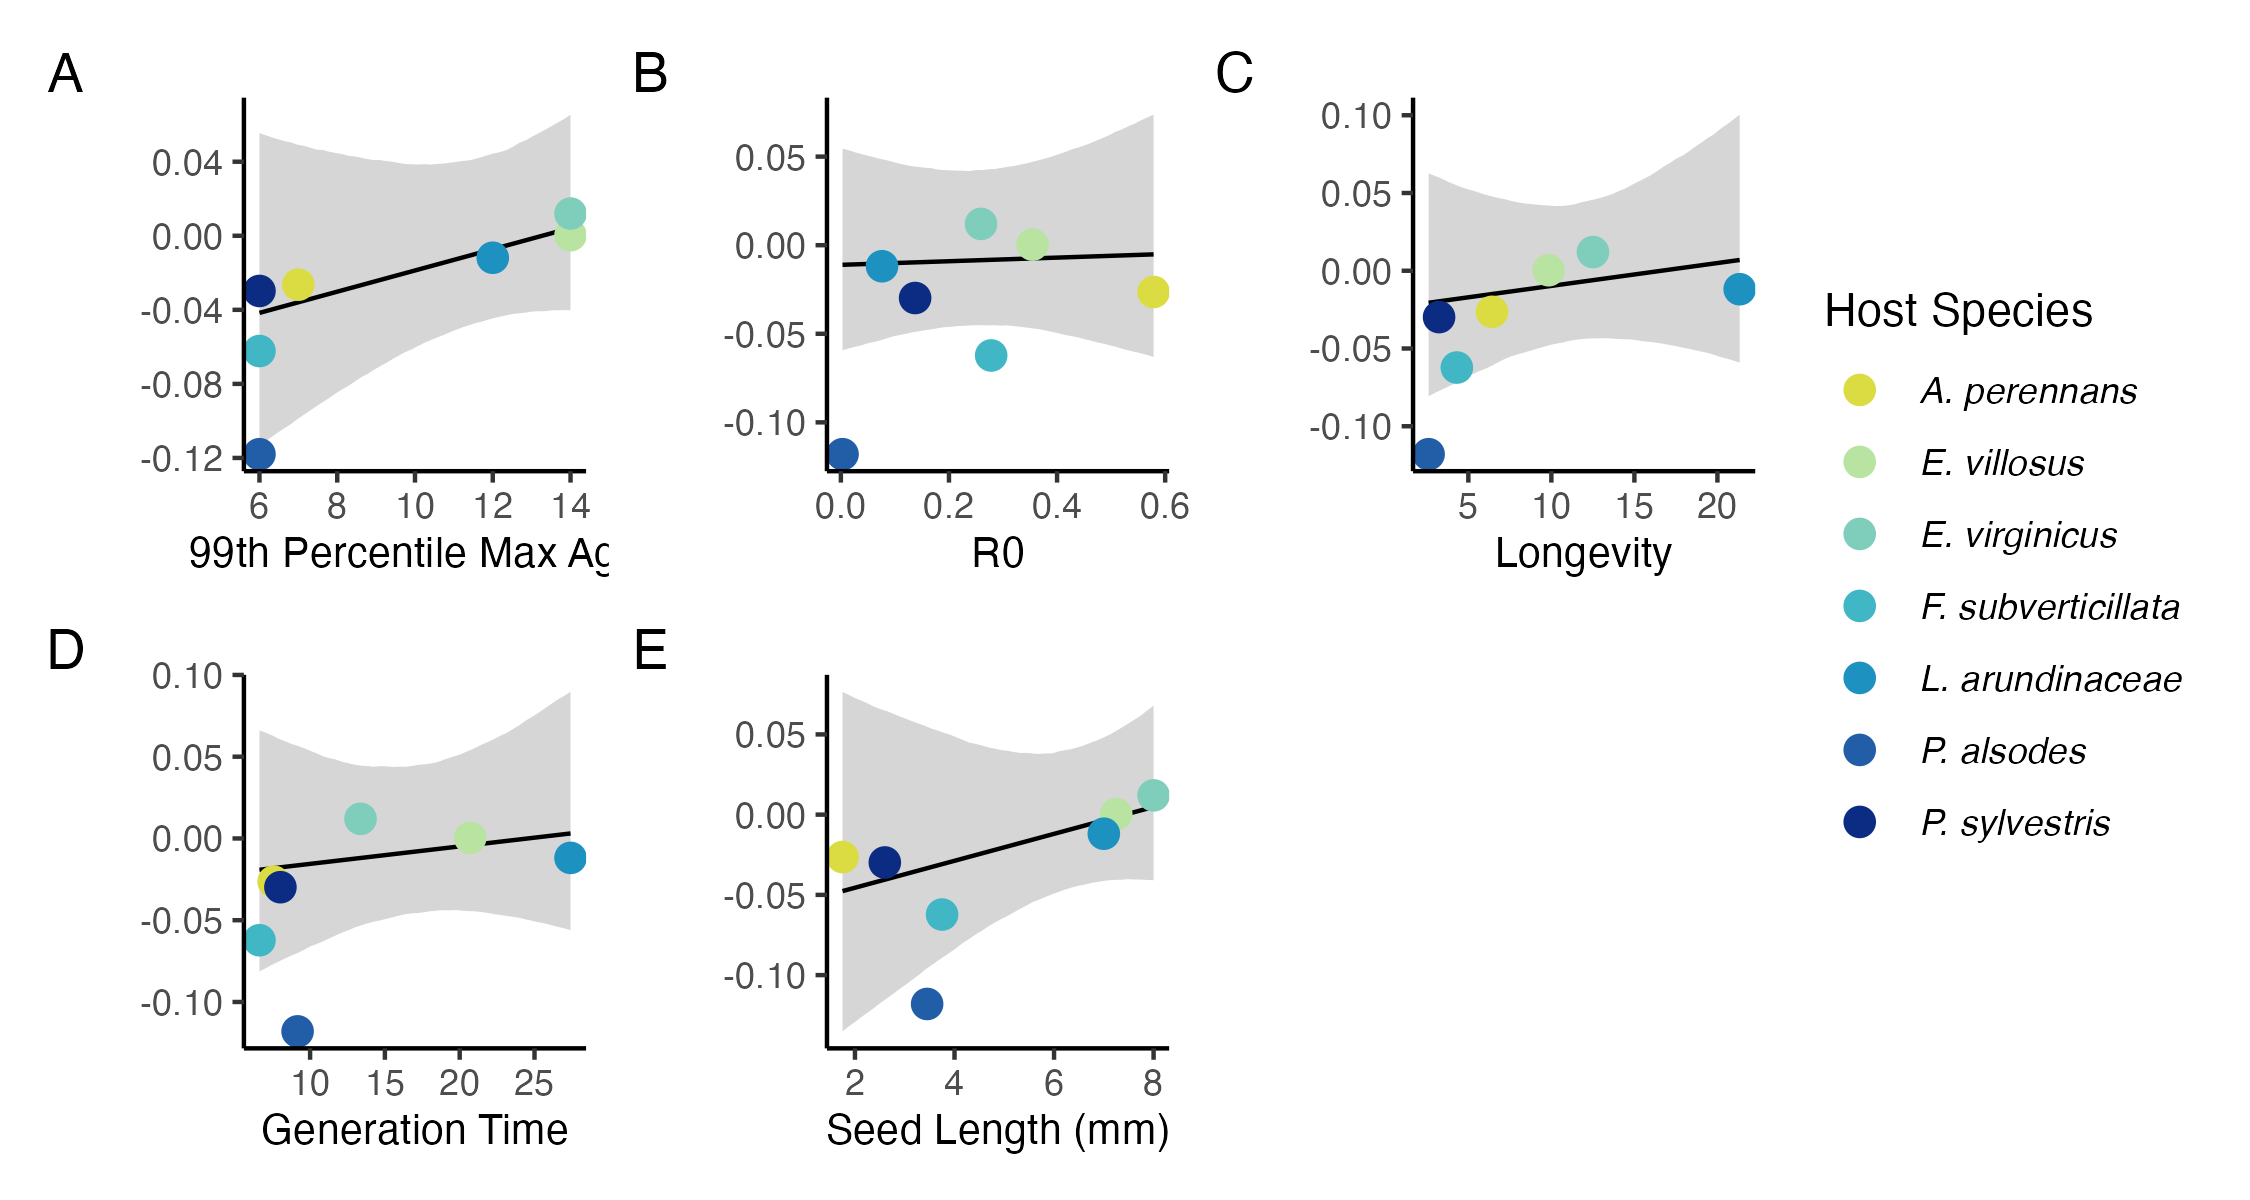
\includegraphics[width=\linewidth]{lh_epichloe_plot.png}
\end{figure}
\noindent {\bf Fig. S26.} \textbf{Relationship between variance buffering and life history traits describing the fast-slow life history continuum accounting for phylogenetic covariance between \emph{Epichlo\"{e}} symbionts.} Results are similar to regressions accounting for host plant phylogeny (Fig. 4), however symbionts are all within a single genus. Each panel shows the fitted mean relationship (line) along with with the 95\% credible interval.
\newpage


\begin{figure}
	\centering
	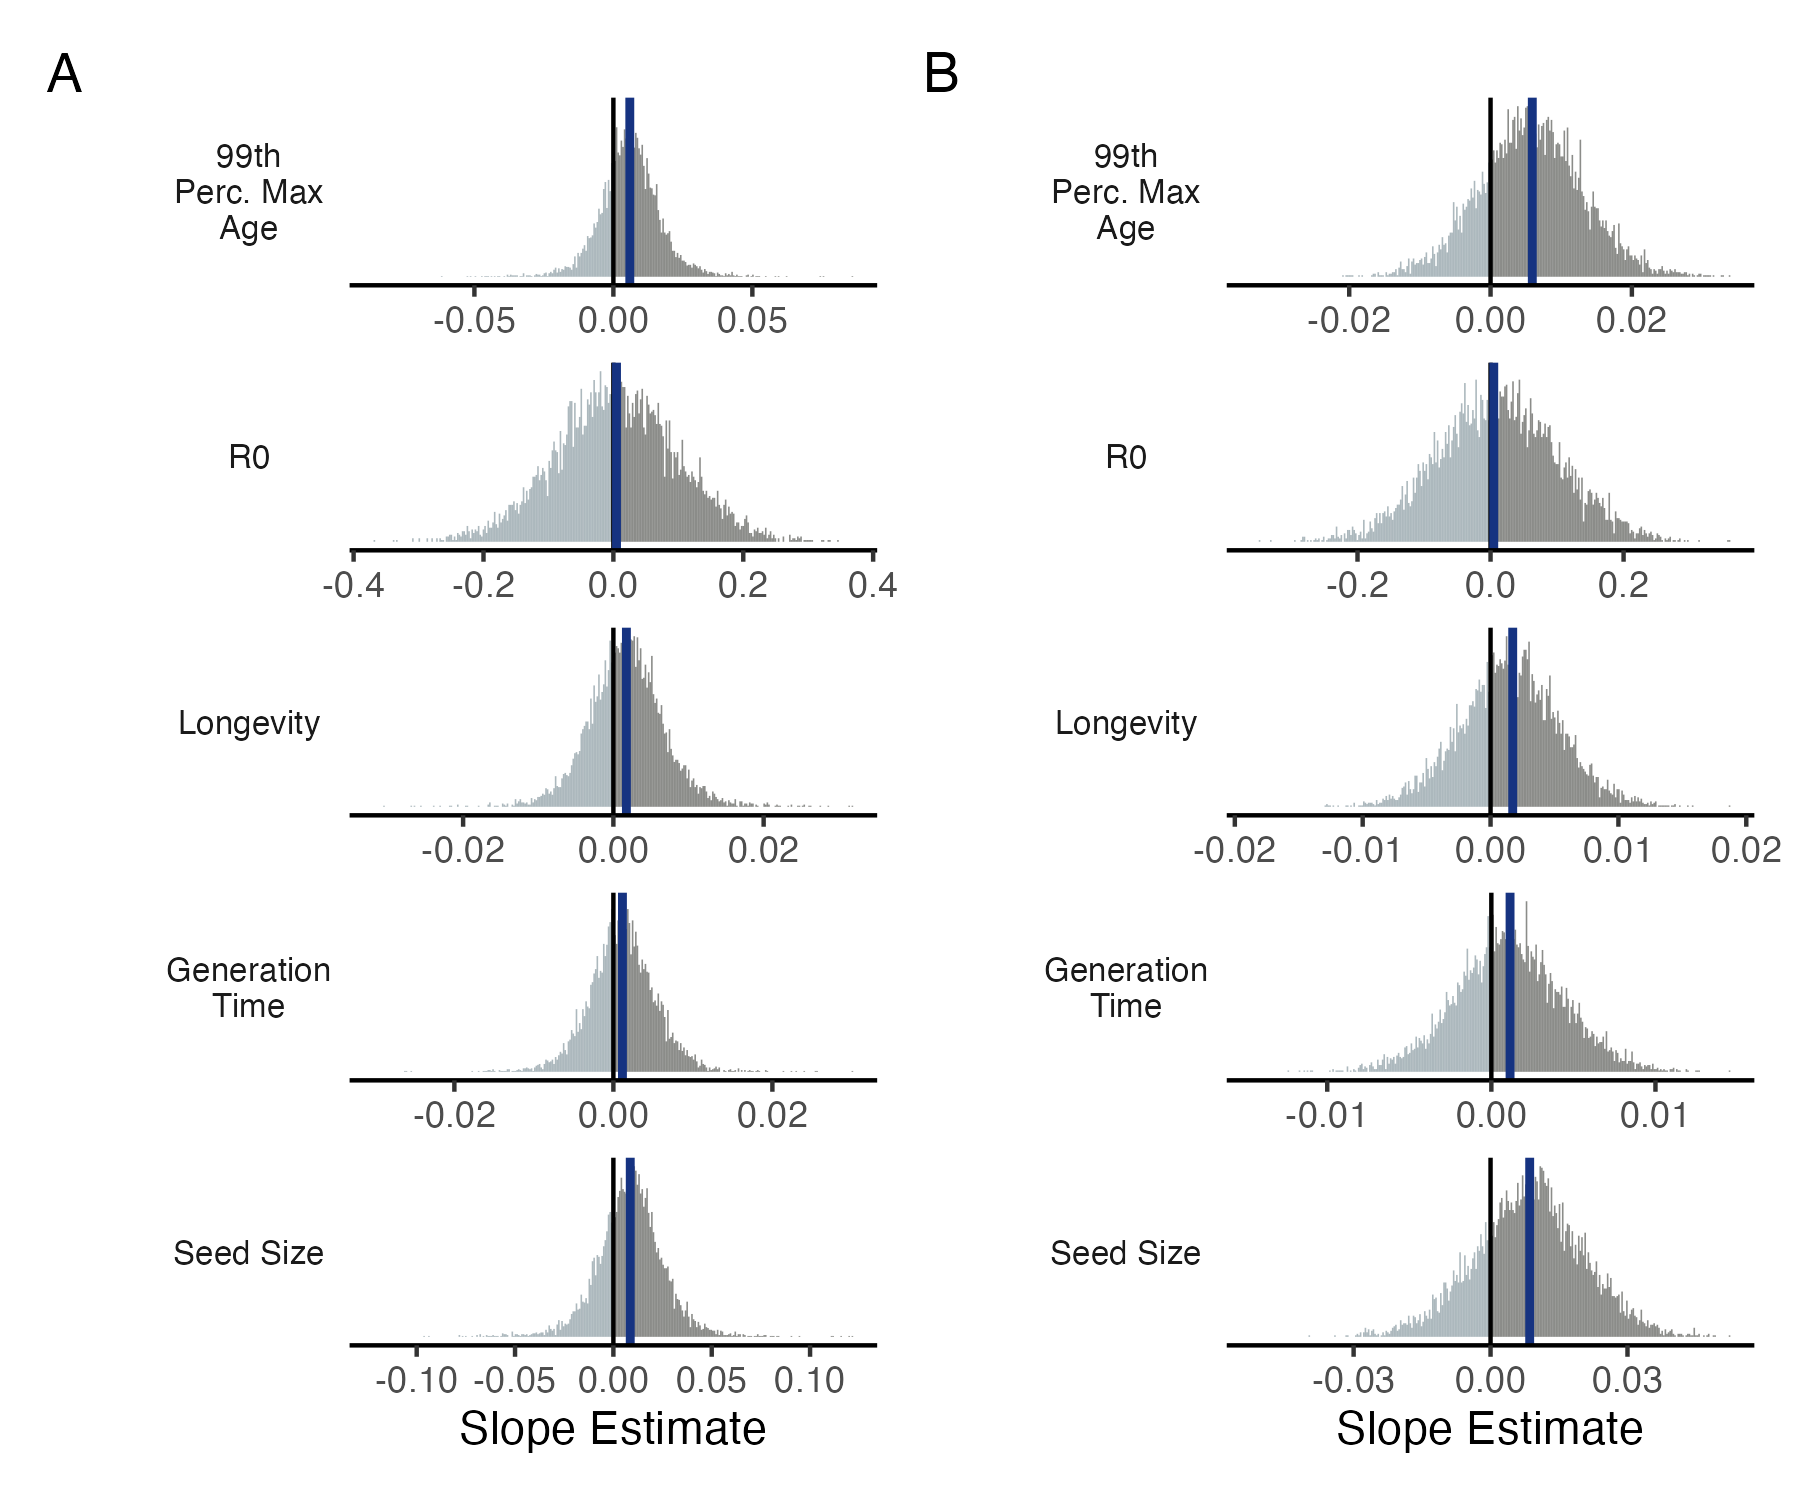
\includegraphics[width=.8\linewidth]{lh_slopes_plot.png}
\end{figure}
\noindent {\bf Fig. S27.} \textbf{Posterior estimates of life history trait effects on variance buffering.} Grey histograms show the posterior distribution of the slope parameter from models incorporating (A) host plant phylogenetic covariance and (B) symbiont phylogenetic covariance for each life history trait with blue bars showing the posterior mean.
\newpage




\noindent {\bf Table S1.} Summary of host-endophyte proprogation and transplant methods\\
\begin{table}[ht]
	\begin{adjustbox}{width=1\textwidth}
\begin{tabular}{|l|l|l|l|}
\hline
	\bf{Host Species} & \bf{Symbiont Species} & \bf{Heat treatment duration (Temp.)}& \bf{Transplant date }\\
	        \hline
	\emph{Agrostis perennans} & \emph{E. amarillans}&12 min. hot water bath (60 $^{\circ}$C)&April 2008 (10 plots)\\
	\emph{Elymus villosus} &\emph{E. elymi}&6 days drying oven (60 $^{\circ}$C)&April 2008 (10 plots)\\
	\emph{Elymus virginicus} &\emph{E. elymi or EviTG-1}&6 days drying oven (60 $^{\circ}$C)&April 2008 (10 plots)\\
	 \emph{Festuca subverticillata} &\emph{E. starrii}&6 days drying oven (60 $^{\circ}$C)&April 2008 (10 plots)\\
	 \emph{Lolium arundinaceum} &\emph{E. coenophiala}&6 days drying oven (60 $^{\circ}$C)& Sept. 2007 (10 plots)\\
	 \emph{Poa alsodes} &\emph{E. alsodes}& 7 days drying oven (60 $^{\circ}$C)&Sept. 2007 (8 plots)/April 2008 (10 plots)\\
	 \emph{Poa sylvestris}&\emph{E. PsyTG-1}&7 days drying oven (60 $^{\circ}$C)& Sept. 2007 (8 plots)/April 2008 (10 plots)\\
	 \hline
\end{tabular}
\end{adjustbox}
\end{table}


%\tom{(6d in a drying oven at 60$^{\circ}$ C for \emph{E. villosus}, \emph{E. virginicus}, \emph{F. subverticillata},  and \emph{L. arundinaceum}; 7d in a drying oven at 60$^{\circ}$ C for \emph{P. alsodes}, and \emph{P. sylvestris}; and 12 min. in a hot water bath at 60$^{\circ}$ C for \emph{A. perennans})}{need to double check methods for temp, duration, etc.}



\noindent {\bf Table S2.} Summary of focal life history traits \\
\begin{table}[ht]
\begin{adjustbox}{width=1\textwidth}{
\begin{tabular}{|p{4cm}| p{2cm} |p{2cm}|p{2cm}| p{1cm}|p{2cm}|p{2cm}|p{2.5cm}| p{2cm}|}
	\hline
	\bf{Host Species} & \bf{Observed max age}& \bf{99th perc. max age}&\bf{Generation time} & $\mathbf{R}_0$ &\bf{Longevity}&\bf{Seed Length (mm.)}&\bf{Imperfect transmission rate} & \bf{Stromata Observed}\\
	\hline
	\emph{Agrostis perennans} &11&7&7.6&0.58&6.4&1.75&69.8&No\\
	\emph{Elymus villosus}, &14&14&20.7&0.35&9.8&7.25&100&Yes\\
	\emph{Elymus virginicus} &14&14&13.4&0.25&12.5&8&100&Yes\\
	\emph{Festuca subverticillata} &9&6&6.6&0.28&4.3&3.75&42.7&No\\
	\emph{Lolium arundinaceum} &12*&12*&27.4&0.08&21.3&7&100&No\\
	\emph{Poa alsodes} &8&6&9.2&0.003&2.6&3.45&99.9&No\\
	\emph{Poa sylvestris}&12&6&8.0&0.14&3.2&2.6&16.6&Yes\\
	 \hline
\end{tabular}}
\end{adjustbox}
\end{table}

* Censuses for \emph{L. arundinaceum} plots stopped after year 12 of the experiment.


\noindent {\bf Table S3.} Summary of host-endophyte drought sensitivities\\
\begin{table}[ht]
	\begin{adjustbox}{width=1\textwidth}{
			\begin{tabular}{|p{4cm}| p{2cm} |p{2cm}|p{2cm}|p{2cm}| p{2cm}|p{2cm}|p{2cm}|p{2cm}|}
				\hline
				\bf{Host Species} & \bf{Effect on CV($\lambda$)}& \bf{Effect on Mean($\lambda$)}&$\frac{\Delta\lambda_{E-}}{\Delta SPEI_{3}}$ & $\frac{\Delta\lambda_{S+}}{\Delta SPEI_{3}}$ &\bf{3 month S- to S+ ratio}&$\frac{\Delta\lambda_{E-}}{\Delta SPEI_{12}}$ &$\frac{\Delta\lambda_{S+}}{\Delta SPEI_{12}}$ &\bf{12 month S- to S+ ratio}\\
				\hline
				\emph{Agrostis perennans} &-0.02641&0.04412&0.0341&-0.0400&0.85&0.11410&-0.06255&1.82\\
				\emph{Elymus villosus}, &0.00033&0.05089&-0.0267&0.0137&1.95&0.02968&0.04216&0.70\\
				\emph{Elymus virginicus} &0.01201&0.05775&0.0697&0.0465&1.50&0.09677&0.06803&1.42\\
				\emph{Festuca subverticillata} &-0.06225&0.16393&0.0213&0.0212&1.01&-0.12873&-0.09010&1.43\\
				\emph{Lolium arundinaceum} &-0.01188&0.10215&-0.0119&0.0090&1.32&0.02644&-0.02596&1.02\\
				\emph{Poa alsodes} &-0.11798&0.12816&0.1017&0.1429&0.71&0.10457&0.14328&0.73\\
				\emph{Poa sylvestris}&-0.02981&-0.00852&0.0717&0.1600&0.44&0.05445&0.09820&0.55\\
				\hline
		\end{tabular}}
	\end{adjustbox}
\end{table}



\end{document}





















